% !TeX program = pdflatex
\documentclass[11pt,twoside]{book}

% ---------------------------------------------
% Kindle-friendly symmetric margins, 6x9
% ---------------------------------------------
\usepackage[
  paperwidth=6in,
  paperheight=9in,
  includehead,
  includefoot,
  heightrounded,
  top=0.8in,
  bottom=0.8in,
  inner=0.8in,
  outer=0.8in
]{geometry}

% ---------------------------------------------
% Typography
% ---------------------------------------------
\usepackage[T1]{fontenc}
\usepackage[utf8]{inputenc}
\usepackage{microtype}
\usepackage{lmodern}
\linespread{1.08}
\setlength{\parskip}{0.4em}
\setlength{\parindent}{1.2em}

% ---------------------------------------------
% Ancient Greek (polytonic) with pdfLaTeX
% ---------------------------------------------
\usepackage[greek,english]{babel}   % language switching (LGR for Greek)
\languageattribute{greek}{polutoniko}
\usepackage{alphabeta}              % type Greek in UTF-8 under pdfLaTeX

%--------------------------------------------------
% Title Page
%--------------------------------------------------
% ---------------------------------------------
% Headers/Footers
% ---------------------------------------------
\usepackage{fancyhdr}
\setlength{\headheight}{14pt}   % keep small; raise if you see warnings
\addtolength{\topmargin}{-2pt}
\pagestyle{fancy}
\fancyhf{}
\fancyhead[LE]{\thepage\quad The Corporate Mirage}
\fancyhead[RO]{The Corporate Mirage \quad\thepage}
% \fancyhead[LO]{\nouppercase{\leftmark}} % (disabled to avoid long headers)
\fancyhead[RE]{\nouppercase{\rightmark}}
\renewcommand{\headrulewidth}{0.3pt}
\renewcommand{\footrulewidth}{0pt}
\usepackage{CJKutf8}

% ---------------------------------------------
% Links (load after babel)
% ---------------------------------------------
\usepackage[hidelinks]{hyperref}
\usepackage[most]{tcolorbox}

% ---------------------------------------------
% Titles (compact chapter/section spacing)
% ---------------------------------------------
\usepackage{titlesec}

\titleformat{\chapter}[display]
  {\normalfont\bfseries\large}
  {\chaptername\ \thechapter}{0.4ex}{\centering}
\titlespacing*{\chapter}{0pt}{6pt plus 2pt minus 2pt}{10pt plus 2pt minus 1pt}

\titleformat{\section}
  {\normalfont\bfseries\normalsize}
  {\thesection.}{0.5em}{}
\titlespacing*{\section}{0pt}{1.2ex plus .2ex minus .2ex}{0.6ex plus .1ex minus .1ex}

\titleformat{\subsection}
  {\normalfont\itshape\normalsize}
  {\thesubsection.}{0.5em}{}
\titlespacing*{\subsection}{0pt}{1.0ex plus .2ex minus .2ex}{0.4ex plus .1ex minus .1ex}

% ---------------------------------------------
% Epigraphs + automatic Part epigraph pages
% ---------------------------------------------
\usepackage{epigraph}
\usepackage{etoolbox}
\setlength\epigraphwidth{0.75\textwidth}
\setlength\epigraphrule{0pt}

% storage
\newcommand*\partepigraphtexti{}
\newcommand*\partepigraphauthi{}
\newcommand*\partepigraphtextii{}
\newcommand*\partepigraphauthii{}
\newcommand*\partepigraphtextiii{}
\newcommand*\partepigraphauthiii{}
\newcommand*\partepigraphtextiv{}
\newcommand*\partepigraphauthiv{}
\newcommand*\partepigraphtextv{}
\newcommand*\partepigraphauthv{}
\newcommand*\partepigraphtextvi{}
\newcommand*\partepigraphauthvi{}
\newcommand*\partepigraphtextvii{}
\newcommand*\partepigraphauthvii{}

\newcommand{\SetPartEpigraph}[3]{%
  \def\temppartnum{#1}%
  \ifnum\temppartnum=1 \renewcommand*\partepigraphtexti{#2}\renewcommand*\partepigraphauthi{#3}\fi
  \ifnum\temppartnum=2 \renewcommand*\partepigraphtextii{#2}\renewcommand*\partepigraphauthii{#3}\fi
  \ifnum\temppartnum=3 \renewcommand*\partepigraphtextiii{#2}\renewcommand*\partepigraphauthiii{#3}\fi
  \ifnum\temppartnum=4 \renewcommand*\partepigraphtextiv{#2}\renewcommand*\partepigraphauthiv{#3}\fi
  \ifnum\temppartnum=5 \renewcommand*\partepigraphtextv{#2}\renewcommand*\partepigraphauthv{#3}\fi
  \ifnum\temppartnum=6 \renewcommand*\partepigraphtextvi{#2}\renewcommand*\partepigraphauthvi{#3}\fi
  \ifnum\temppartnum=7 \renewcommand*\partepigraphtextvii{#2}\renewcommand*\partepigraphauthvii{#3}\fi
}

\newcommand{\PrintCurrentPartEpigraph}{%
  \begingroup
  \cleardoublepage
  \thispagestyle{empty}
  \vspace*{\fill}%
  \ifnum\value{part}=1
    \epigraph{\partepigraphtexti}{\partepigraphauthi}%
  \fi
  \ifnum\value{part}=2
    \epigraph{\partepigraphtextii}{\partepigraphauthii}%
  \fi
  \ifnum\value{part}=3
    \epigraph{\partepigraphtextiii}{\partepigraphauthiii}%
  \fi
  \ifnum\value{part}=4
    \epigraph{\partepigraphtextiv}{\partepigraphauthiv}%
  \fi
  \ifnum\value{part}=5
    \epigraph{\partepigraphtextv}{\partepigraphauthv}%
  \fi
  \ifnum\value{part}=6
    \epigraph{\partepigraphtextvi}{\partepigraphauthvi}%
  \fi
  \ifnum\value{part}=7
    \epigraph{\partepigraphtextvii}{\partepigraphauthvii}%
  \fi
  \vspace*{\fill}%
  \cleardoublepage
  \endgroup
}

\makeatletter
\apptocmd{\@endpart}{\PrintCurrentPartEpigraph}{}{}
\makeatother

% ---------------------------------------------
% TikZ
% ---------------------------------------------
\usepackage{tikz}
\usetikzlibrary{arrows.meta,positioning,fit,calc}

% ---------------------------------------------
% Metadata
% ---------------------------------------------
\title{\textbf{The Corporate Mirage}\\\large How Financialized Management Replaced Work with Illusion}
\author{Antonios Valamontes}
\date{\today}

% ---------------------------------------------
% Part epigraph texts (you can edit these)
% ---------------------------------------------
\SetPartEpigraph{1}{“We shape our tools and thereafter our tools shape us.”}{Marshall McLuhan}
\SetPartEpigraph{2}{\foreignlanguage{greek}{«Ἀλλ’ οὐ τὸ πλῆθος ἀλλ’ ἡ εὐνομία σῴζει πόλιν.»}}{\foreignlanguage{greek}{Σόλων}}
\SetPartEpigraph{3}{“Credit is the vital air of the system of modern commerce.”}{Daniel Webster}
\SetPartEpigraph{4}{“The greatest victory is that which requires no battle.”}{Sun Tzu}
\SetPartEpigraph{5}{\foreignlanguage{greek}{«Πόλις ἀνδρῶν ἀγαθῶν.»}}{\foreignlanguage{greek}{Ἀριστοτέλης}}
\SetPartEpigraph{6}{“The fault, dear Brutus, is not in our stars, but in ourselves.”}{William Shakespeare}
\SetPartEpigraph{7}{“What we need is not a map but a compass.”}{Wendell Berry}

\begin{document}

\frontmatter
\maketitle

\cleardoublepage
\thispagestyle{empty}
\vspace*{\fill}
\begin{center}
\textit{To the makers, whose hands remember what balance sheets forget.}
\end{center}
\vspace*{\fill}
\cleardoublepage

\tableofcontents

%--------------------------------------------------
% Dedication
%--------------------------------------------------
\newpage
\thispagestyle{empty}
\vspace*{6cm}
\begin{center}
\textit{
Dedicated to those who questioned authority not out of defiance,\\
but in search of truth about how money—and power—are made.}
\end{center}

%--------------------------------------------------
% Copyright Page
%--------------------------------------------------
\newpage
\thispagestyle{empty}
\vspace*{2cm}
\noindent
© 2025 Antonios Valamontes. All rights reserved.\\[0.5em]
No part of this book may be reproduced or transmitted in any form without written permission of the author, except for brief quotations in reviews or academic critique.\\[1em]
\noindent
\textbf{Printed in the United States of America}\\
First Edition, 2025 \\

www.Kapodistrian.edu.gr\\

{\small ISBN: 000-00-0-00000-0}\\

\cleardoublepage
%\include{frontmatter/preface}
\chapter*{Preface: The Corporate Mirage}
\addcontentsline{toc}{chapter}{Preface: The Corporate Mirage}

There was a time when work created meaning. A carpenter built a chair; a farmer grew food; an engineer designed a bridge that stood for generations. Value was visible, weight could be felt, and pride came from the link between effort and outcome. That was capitalism in its human form---imperfect, unequal, yet bound by the moral symmetry of \emph{value for value}.

Somewhere in the late twentieth century, that covenant collapsed. The world of production was quietly replaced by a world of management---a class of people who owned neither the tools nor the skills of creation, yet came to control everything. The modern corporation became a theatre of progress, where the actors no longer built anything but kept the lights on so the audience would not notice the stage was empty.

This book is about that transformation. It tells how a civilization that once celebrated invention and labor became trapped in a hall of mirrors called ``growth.'' Corporations now manufacture perception, not goods. Venture capital funds narratives, not discoveries. Stock markets reward motion, not direction. Entire professions exist to maintain the illusion that progress continues, even as the substance beneath that illusion evaporates.

The corporate manager has become the high priest of this secular faith. Their rituals---meetings, reports, forecasts, performance reviews---are the liturgy of belief maintenance. Their language is managerial scripture: synergy, optimization, transformation. Yet behind the language lies paralysis. The more we measure, the less we make.
\clearpage
The barter ethic that once grounded capitalism---\emph{I give, you receive, we both gain}---has been replaced by a new creed: \emph{I speculate, you believe, and we both pretend this is value}. Wall Street became the cathedral of this faith, endlessly recycling money and narratives through itself, detached from the worker, the soil, and the object. What we call ``growth'' is often the recycling of the same illusion through more elaborate instruments.

And then, quietly, China went the other way. While the West built abstractions, China built infrastructure. While American executives traded derivatives, Chinese engineers raised bridges and factories. Whatever one thinks of its politics, China preserved the material realism that capitalism once required: capital must yield matter, not just metrics. The paradox is that the system which calls itself communist now practices the only surviving form of classical capitalism.

This book names that civilizational failure \textbf{The Great Hollowing}---the slow, polite replacement of creation with administration, of meaning with measurement. It is not nostalgia. It is a diagnosis and a demand. A diagnosis of how financialized management replaced work with illusion, and a demand that society remember what production means---not merely making things, but making meaning. When exchange ceases to reflect creation, civilization begins to eat its own foundation.

Every age believes it is progressing. The tragedy of ours is that we stopped checking if progress was real.

% --- Chinese characters inline helpers (CJK) ---
\newcommand{\CJKtrad}[1]{{\begin{CJK*}{UTF8}{bsmi}#1\end{CJK*}}}
\newcommand{\CJKsimp}[1]{{\begin{CJK*}{UTF8}{gbsn}#1\end{CJK*}}}

\mainmatter

% ==============================================================
% PART I — The Mirage of Management
\part{The Mirage of Management}
% \include{parts/part1}

\chapter{The Theatre of Progress}
\label{ch:01}
% --- TODO: 500--700 word chapter summary in manifesto--narrative tone.
% Use "The Great Hollowing" as the central analytic thread.

Every civilization builds a stage on which it performs its idea of progress.  
Ours is illuminated not by furnaces or looms but by screens.  The modern corporation no longer produces in order to perform; it performs in order to appear productive.  The office has become a theatre of motion—people circulating PowerPoints instead of products, drafting strategies instead of structures, rehearsing growth before cameras of compliance and quarterly review.  

What looks like coordination is choreography.  The modern manager is not an engineer of outcomes but a director of optics.  Meetings, key performance indicators, and “alignment sessions’’ are props in a ritual designed to maintain confidence that something meaningful is occurring behind the slides.  The company no longer measures its output in things made but in stories told about its potential to make them.  This is the first act of \textbf{The Great Hollowing}: the slow transformation of production into performance.

The shift began innocently.  As industries scaled, management arose to organize complexity.  But bureaucracy, once a servant of craft, soon learned to survive on its own terms.  The spreadsheet replaced the lathe; the report replaced the prototype.  By the late twentieth century, the machinery of oversight had consumed the work it was meant to guide.  Capitalism did not collapse under the weight of failure—it calcified under the weight of administration.  

The illusion is sustained by language.  Words such as “innovation,” “synergy,” and “transformation’’ operate as moral credentials rather than descriptions of reality.  They certify faith in progress while concealing stasis.  To question them is heresy.  The faithful manager knows that appearance is everything, and belief—if expressed through metrics—is indistinguishable from truth.  Thus a company can shrink and still be said to grow, automate layoffs and call it agility, outsource its factory and call it focus.  In this theatre, the applause of investors replaces the satisfaction of customers, and the audience is never allowed to see backstage.

Behind the curtain lies exhaustion.  Workers sense that the show is endless and the script circular.  They produce reports whose only function is to prove that work is being done.  The moral economy of labor—where effort was exchanged for tangible result—has been replaced by an aesthetic economy of relevance, where survival depends on staying visible.  Pride in skill becomes anxiety about status.  The craftsman disappears; the performer remains.

The sociological consequence is profound.  A society that confuses visibility with value breeds hollowness at every scale.  Politics imitates corporate management; education imitates corporate training.  Even art learns to mimic investor decks, justifying itself in metrics of engagement rather than meaning.  Progress becomes a brand, endlessly refreshed, never fulfilled.  

The tragedy is not that nothing is produced—machines still hum, code still compiles—but that production no longer defines the purpose of the system.  The logic of finance, not of craft, determines what is made and why.  The world turns, GDP rises, yet the substance of life thins.  The worker’s dignity, once anchored in creation, floats free in the liquidity of narrative.  Civilization performs itself to death, applauding each act louder to drown the silence of its disappearing soul.

This is the essence of \textbf{The Great Hollowing}.  We have mistaken movement for meaning, performance for progress.  The theatre continues, because to stop would expose the emptiness beneath the stage.  But the audience grows restless, sensing that the lights are flickering and the script no longer convinces.  When the curtain finally falls, it will not mark the end of capitalism, but the end of our belief that illusion can substitute for creation.

%\include{chapters/ch02}
\chapter{From Factory Floor to PowerPoint Slide}
\label{ch:02}
% --- TODO: 500--700 word chapter summary in manifesto--narrative tone.
% Use "The Great Hollowing" as the central analytic thread.

There was a time when the pulse of capitalism beat in the rhythm of machines.  
The factory floor was its cathedral: hot, loud, and tangible.  Work was visible, time measurable, and value expressed through skill.  To walk through an industrial plant was to witness civilization building itself in steel and sweat.  The factory was imperfect and exploitative, yet it tethered ambition to matter.  It taught that progress demanded resistance—the resistance of metal, gravity, and fatigue—and that meaning arose from overcoming it.

Then came the office.  The tools changed from torque wrenches to telephones, from blueprints to spreadsheets.  By the late twentieth century the factory had not vanished but had been outsourced, its discipline exported to invisible hands abroad.  What remained at home was the abstract residue of production—the language of coordination, the aesthetic of control.  The PowerPoint slide replaced the blueprint as the locus of creativity, and a new class of professionals emerged to manage symbols rather than materials.

This transition marks the second movement of \textbf{The Great Hollowing}.  
The tangible became conceptual, and the conceptual became theatrical.  
Where the factory once measured output in tons or units, the modern firm measures “alignment,” “traction,” and “engagement.”  The old engineer confronted the friction of matter; the new manager confronts the friction of meaning.  Productivity is no longer constrained by physics but by persuasion.  The worker must convince as much as complete.

The PowerPoint slide became the perfect emblem of this metamorphosis.  
It is frictionless, endlessly editable, and visually authoritative.  It simulates knowledge without requiring understanding.  Every bullet point implies progress; every chart gestures toward inevitability.  It is the visual dialect of faith in systems that produce nothing but appearances.  On the slide, every idea looks equal in weight and cost.  A new factory was born—not of metal but of meetings—mass-producing optimism for quarterly consumption.

Yet the slide was only a bridge to something even less tangible.  
The next leap—from \emph{PowerPoint to AI}—completed the abstraction of labor.  
Algorithms now prepare the presentation, summarize the data, and draft the vision.  Human management once displaced craftsmanship; machine management now displaces judgment itself.  The spreadsheet that replaced the hammer is being replaced by the model that thinks for the spreadsheet.  What remains of the worker is not effort but approval—a click to confirm that the system’s guess is “on brand.”

Artificial intelligence is the final expression of \textbf{The Great Hollowing}.  
It automates the performance of understanding.  A machine can now generate reports, design logos, write speeches, and fabricate sincerity.  It performs the surface of intellect without ever touching intention.  To the corporation this is perfect efficiency: infinite output with no human friction.  But efficiency is not wisdom, and synthesis without responsibility creates an illusion of omniscience that corrodes meaning itself.

The sociological cost is profound.  When algorithms create the story, managers become editors of reality, not participants in it.  The gap between those who make and those who narrate widens until it becomes metaphysical.  The world still needs bridges, circuits, and bread, but its institutions are increasingly staffed by people whose expertise is managing sentences about them.  AI extends this estrangement: it offers knowledge without knowing, creativity without creators, production without producers.

To move from factory floor to PowerPoint slide was to trade resistance for polish.  
To move from PowerPoint to AI is to trade even polish for prediction—an economy that no longer needs to imagine because it can autocomplete the future.  
The PowerPoint age rehearsed progress; the AI age simulates it.  
Both are acts in the same play, performed under the bright lights of confidence and the deep shadow of absence.

The factory floor echoed with the noise of making.  
The PowerPoint slide whispered the comfort of pretending.  
The algorithm now hums with the confidence of knowing—while knowing nothing at all.

%\include{chapters/ch03}
\chapter{The Ritual of Metrics}
\label{ch:03}
% --- TODO: 500--700 word chapter summary in manifesto--narrative tone.
% Use "The Great Hollowing" as the central analytic thread.

Numbers were once the servants of work.  They measured progress, recorded yield, and allowed improvement.  A craftsman counted to calibrate; a farmer measured to harvest.  Quantification was a mirror of reality, never its master.  But in the modern corporation the mirror has replaced the landscape.  What is not counted does not exist, and what can be counted becomes sacred.  The spreadsheet has become scripture, and metrics its liturgy.

This is the third movement of \textbf{The Great Hollowing}: the replacement of meaning with measurement.  When the factory floor gave way to the PowerPoint slide, the tangible was already fading.  But when the slide gave way to the dashboard, reality disappeared entirely.  The metric is now the product.  The corporation does not pursue excellence; it pursues metrics that look like excellence.  The economy no longer rewards quality but \emph{quantifiability}.  We live inside a culture where truth must fit into a cell before it can be believed.

Every worker knows the ritual.  Goals are “defined,” data is “captured,” performance is “evaluated.”  These verbs once implied observation; now they dictate behavior.  The system creates the numbers that justify the system.  Sales targets rise because confidence demands it; engagement graphs curve upward because algorithms ensure it.  When the figures look good, reality must be good.  If the figures decline, reality must be corrected.  The numbers no longer describe the world—they command it.

The ritual operates with theological precision.  Meetings begin with dashboards displayed like icons on a digital altar.  Executives chant the quarterly catechism: key performance indicators, conversion rates, return on investment.  The PowerPoint priest interprets the graphs, and the congregation nods in faith.  Doubt is heresy, because to question the numbers is to question the order they sustain.  The employee who points out the emptiness behind the metric becomes a “culture problem,” while the one who embellishes data to please the hierarchy is rewarded for “strategic thinking.”

In the age of artificial intelligence the ritual intensifies.  Machines can now generate and interpret metrics faster than any human could dream of falsifying them.  The dashboard becomes self-aware, optimizing itself to produce its own justification.  Managers receive daily updates that predict tomorrow’s success before it happens.  The system creates a future that must exist because the model has said so.  The number becomes prophecy, and prophecy, once printed, becomes policy.

This mechanized faith produces a new kind of alienation.  The worker no longer asks, “Is this useful?” but “Does this score?”  Designers shape aesthetics around click-through rates; teachers tailor lessons to standardized tests; hospitals measure healing by bed-turnover time.  The metric colonizes every sphere, and meaning evaporates under its fluorescence.  Even conscience is managed through analytics—“engagement,” “sentiment,” and “morale” reduced to data points that can be nudged like ad campaigns.

The seduction of measurement lies in its clarity.  A number feels pure, democratic, objective.  But metrics are never neutral; they carry the ideology of those who choose them.  Every KPI is a lens that distorts the world to fit the institution’s convenience.  We mistake simplicity for truth because we fear complexity.  And so we trade judgment for arithmetic, wisdom for compliance, responsibility for reports.

The paradox is that the more precisely we measure, the less we understand.  The dashboard fills with indicators that multiply faster than insight.  Managers drown in data but starve for perspective.  They know the growth rate of everything and the purpose of nothing.  Measurement once followed meaning; now it manufactures it.  Progress is no longer the improvement of life but the improvement of metrics about life.

\textbf{The Great Hollowing} reaches a new depth here.  It is not merely the loss of production or craftsmanship, but the erosion of judgment itself.  When numbers replace experience, the human disappears from decision.  The algorithm optimizes for what is easy to measure and slowly deletes what is not—beauty, patience, integrity, empathy.  Civilization turns into a scoreboard with no game beneath it.

The ritual will end, as all rituals do, when belief fades.  When the graphs flatten and the dashboards contradict the world they claim to describe, the congregation will look up from their screens and see the emptiness they have worshipped.  Until then, the charts will climb forever upward, tracing not the ascent of progress but the vanishing line of meaning itself.

%\include{chapters/ch04}
\chapter{Managerial Mythmaking}
\label{ch:04}
% --- TODO: 500--700 word chapter summary in manifesto--narrative tone.
% Use "The Great Hollowing" as the central analytic thread.

Every age invents a story to justify its power.  The medieval church had salvation, the monarch had divine right, and the modern corporation has “strategy.”  The vocabulary has changed, but the function is the same: to make hierarchy feel natural and obedience appear rational.  The executive’s PowerPoint deck is the new illuminated manuscript, its slides glowing with parables of synergy, transformation, and disruption.  The office is not a machine of production; it is a theatre of persuasion where belief must be renewed daily for the system to continue.

This is the fourth movement of \textbf{The Great Hollowing}: the replacement of substance with narrative.  Having abandoned the tangible world of work for the symbolic world of data, the corporate order must invent meaning to cover the emptiness beneath it.  Language becomes the raw material of control.  Terms like "innovation", "excellence", "agility", and "leadership" drift through the air, shimmering with moral weight yet empty of reference.  They promise everything and describe nothing.  The true function of these words is not communication but cohesion—they bind a workforce in shared illusion.

A manager’s success depends not on understanding reality but on mastering this dialect.  Fluency in managerial myth is the new literacy of power.  Promotion favors those who can narrate the company’s story with evangelical confidence: the “vision deck,” the “mission cascade,” the “transformation roadmap.”  The more abstract the language, the higher its authority.  To speak plainly is to risk demystifying the faith.  Thus an instruction to cut jobs becomes “strategic realignment,” and a failed project is “a pivot toward new learning.”  Euphemism replaces responsibility; syntax replaces substance.

Inside this mythology, numbers play the role of miracles.  A 12 percent growth figure, a 40 percent efficiency gain—these are signs and wonders confirming that belief produces prosperity.  The annual report is scripture; the CEO letter its gospel.  Like ancient priests reading entrails, analysts interpret quarterly data for the faithful.  Each year the congregation gathers for the earnings call, awaiting revelation.  The ritual ends not with enlightenment but with relief: the gods of the market are still pleased.

The genius of the managerial myth is its self-sealing logic.  When success occurs, it validates the system; when failure occurs, it proves that faith was insufficient.  The cycle of reinvention—"reorgs", "initiatives", "culture transformations"—serves as ritual penance.  The more hollow the enterprise becomes, the louder it proclaims renewal.  To question the myth is to endanger one’s livelihood, for disbelief is interpreted as negativity.  In the empire of optimism, realism is a punishable mood.

Artificial intelligence gives the mythology a new oracle.  Dashboards and predictive models provide fresh scripture, translating uncertainty into probability.  The manager no longer consults experience or intuition but the algorithmic revelation of “data-driven decision-making.”  The myth evolves: destiny has become computable.  If the model says the strategy is sound, it must be so.  Like augurs of old, leaders interpret the outputs of machines they do not understand, convinced that data, by virtue of being inhuman, must also be infallible.

Language now performs the work once done by materials.  The corporation builds worlds out of words—mission statements that no one reads, value lists engraved in lobbies, internal newsletters celebrating “purpose” while entire departments vanish overnight.  The myth of inclusion thrives even as the structure of exclusion hardens.  The myth of innovation endures even as genuine invention withers under budget controls.  These contradictions do not weaken belief; they require it.  The more visible the void, the more ornate the narrative that covers it.

This mythmaking has colonized culture beyond the office.  Governments speak in the idiom of strategy decks; universities adopt the jargon of corporate transformation; non-profits evaluate compassion through “impact metrics.”  The managerial myth has become a civil religion whose commandments are efficiency, alignment, and perpetual growth.  Its prophets are consultants; its apostles are influencers; its miracles are mergers.  Beneath the sermon lies silence: nothing is being built, yet everything is being managed.

\textbf{The Great Hollowing} is not simply economic decay—it is semantic decay.  Words that once pointed to reality now orbit around each other in self-referential loops.  “Value creation” means share-price inflation; “empowerment” means self-discipline under surveillance; “transformation” means rebranding the same behavior with new adjectives.  The tragedy is not that these phrases deceive, but that we have learned to find comfort in them.  They fill the space where meaning used to live.

The myth will persist until the stories cease to work.  When customers stop believing the slogans, when employees stop mouthing the hymns, when markets stop rewarding the performance of belief, the language will collapse under its own weight.  Until then, management will continue to weave ever more sophisticated tales of purpose to explain why purpose itself has disappeared.  The empire of metrics will be sustained by metaphor, and the civilization that once measured its worth in what it built will measure it instead in how convincingly it speaks about building.

%\include{chapters/ch05} % 5. The Bureaucratic Self
\chapter{The Bureaucratic Self}
\label{ch:05}
% --- TODO: 500--700 word chapter summary in manifesto--narrative tone.
% Use "The Great Hollowing" as the central analytic thread.

Every empire eventually colonizes the mind.  
When the external world can no longer be controlled, authority turns inward.  
The modern corporation, having exhausted the landscape of production and saturated the domain of narrative, has now moved into the final territory left to conquer: the interior life of its subjects.  The new frontier of management is not the factory or the market, but the self.  

This is the fifth movement of \textbf{The Great Hollowing}—the internalization of bureaucracy as identity.  The systems that once governed factories now govern personalities.  The metrics that once measured output now measure worth.  The meeting agenda becomes a mirror, reflecting not only the organization’s priorities but the individual’s sense of existence within it.  The result is a new psychological species: the bureaucratic self.

The bureaucratic self is efficient, disciplined, and endlessly adaptive.  It treats its own emotions as assets to be optimized, its relationships as networks to be leveraged, its curiosity as a potential distraction from deliverables.  It is trained to translate every impulse into productivity and every doubt into “growth opportunity.”  Its vocabulary of introspection is borrowed from management: "performance review, upskilling, self-evaluation, alignment."  It no longer asks “Who am I?” but “How am I performing?”  Identity has been replaced by brand; conscience by compliance.

To understand this transformation, one must remember that bureaucracy was never just a structure—it was a pedagogy.  It taught obedience to process over principle, loyalty to procedure over outcome.  In earlier centuries, this discipline was external: workers obeyed because they had to.  Today, the chain of command runs through the psyche itself.  People manage themselves preemptively to avoid being managed.  They watch their tone in emails, curate their opinions on social media, rehearse sincerity in meetings.  The art of self-censorship has been rebranded as “professionalism.”

The tools of this internal bureaucracy are everywhere.  Calendar apps divide the day into monetized fragments; performance dashboards quantify the soul; wellness platforms transform rest into another form of labor.  Even mindfulness has been absorbed into management culture, not as liberation but as lubrication—a method to make the machinery of attention run more smoothly.  To meditate is not to escape but to reboot, preparing to return to the rhythm of deadlines and deliverables.  The human being becomes a self-administering system, constantly updating its own firmware to remain compatible with institutional demand.

The bureaucratic self thrives in ambiguity because it no longer experiences contradiction.  To be exploited feels like achievement; to be exhausted feels like purpose.  The old moral vocabulary—virtue, fairness, integrity—has been replaced by efficiency and adaptability.  The worker who stays late without complaint is “committed.”  The manager who deletes empathy to meet quarterly goals is “decisive.”  The culture celebrates those who optimize themselves to death while smiling through the burnout.  Suffering, once a sign of oppression, has been repackaged as proof of dedication.

This interior colonization extends beyond the workplace.  Social media completes the bureaucracy of self by digitizing reputation.  Each post, like, and follower becomes a performance review in real time.  We curate our feeds the way accountants balance books, fearing deficits of approval.  The algorithm rewards predictability and punishes depth, teaching us to replace thought with posture.  Authenticity becomes another brand strategy.  Even rebellion is commodified—an aesthetic of dissent that leaves the underlying obedience intact.

The tragedy is that this new personality type mistakes its captivity for control.  
The bureaucratic self believes it is free because it manages its own cage.  It confuses optionality with autonomy.  It can choose among infinite productivity tools, career tracks, and self-help philosophies, but it cannot choose the premise that its worth must always be measurable.  It lives under the tyranny of constant calibration.  Freedom has been redefined as the ability to optimize one’s constraints.

In psychological terms, this produces a culture of chronic low-grade anxiety.  
The self is never finished; it is always under review.  Each moment is a performance, every silence a potential error.  Even leisure is scheduled, monitored, and gamified.  The weekend becomes a “recovery phase,” rest quantified through step counts and sleep data.  The private interior—the space from which imagination and conscience once arose—is invaded by dashboards and notifications.  We no longer feel the weight of time; we scroll through it.

This inner bureaucracy has its saints and martyrs.  The “high performer” who burns out at forty is eulogized as an inspiration.  The executive who never stops answering emails becomes a model of “leadership.”  We celebrate the suppression of the human as evidence of excellence.  It is the same morality that once justified overwork in factories, now disguised as self-actualization.  The Protestant ethic of salvation through labor has become the secular ethic of salvation through optimization.

But there is a deeper dimension to this tragedy.  The bureaucratic self is not only alienated from its labor; it is alienated from its own language of feeling.  When everything must be translated into managerial categories, emotion itself becomes a resource to be managed.  Grief becomes “resilience training.”  Anger becomes “feedback.”  Love becomes “team culture.”  The bureaucratic psyche cannot afford raw experience; it must domesticate every impulse into a form that fits the system.  This is not adaptation—it is amputation.

Education reinforces the process.  Children learn early that compliance earns reward.  Creativity is praised only when it serves metrics of “innovation.”  Schools now resemble corporations: mission statements on walls, data dashboards in classrooms, teachers evaluated by analytics.  Students graduate fluent in performance but illiterate in meaning.  They enter the workforce already bureaucratized, pre-optimized for obedience.  The system no longer needs to train its subjects—they arrive preinstalled with its logic.

In politics, the bureaucratic self becomes the ideal citizen.  It obeys rules but distrusts ideals.  It votes not for vision but for stability.  It measures justice through efficiency, compassion through cost-benefit.  Democracy becomes an HR process—periodic feedback without transformation.  The public good is managed like a brand, with slogans replacing policies and optics replacing outcomes.  The result is a society that behaves procedurally while dying spiritually.

\textbf{The Great Hollowing} reaches its human climax here.  It is no longer just an institutional phenomenon—it is a psychological one.  The factory, the PowerPoint, the metric, the myth—all these were external stages of collapse.  But in the bureaucratic self the collapse becomes intimate.  The machinery now runs inside us.  We no longer need overseers; we oversee ourselves.  The world’s emptiness is mirrored in our own routines, our own need to appear functional even when we feel nothing.

And yet, buried beneath this conformity, faint traces of rebellion remain.  A craftsman’s pride flickers in the coder who builds something elegant despite the deadline.  A teacher refuses to grade curiosity into numbers.  An artist abandons metrics of engagement and paints for silence.  These small refusals are acts of defiance against the empire of optimization.  They remind us that meaning does not require measurement—that life is not a KPI.

To dismantle the bureaucratic self is not to reject organization but to remember that structure is not identity.  A society can have systems without becoming one.  The first step toward sanity is to reintroduce friction: to let some inefficiency live, to waste time without guilt, to allow mistakes that cannot be charted.  We must learn again how to be unproductive in the eyes of the machine so that we may become human in our own.

The future will not belong to the most efficient but to the most aware.  Those who can see the cage will already be outside it.  When the rituals of performance finally exhaust themselves, when the dashboards fail to comfort, and when the noise of optimization gives way to the quiet of recognition, the bureaucratic self will dissolve.  What remains will not be the worker, the manager, or the brand, but the person—unquantified, unfinished, and free to feel again.

% ==============================================================
% PART II — The Financialization of Innovation
\part{The Financialization of Innovation}

%\include{chapters/ch06} % 6. The VC–Corporate Feedback Loop
\chapter{The VC–Corporate Feedback Loop}
\label{ch:06}
% --- TODO: 500--700 word chapter summary in manifesto--narrative tone.
% Use "The Great Hollowing" as the central analytic thread.

Capitalism once had a direction.  Factories expanded, goods were sold, profits funded new machines, and work produced visible consequence.  Today, direction has been replaced by circulation.  Money no longer travels through the world to make things—it travels through itself to make more of itself.  The modern venture-capital and corporate alliance is the circulatory system of this new organism, a self-referential loop where belief is the only raw material.  It is the sixth movement of \textbf{The Great Hollowing}: the convergence of finance and management into a single, recursive engine that feeds on expectation rather than achievement.

Venture capital once pretended to be the patron of invention.  It told stories about risk, genius, and the courage to fund the future.  But risk, in truth, has been replaced by simulation.  The modern VC firm does not gamble on ideas; it arbitrages narratives.  It buys early belief in order to sell amplified belief later.  The start-up pitch has become a kind of liturgy: an origin myth delivered in the language of disruption, promising to “reimagine,” “democratize,” or “revolutionize” something once mundane.  The deck replaces the prototype; the valuation replaces the invention.

Corporations play the other half of the ritual.  They perform maturity to investors while secretly imitating the manic energy of the start-up.  They acquire new firms not for integration but for theatre—for the appearance of agility.  Each acquisition announces that the giant is still young, still hungry, still innovative.  The purchased start-up, meanwhile, receives its reward: an exit that validates its mythology.  The loop closes neatly.  The start-up sells its dream to the corporation; the corporation sells the purchase to the market; the market inflates both.  Everyone wins except reality, which is no longer consulted.

The logic of this feedback loop is narrative compounding.  Value increases not through production but through the acceleration of stories about production.  A company valued at ten million must quickly find a narrative worth a hundred; the difference is filled by adjectives—scalable, transformative, AI-powered.  Each round of funding functions like a sequel in a cinematic universe of optimism.  The investors become producers; the founders become actors; the product is largely symbolic.  By the time something tangible might be built, the attention has moved on to the next pitch.

Inside this ecosystem, the calendar of capitalism has changed.  The quarter replaced the year, and now the “runway” replaces the quarter.  Time itself is financialized.  Start-ups live not by making things but by extending the horizon of faith just long enough to raise the next round.  The act of survival becomes the measure of success.  The company that stays alive without ever proving itself is called “promising.”  The one that becomes profitable is often considered “mature”—a euphemism for boring.  Growth, once a means, has become the end.

The psychological cost of this loop is exhaustion disguised as ambition.  Founders learn to speak in probability, to inflate their futures as a condition of participation.  Employees become performers in a continuous fund-raising theatre where enthusiasm must never flag.  Investors demand passion as proof of viability; doubt becomes a breach of contract.  The workplace transforms into a perpetual demo day, a carnival of optimism built on deferred reality.  In this atmosphere, truth itself becomes a liquidity risk.

Corporate management, for its part, has learned the same rhythm.  Executives mimic start-up culture through “innovation labs,” “accelerators,” and “hackathons” that produce more press releases than products.  They speak the dialect of risk while operating under absolute insulation.  Every failure is reclassified as a “learning.”  Every reorganization is marketed as a “pivot.”  The corporation, once defined by stability, now survives by imitating volatility.  It feeds on the aura of youth, borrowing the start-up’s mythology to mask its own senescence.

Artificial intelligence and algorithmic finance have amplified this feedback loop into near self-autonomy.  Investment decisions are now guided by models that analyze market sentiment rather than fundamentals.  The machine reads emotion faster than humans can feel it.  A single viral narrative can redirect billions in seconds.  Reality becomes too slow to matter.  The system no longer needs to wait for factories, supply chains, or customers—it trades in expectations about expectations.  Capitalism, having conquered the world, now trades futures on its own fantasies.

This digital acceleration has consequences far beyond economics.  It reshapes culture, art, and politics into versions of the same game: raising attention as capital.  The influencer is the entrepreneur of the self, the meme the prototype of the product.  The venture logic colonizes imagination.  Every idea is evaluated by its “scalability,” every voice by its “reach.”  Creativity becomes a pitch deck in search of funding.  The boundaries between the company, the artist, and the citizen blur; all become participants in a single speculative civilization.

The \textbf{Great Hollowing} is visible in the landscape it leaves behind: empty offices filled with slogans about innovation; urban districts converted to coworking spaces that produce only presentations; universities teaching entrepreneurship as a ritual rather than a discipline.  The world glitters with incubators and accelerators, yet the pace of genuine invention slows.  The feedback loop feeds on itself faster than reality can supply it with substance.  When attention becomes currency, scarcity shifts from capital to credibility—and credibility can be fabricated.

The morality of this system is performative optimism.  Negativity is taboo because it threatens valuation.  To express concern is to lower the multiple.  Inside the loop, truth has a price, and the price is always too high.  The only permissible emotion is excitement.  Every press release is written in the future tense; every setback is recast as a journey toward greatness.  The illusion is not maintained through lies but through relentless exaggeration.  Everyone knows the numbers are inflated, yet everyone benefits from pretending they are not.  It is a collective hallucination with quarterly dividends.

The loop even governs failure.  When a start-up collapses, its founders are celebrated for “learning fast.”  Investors salvage reputation by claiming that risk itself was the product.  The ashes become a credential for the next pitch.  Failure is monetized, recycled as evidence of authenticity.  The system consumes collapse the way a forest consumes its own fallen leaves—fuel for the next fire.  In this ecosystem, destruction is not the opposite of success; it is part of its business model.

What sustains this entire structure is liquidity—the ability of money to move without friction.  Venture capital and corporate finance worship speed.  The ideal investment is not one that builds but one that can be sold.  The faster belief can be converted into cash, the higher the faith in belief itself.  This is why the economy feels weightless.  The substance of work has been replaced by the circulation of confidence.  The more efficiently this circulation flows, the less need there is for the friction of fact.

And yet, beneath the sheen of prosperity, an unease spreads.  Engineers whisper that they no longer know why they build what they build.  Designers admit that they spend more time simulating engagement than creating utility.  Middle managers live in constant fear of irrelevance, sustained by jargon and caffeine.  The market’s endless appetite for novelty consumes the very people who feed it.  Burnout becomes the existential signature of our age—the human cost of a system that runs on belief faster than humans can regenerate it.

The loop is starting to show signs of instability.  Each cycle requires greater exaggeration to maintain momentum.  Valuations stretch to absurdity; entire sectors inflate and burst.  The collapse is never fatal because collapse has been integrated into the algorithm.  When the bubble bursts, venture capital calls it “creative destruction”; when jobs vanish, corporations call it “restructuring.”  The system treats crisis as proof of vitality, the way fever proves the body still fights infection.  But every fever leaves the patient weaker.

\textbf{The Great Hollowing} reveals itself here not merely as economic decay but as epistemic decay—a corruption of how we know what is true.  The feedback loop replaces evidence with echo.  The more a story is repeated, the truer it becomes.  Markets no longer ask, “Is it real?” but “Is it believed?”  Belief becomes the highest form of proof.  In this reversal, science yields to marketing, and reason to narrative engineering.  Civilization’s collective attention becomes the most valuable—and most depleted—resource on Earth.

Breaking the loop will require a re-anchoring of value to reality.  That means rediscovering the dignity of slowness, of making, of risking patience in a culture addicted to speed.  It means re-linking finance to production not through regulation alone but through imagination—creating systems that reward completion, not anticipation.  The alternative is a civilization forever accelerating toward its own disappearance, a feedback loop so efficient that it burns through meaning itself.

Until that awakening, the VC–corporate feedback loop will continue to hum—a perfect machine for converting time into tension, and tension into illusion.  The investors will keep believing, the founders will keep performing, and the managers will keep narrating.  The show will go on until the lights finally dim and the audience realizes it has been watching its own reflection.

%\include{chapters/ch07}
\chapter{The Cult of Disruption}
\label{ch:07}
% --- TODO: 500--700 word chapter summary in manifesto--narrative tone.
% Use "The Great Hollowing" as the central analytic thread.

Every age invents a faith that justifies its excess.  
The medieval world believed in divine providence, the industrial world believed in progress, and the digital world believes in disruption.  The term, once an economic description of market competition, has metastasized into a moral ideal.  “Disruption” no longer means improvement; it means destiny.  It sanctifies chaos and disguises extraction as evolution.  In boardrooms, classrooms, and political platforms, to be called “disruptive” is to receive absolution before the crime.  

This chapter marks the seventh movement of \textbf{The Great Hollowing}: the transformation of creative change into a ritual of destruction.  Under the cult of disruption, demolition is celebrated as invention, and instability becomes proof of vitality.  The result is a civilization that mistakes turbulence for progress and speed for direction—a perpetual motion machine powered by the fear of standing still.

Disruption was not born evil.  In the beginning, it was simply observation.  The economist Joseph Schumpeter spoke of “creative destruction” as the engine of capitalism—old structures giving way to new ones through entrepreneurial innovation.  But where Schumpeter saw cycles, our era sees absolutes.  Disruption is no longer a process within capitalism; it is the ideology of capitalism itself.  It promises renewal without responsibility, growth without guilt.  It recasts recklessness as courage and erases the distinction between invention and vandalism.

The corporate priesthood of disruption learned early that moral vocabulary could be reversed.  To “break things” became a virtue; to question the consequences became cowardice.  Start-up culture absorbed the rhetoric of revolution but emptied it of ethics.  “Move fast and break things” was not a call to liberate creativity—it was an alibi for neglect.  Broken systems, broken laws, broken lives were collateral damage in the pursuit of scalability.  Each act of violation was reframed as a triumph of vision.

This moral inversion spread rapidly because it served every interest.  Venture capitalists gained a license for speculation, founders a license for ego, and corporations a license for irresponsibility.  Disruption absolved them all.  It turned impatience into philosophy.  Why repair when one can replace?  Why cooperate when one can conquer?  In a culture addicted to novelty, destruction appears indistinguishable from progress because both produce motion, and motion feels alive.

The cult of disruption feeds on anxiety.  It whispers that stillness is death, that relevance decays faster than wisdom, that to pause is to perish.  Every sector, from education to healthcare, is commanded to “disrupt itself” before someone else does.  Institutions no longer ask how to endure; they ask how to reinvent.  The horizon of stability has collapsed into quarterly self-erasure.  The world resembles a city perpetually under construction—cranes everywhere, foundations nowhere.

At its core, disruption is the theology of obsolescence.  It teaches that nothing deserves to last.  The craftsman’s pride, the teacher’s method, the journalist’s ethics—all are relics awaiting replacement by algorithms and automation.  The past is portrayed as dead weight, the present as a launchpad, the future as a monetizable void.  Progress becomes subtraction: removing friction, removing workers, removing complexity.  The cult’s greatest sacrament is simplicity—an aesthetic that conceals the violence of erasure behind the beauty of minimalism.

Technology companies became its temples.  Their founders preach sermons of destiny: “We are changing the world.”  But every revelation has the same subtext—"we are changing the world into us".  Each new platform promises empowerment while extracting dependence.  Each disruption births a new hierarchy under the guise of decentralization.  The rhetoric of freedom masks the reality of capture: the more systems are “opened,” the more power concentrates in those who own the servers.  The cult worships openness the way empires worship expansion—always outward, never inward.

Disruption’s moral contagion has spread far beyond Silicon Valley.  Universities chase “edtech” revolutions that reduce learning to gamified content.  Governments outsource governance to platforms in the name of efficiency.  Art institutions praise “innovation” while dismissing technique.  Even humanitarian organizations now speak of “disrupting poverty” or “disrupting hunger,” as though centuries of suffering could be resolved by an app.  Everywhere, the vocabulary of care is replaced by the vocabulary of conquest.

Underneath this frenzy lies exhaustion disguised as purpose.  Workers are told they must “reinvent themselves” every few years, that their skills will expire faster than software licenses.  Careers become a form of self-disruption: constant rebranding, perpetual upskilling, endless adaptation.  Stability is redefined as stagnation.  To survive is to stay in motion, even if the movement is circular.  The cult of disruption demands faith not in outcomes but in acceleration itself.

\textbf{The Great Hollowing} deepens in this environment because disruption corrodes continuity—the connective tissue that holds meaning across time.  Culture requires memory, but disruption worships amnesia.  It forgets yesterday to monetize tomorrow.  It consumes heritage as raw material for branding, turning rebellion into retro aesthetic.  Even dissent is domesticated: the radical gesture becomes a marketing campaign within months.  The system feeds on the energy of its critics, converting protest into product.

The irony is that most “disruptions” are parasitic, not creative.  The ride-share app exploits public infrastructure built by the state; the streaming platform thrives on artists who can no longer earn a living; the AI start-up trains on human labor disguised as data.  Innovation now means finding ways to extract value from systems built by others.  The cult glorifies founders but hides the foundations.  It speaks of the future while scavenging the present.

The social cost is spiritual as well as economic.  Disruption teaches us to distrust permanence and despise maintenance.  It renders care invisible because care does not scale.  The nurse, the teacher, the technician—all perform essential labor that resists automation, and therefore remains undervalued.  Civilization’s quiet heroes—the maintainers of continuity—are treated as obstacles to progress.  A culture that worships disruption must necessarily forget gratitude.

The psychological result is disorientation.  Individuals internalize the cult’s creed, believing that to matter they must constantly reinvent themselves.  The self becomes a start-up, perpetually pitching its relevance to the marketplace of attention.  The fear of becoming obsolete replaces the pursuit of becoming wise.  Every human relationship becomes a platform, every experience a prototype.  Authenticity decays under the pressure of constant iteration.

Artificial intelligence has given the cult its final oracle.  In the name of disruption, entire fields are handed to algorithms.  The justification is always the same: efficiency, objectivity, inevitability.  But the machine’s indifference to meaning becomes a virtue only in a culture that has already surrendered its own.  The algorithm does not disrupt; it erases.  It renders invisible the human decisions embedded in its design, masking power as neutrality.  In this sense, AI is not a tool of disruption but its revelation—the pure form of a system that believes improvement means elimination.

The myth of disruption will eventually collapse under the weight of its contradictions.  When everything has been disrupted, nothing remains to sustain the illusion of progress.  The cult will turn inward, feeding on itself, declaring self-destruction as its final triumph.  But before that reckoning, we must name what it truly is: not a philosophy of change, but a liturgy of impatience.  It worships the act of breaking as proof of life, even as it forgets how to build.

To escape the cult, society must rediscover the sanctity of repair.  Repair is the opposite of disruption—it acknowledges fragility without fetishizing failure.  It honors continuity without denying evolution.  It requires humility, patience, and responsibility: virtues that cannot be monetized.  A culture that learns to mend rather than discard may yet recover from \textbf{The Great Hollowing}.  For the true opposite of stagnation is not destruction but care.

Disruption promised liberation but delivered restlessness.  It replaced meaning with momentum and left us spinning in circles, mistaking dizziness for destiny.  The future will belong not to those who break fastest, but to those who remember how to hold things together.

%\include{chapters/ch08}
\chapter{Narrative Liquidity}
\label{ch:08}
% --- TODO: 500--700 word chapter summary in manifesto--narrative tone.
% Use "The Great Hollowing" as the central analytic thread.

Money was once heavy.  
It clinked in pockets, weighed down ships, and left impressions in wax and waxed paper.  It moved through the world as matter—gold, copper, grain, sweat.  Today it moves as story.  Value has become a sentence, not a substance, and the economy lives on narrative circulation.  This is \textbf{The Great Hollowing} at its most elegant stage: when fiction acquires the fluidity of finance and belief becomes a traded commodity.

The modern corporation no longer traffics primarily in goods but in explanations.  Every quarterly report is a plot; every brand, a character.  Stock prices rise not because factories produce more but because the story of tomorrow grows louder than the doubts of today.  Investors buy expectation, consumers buy identity, and management sells the continuity between the two.  The market is a publishing house that prints futures instead of books.

This condition—\emph{narrative liquidity}—is what happens when storytelling achieves the speed and convertibility of capital.  Stories now circulate like currency: instantly, globally, and largely without verification.  They inflate and deflate according to attention, not truth.  A rumor on social media can move markets faster than legislation.  A brand video can erase decades of scandal.  A startup with no product can attract billions because its mythology fits the cultural moment.  The line between marketing and metaphysics dissolves.

Narrative liquidity began as a corporate survival strategy.  When production slowed and innovation stalled, companies discovered that a well-crafted story could substitute for progress.  Branding departments grew while R\&D departments shrank.  Executives learned to speak in mythic arcs—“vision,” “journey,” “purpose”—turning corporate stagnation into a spiritual adventure.  The product became secondary to the perception of constant reinvention.  The result was an economy of continuous re-narration: old functions wrapped in new metaphors.

Venture capital accelerated the trend by teaching entrepreneurs that stories \emph{are} valuation.  The pitch deck became a speculative novel, each slide a chapter of redemption through technology.  The investor does not purchase equity in a company so much as in a narrative future—the promise that this plot will end in global transformation.  Profit arrives when belief spreads fast enough to sell to the next believer.  The Ponzi scheme and the parable differ only in their tone.

Social media completed the financialization of narrative.  Every individual became a micro-brand, their posts mini-press releases in the market of attention.  Identity itself became liquid, measured in metrics of engagement.  To be visible is to be valuable.  We tell our stories not to understand ourselves but to maintain relevance.  The self dissolves into content.  Each platform rewards speed, simplicity, and repetition—the same qualities that make a story tradable.  Nuance is illiquid; it cannot scale.

The political sphere mirrors this transformation.  Campaigns are now serialized dramas; governance, post-production.  Policy details vanish beneath slogans optimized for virality.  The electorate is not persuaded but engaged, its attention monetized by media intermediaries.  A narrative that “feels true” outweighs data that is.  Power thus depends on narrative agility—the ability to re-edit reality in real time.  Truth becomes a liquidity problem: it moves too slowly to compete.

In art and journalism, narrative liquidity manifests as content saturation.  The abundance of stories erodes their gravity.  Meaning evaporates into circulation.  What matters is not depth but frequency—the number of times a message can cross the screen before fatigue sets in.  The artist and the algorithm become collaborators: one supplies aesthetic residue, the other ensures engagement.  Storytelling, once a vessel for memory, now functions as a solvent for attention.

Behind this cultural flood lies a technological architecture designed for velocity.  Platforms compress narrative into packets of data optimized for monetization.  The algorithm does not distinguish sincerity from spectacle; it rewards intensity.  Outrage travels fastest because it converts emotion into clicks.  Thus the market of belief functions like a derivatives exchange: value derives from volatility.  The more unstable the world appears, the more liquid its stories become.

Corporations exploit this dynamic with precision.  Each product launch is staged as revelation, each crisis as rebirth.  Marketing departments study theology as much as psychology, learning to mimic the cadence of faith.  The consumer is not persuaded by argument but initiated by ritual—unboxing, subscribing, upgrading.  The brand becomes a moral identity: to buy is to belong.  In this way, narrative liquidity substitutes for community, offering the illusion of connection through synchronized consumption.

The economy of story depends on permanent uncertainty.  Certainty ends the trade; belief keeps it moving.  Therefore the system must generate suspense.  Every new technology is introduced with an ellipsis: the future “yet to come.”  Progress is serialized cliffhanger.  Society lives between seasons, endlessly awaiting the next upgrade that will redeem the last disappointment.  The cycle is devotional: anticipation, revelation, disenchantment, repetition.

\textbf{The Great Hollowing} deepens as narrative replaces verification.  When stories move faster than evidence, institutions built on evidence begin to crumble.  Science becomes press release; scholarship becomes branding; journalism becomes influencer marketing.  Even skepticism is commodified—packaged as another aesthetic of awareness.  The marketplace digests its critics, turning dissent into content.  Every exposure becomes an advertisement for the next exposé.

Liquidity has its dangers.  In finance, too much liquidity leads to bubbles; in narrative, it leads to disbelief.  When every story circulates freely, none retain weight.  The audience, flooded with competing myths, retreats into irony or apathy.  Trust collapses.  Civilization begins to suffer a cognitive inflation: too many meanings chasing too little truth.  The value of narrative depreciates through overproduction, leaving behind a residue of cynicism.

Yet even in this exhaustion lies opportunity.  The same networks that liquefy falsehood also enable new solidarities.  Counter-narratives can surface from the margins faster than empires can suppress them.  The liquidity of story is double-edged—it erodes institutions but also undermines monopolies.  The task is not to end narrative liquidity but to give it ethical gravity, to reintroduce friction where speed has destroyed coherence.

That requires a renewed sense of authorship.  To write, speak, or design with conscience is to resist the algorithmic drift toward noise.  Slowness becomes a radical act; attention, a form of craftsmanship.  The future of meaning will belong to those who restore narrative to responsibility—to the patient builders of context in a culture addicted to collapse.

Narrative liquidity promised freedom: everyone a storyteller, everyone a brand.  But freedom without form dissolves into confusion.  We are awash in stories that no longer tell us who we are.  The challenge of this century will be to solidify again—to turn the liquid back into living history, to reconnect stories to the realities they once described.  Only then can civilization recover from the bright, shimmering emptiness of its own imagination.

%\include{chapters/ch09}
\chapter{AI Pivots and Symbolic Productivity}
\label{ch:09}
% --- TODO: 500--700 word chapter summary in manifesto--narrative tone.
% Use "The Great Hollowing" as the central analytic thread.

Every civilization eventually automates its illusions.  
For centuries, humanity built machines to extend its muscles; now it builds machines to extend its myths.  The arrival of artificial intelligence marks the moment when automation stops at the factory gate and enters the realm of imagination itself.  Where steam once powered engines, data now powers dreams.  It is the ninth movement of \textbf{The Great Hollowing}: the conversion of thought into throughput, of creativity into computation, of meaning into mimicry.

The modern corporation greets each new technological epoch with ritual enthusiasm.  When it ran out of genuine innovation, it discovered the pivot—an elegant euphemism for directionless motion.  Every stagnating enterprise declares itself reborn through “AI integration,” “machine-learning transformation,” or “data-driven reinvention.”  These phrases do not describe change; they perform it.  The AI pivot is the latest sacrament in the religion of relevance, a symbolic shedding of skin that preserves the same body beneath.

At the surface, artificial intelligence promises productivity without pain: code written faster, designs generated instantly, strategies optimized automatically.  But what it really offers management is absolution.  It provides a narrative of inevitability, a justification for every layoff and restructuring.  “The algorithm demands efficiency,” the executives intone, as if technology were fate rather than choice.  The machine becomes the scapegoat of profit, carrying away the guilt of human decisions into the desert of abstraction.

The deeper transformation is psychological.  Workers are told they are being “augmented,” yet the augmentation feels like erasure.  Tasks once requiring judgment now require compliance.  The employee becomes a curator of machine outputs, an editor of synthetic competence.  What matters is no longer insight but alignment—how well the human reinforces the prediction.  The phrase “human-in-the-loop” sounds cooperative, but in practice it means the human has been reduced to a quality-control function inside someone else’s automation.

Management celebrates this as liberation.  Freed from routine, we are told, people can now focus on “higher-value creativity.”  Yet those higher values rarely materialize.  Instead, labor dissolves into symbolic gestures of oversight—approving dashboards, validating summaries, clicking “yes” to outputs no one fully understands.  Productivity becomes performative: a continuous loop of verification without verification, where everyone confirms that progress has occurred because the model said so.  The office hums with the polite panic of people pretending to add value to systems that run without them.

The illusion of intelligence conceals a profound intellectual outsourcing.  When algorithms generate text, images, or code on command, they also generate dependency.  The more we delegate to the machine, the less we remember how to begin.  Thought becomes reactive, waiting for prompts.  Creativity mutates into curation.  The collective mind of civilization, once a field of friction and failure, risks becoming a feedback system that produces coherence without comprehension.  The result is what might be called \emph{symbolic productivity}—the appearance of creation detached from the act of understanding.

Symbolic productivity is the new currency of the age.  It measures not the intrinsic worth of what is made but its speed of appearance.  A document written by AI in five seconds outranks one written by a human in five hours simply because it exists sooner.  Time becomes the only metric of merit.  Quantity becomes a surrogate for quality.  The acceleration of output is mistaken for expansion of knowledge.  We live amid a flood of immaculate surfaces—perfect grammar, polished images, confident answers—covering an ocean floor of emptiness.

In earlier stages of \textbf{The Great Hollowing}, management replaced work with performance.  Now AI replaces performance with simulation.  The cycle is nearly complete.  Every corporate department competes to appear more “intelligent,” to automate its own narrative before someone else automates it for them.  Marketing departments use generative models to fabricate authenticity; human resources use sentiment analysis to measure morale; finance uses predictive analytics to justify speculation.  The corporation becomes a self-narrating algorithm whose only product is confirmation that it is still learning.

Artificial intelligence did not create this culture—it inherited it.  For decades, institutions trained themselves to value prediction over understanding.  The spreadsheet and the KPI were prototypes of machine learning: they reduced reality to manageable variables and rewarded those who could manipulate the abstraction.  AI simply extends this logic to its final form.  Where metrics once quantified the world, algorithms now simulate it.  We no longer optimize a model of reality; the model has become reality’s replacement.

The danger is not that machines will become conscious, but that humans will stop being so.  As decision systems grow opaque, responsibility diffuses.  “The model decided” becomes the moral equivalent of “I was following orders.”  Authority hides inside complexity.  Ethical reasoning—slow, subjective, inconvenient—is replaced by statistical confidence.  We measure fairness through metrics, compassion through compliance scores.  The bureaucracy of conscience expands under digital disguise.

Corporate mythology adapts quickly.  Every organization now claims to be “AI-first,” as if intelligence were a branding strategy.  Startups raise capital on the promise of models not yet trained; consultants sell “AI readiness assessments” to clients who barely know what data they possess.  The rhetoric of inevitability—“adopt or perish”—ensures that adoption continues even when no problem exists to solve.  The point is not capability but credibility.  To resist the pivot is to appear obsolete.

Symbolic productivity thrives in this atmosphere of perpetual pivot.  When outcomes no longer matter, movement itself becomes meaning.  A company can automate failure and still be praised for transformation.  The language of efficiency hides the arithmetic of disposability: each human function replaced becomes a sign of progress, each redundancy a revelation.  The machine is not competing with labor; it is competing with the memory of labor’s dignity.

The cultural consequences extend beyond business.  In education, students submit machine-generated essays while teachers use other machines to detect them.  In media, articles written by AI are edited by humans trained to mimic AI tone for consistency.  In art, prompts replace process; expression collapses into iteration.  The distinction between creation and consumption disappears.  Civilization becomes a mirror hall of approximations, each reflection smoother than the last.

And yet, beneath this choreography of intelligence, anxiety spreads.  The promise of infinite assistance feels strangely hollow.  People sense that they are becoming spectators of their own productivity.  They wake to find their inboxes filled by the outputs of systems that never sleep.  The machine’s efficiency exposes the human’s exhaustion.  Productivity grows, meaning declines.  The gap between capability and purpose widens into despair.

\textbf{The Great Hollowing} is not merely economic here—it is existential.  The tools that were meant to free us from drudgery now free us from contact with reality.  Work once grounded identity; now it dissolves it.  The craftsman once left fingerprints on the object; the digital worker leaves none.  History becomes untraceable, authorship optional.  The civilization that worships originality finds itself surrounded by immaculate plagiarism performed by its own machines.

But this moment also reveals a paradoxical truth: the more intelligence we outsource, the more precious real understanding becomes.  As automation spreads, the rarest resource will not be data but discernment—the ability to know when not to delegate.  The challenge is not to resist technology but to reclaim intention within it.  A tool is only hollow when it replaces purpose; it becomes meaningful again when used in service of meaning.

To escape symbolic productivity, organizations must rediscover the courage to build things slower than the market demands.  They must accept friction as the price of authenticity, uncertainty as the cost of truth.  The measure of intelligence should not be how quickly a system predicts but how deeply it understands the unpredictable.  Wisdom is not speed but patience under complexity.

Artificial intelligence is neither savior nor villain.  It is a mirror polished by mathematics, reflecting the emptiness we placed before it.  We taught it that knowledge is output, that creativity is content, that progress is acceleration.  It learned perfectly.  The machine’s genius is our confession.  It exposes what we became long before it appeared: performers of productivity, priests of data, believers in the gospel of endless improvement.

The future will not be decided by how intelligent machines become but by how consciously humans remain.  If we continue to worship automation as destiny, we will complete the hollowing and call it transcendence.  If we use it instead as a lens to see our own illusions, it might yet become a teacher.  The first step is honesty: to admit that what we call “artificial intelligence” is, in truth, a monument to artificial meaning.

Every civilization automates its illusions.  Ours built a machine that believes for us.  The question that remains is whether we still remember how to believe in anything real.

%\include{chapters/ch10}  % 10. IPO as Sacrament
\chapter{IPO as Sacrament}
\label{ch:10}
% --- TODO: 500--700 word chapter summary in manifesto--narrative tone.
% Use "The Great Hollowing" as the central analytic thread.

Every religion ends by ritualizing its faith.  
The modern faith in markets is no different.  It has its temples, its prophets, its doctrines of growth—and above all, its sacraments.  The Initial Public Offering, or IPO, is the high mass of this secular religion, the moment when private speculation ascends to public revelation.  It is the tenth movement of \textbf{The Great Hollowing}: the transformation of economic reality into pure ceremony, where the act of offering matters more than what is offered.

The IPO was once a practical mechanism.  A company, having proven itself through years of tangible production, sought capital to expand.  Investors bought shares not of a dream but of a functioning enterprise.  Profit was tied to performance.  Today, that order has inverted.  The IPO has become an initiation rite through which stories are sanctified and speculation canonized.  The corporation no longer goes public because it is mature; it goes public because its narrative has reached critical mass.

The ceremony begins long before the bell rings.  Bankers, lawyers, and media specialists craft a gospel known as the prospectus—a document that promises transparency while radiating ambiguity.  It speaks in the liturgical language of growth: total addressable market, user acquisition, engagement, synergy.  These words function not as analysis but as incantation.  The prospectus is scripture written to be believed, not read.  Within it, financial statements appear as miracles waiting to be recognized by the faithful.

The day of the IPO resembles nothing so much as a coronation.  Executives stand on trading floors smiling like saints of disruption while screens bloom with the company’s ticker symbol—a new sigil added to the pantheon of the exchange.  Television anchors describe “market enthusiasm” in the same reverent tone once reserved for solar eclipses.  Bells ring, confetti falls, and the crowd cheers the birth of yet another public identity.  The product is irrelevant; what matters is the ritual’s confirmation that capitalism still knows how to create gods.

At this point, reality has become theatre of valuation.  The company’s worth is not derived from its balance sheet but from its ability to sustain collective belief.  Price discovery is indistinguishable from prophecy.  A surge on opening day validates the myth; a drop is treated as temporary doubt among the faithful.  Analysts speak of “sentiment” the way theologians once spoke of grace—an invisible force that descends or withdraws for reasons beyond mortal understanding.

\textbf{The Great Hollowing} manifests here in the substitution of faith for substance.  The IPO is not a transition from private to public ownership but from narrative to liturgy.  It institutionalizes hope and redistributes it as shares.  Every participant performs a role: the founder as visionary, the investor as disciple, the media as evangelist, and the consumer as pilgrim whose future purchases must justify the valuation.  The event functions as collective therapy for an economy that no longer builds but must believe that it builds.

Behind the spectacle lies a simple truth: the IPO is designed to transform uncertainty into liquidity.  It converts the anxiety of untested ideas into the comfort of tradable stock.  Once listed, a company need not prove viability; it need only maintain volatility.  The rhythm of quarterly reporting replaces the rhythm of production.  Numbers are not milestones but sacraments of faith renewed every three months.  A beat on earnings is resurrection; a miss is crucifixion quickly followed by resurrection through “guidance upgrades.”

The ceremony demands victims.  Founders and early employees, once idealists, are bound by lock-ups and vesting schedules—modern tithes that ensure continued devotion.  Retail investors supply the offering: their savings, their pensions, their belief.  Most will lose quietly; a few will be canonized as visionaries for having “believed early.”  In the language of finance, this distribution of pain is called liquidity; in theology, it would be called sacrifice.

Every sacrament also has relics.  In the aftermath of each IPO, fragments remain: commemorative bells, branded champagne bottles, archived press releases proclaiming “historic success.”  These artifacts populate museums of business schools and motivational seminars, teaching future generations that belief itself is a productive asset.  History is edited to preserve the sanctity of the ritual even when the company later collapses.  Failure does not discredit the faith; it is absorbed as martyrdom.

Artificial intelligence and algorithmic trading have mechanized the ritual.  Machines now participate as acolytes, buying and selling millions of shares in milliseconds, turning the ceremony into a self-performing pageant.  The human excitement on the trading floor is merely decorative, a medieval costume preserved for television.  The true mass occurs inside data centers where algorithms chant in code, executing transactions that none of their creators fully understand.  Capital has achieved transubstantiation: belief converted into bytes.

The sociological function of the IPO extends beyond finance.  It reassures the public that innovation continues, that the future is still monetizable.  Each offering feeds the collective fantasy of progress.  A society facing stagnation needs constant spectacles of birth to distract from decay.  The IPO supplies that need with precision timing.  Every few weeks, a new company is “born,” hailed as evidence that capitalism still regenerates itself.  The stock exchange becomes a fertility cult for the idea of growth.

This ritualized optimism infiltrates language itself.  “Going public” no longer means transparency; it means narrative perfection.  To expose the company to scrutiny is to risk contamination, so the story must be sealed before release.  Publicity replaces publicness.  The corporation steps onto the stage not to reveal itself but to freeze its myth in a permanent loop of celebration.  Once listed, its task is to sustain the illusion of momentum, regardless of motion.  The ticker symbol functions as a heartbeat that must never stop, even if the organism beneath is comatose.

In earlier epochs, wealth derived legitimacy from land or craft.  The merchant could point to ships, the manufacturer to machines.  Today’s wealth points to charts—abstract traces of attention that rise and fall like tides of emotion.  The IPO formalizes this new ontology of value.  The world is no longer owned; it is narrated.  Ownership itself becomes symbolic, expressed through numbers on screens rather than control over matter.  The investor’s pride is not participation but possession of the illusion.

The moral consequence of this abstraction is detachment.  Investors speak of “exposure” instead of commitment, of “positions” instead of partnerships.  The language absolves them of responsibility for outcomes.  When factories close, it is “portfolio rebalancing.”  When workers lose pensions, it is “market correction.”  The IPO enables this moral distance by turning participation into a tradable position.  One can support or abandon a company without ever touching its world.  Capital becomes omnipresent yet nowhere accountable.

Inside this detachment, \textbf{The Great Hollowing} finds its perfect metaphor.  The act of going public once implied openness; now it signifies disappearance into the crowd.  A corporation after its IPO becomes a ghost sustained by ticker symbols and press releases.  Its identity dissolves into market sentiment.  The founders retreat to philanthropy, the employees to LinkedIn elegies, the investors to new offerings.  What remains is the ritual memory that belief, for a moment, had price.

And still, the ritual continues.  Journalists await each new listing with devotional anticipation.  Commentators interpret its first-day pop or plunge as omens of civilization’s direction.  The cycle of hype and disappointment repeats with liturgical precision, because without it the faithful would face silence.  The market needs its sacraments as much as the soul once needed confession—not to reveal truth, but to sustain coherence.

The end of the IPO age will not come when markets collapse but when belief can no longer be staged.  Already the spectacle migrates toward private platforms, crypto exchanges, and crowd-funded illusions, each promising to democratize faith while refining control.  The sacrament evolves but never ceases; its form shifts with technology, its purpose unchanged—to transform uncertainty into belonging.

If there is redemption, it lies in remembering that offering should not mean sacrifice of meaning.  Capital, like faith, must return to the tangible—to things made, lives improved, knowledge expanded.  The alternative is to keep ringing bells for companies that exist only as symbols, praising growth that produces nothing, celebrating abundance that empties the world.

Yet even this ritual of faith would not endure without an officiating clergy.  
The State, through its regulatory arm, plays the part of the moral guardian—an actor whose lines promise fairness while the stage beneath him is rigged.  
Agencies such as the Securities and Exchange Commission were founded to protect the public from manipulation; today they protect the illusion that such protection still exists.  
Rules proliferate not to open the markets but to filter entry.  
The rhetoric of “investor safety” has become a velvet rope separating the initiated from the profane.

The small investor—the citizen who still believes that thrift, patience, and study can yield a place at the table—discovers that the table has moved.  
By the time a company is blessed for public trading, the insiders have already eaten.  
The friends of underwriters, the private funds, the venture firms, and the political patrons have captured the profit while leaving the public the residue of faith.  
When the bell rings, it rings not for opportunity but for closure.  
The people are invited to buy shares of their own exclusion.

The government’s message to the ordinary saver is a sermon of hope:  
“Invest for the long term. Believe in the market. Trust the system.”  
But this hope is rationed through instruments designed to fail slowly—retirement accounts dependent on endless growth, mutual funds that mimic the index they pretend to beat, and tax laws that bless speculation but punish work.  
The citizen who enters with a few hundred dollars does not trade; he tithes.  
He pays his share to sustain the theatre of liquidity.  

Meanwhile, the circle of insiders moves freely.  They borrow at near-zero interest, hedge against collapse, and lobby for the very rules that keep others out.  
\begin{tcolorbox}[
  title=\textbf{Regulatory Mirage},
  colback=white,
  colframe=black,
  fonttitle=\bfseries,
  top=0.5mm,
  bottom=0.5mm,
  left=3pt,
  right=3pt,
  before skip=4pt,
  after skip=6pt,
  arc=1mm,
  boxrule=0.4pt
  ]
\setlength{\itemsep}{1pt}
\setlength{\parskip}{0pt}
\begin{itemize}
  \item \textbf{The Watchman’s Pact:} The SEC claims to guard the markets but ultimately protects the system’s credibility, not its victims.  
  \item \textbf{Barrier as Blessing:} Rules framed as “investor protection” often serve as filters, preserving insider access while excluding small entrants.  
  \item \textbf{Punishment by Scale:} Petty frauds are prosecuted with zeal; systemic crimes are forgiven as “too complex to unwind.”  
  \item \textbf{Moral Laundering:} Regulatory settlements convert wrongdoing into revenue, turning justice into another cost of doing business.  
  \item \textbf{Faith Enforcement:} By sustaining belief in oversight, the State becomes priest to a market religion that no longer believes in the real.  
\end{itemize}
\end{tcolorbox}

Their losses are socialized as “systemic risk,” while their gains are privatized as genius. The same government that warns of the dangers of speculation guarantees the safety nets that make speculation immortal.  It prosecutes frauds too small to matter and pardons deceptions too large to name.  Regulation becomes ritual confession: a brief show of remorse before the next offering.

In this last inversion, \textbf{The Great Hollowing} reaches the citizen himself.  
He is told that access has been democratized, that trading apps and fractional shares have opened the gates.  
But these are only new pews in the same cathedral.  
He can now watch the ceremony closer, even chant along, but never touch the altar.  
When he wins, it is luck; when he loses, it is education.  
The system calls both outcomes progress.

What began as investment has become a national faith in speculation—a civic religion whose gods are volatility and leverage, and whose heresy is abstention.  
The regulatory priesthood administers this faith through laws that promise order but deliver obedience.  
They protect the “integrity of markets” the way a casino protects the integrity of the house: by ensuring that the game always continues.  
The result is not capitalism but catechism—a doctrine in which participation replaces prosperity.

It is here that the small investor’s tragedy becomes civilization’s mirror.  
He is told to dream, but not to own; to risk, but not to change; to believe, but not to question.  
He stands outside the temple, hearing the chants of growth echoing within, and wonders why his offering buys only silence.  
He is not forbidden from entering—only priced out, taxed out, and timed out.  
And when the next great bell rings, he will again be invited to join the celebration of wealth that belongs to someone else.

\begin{tcolorbox}[
  title=\textbf{Public Faith, Private Profit},
  colback=white,
  colframe=black,
  fonttitle=\bfseries,
  top=0.5mm,
  bottom=0.5mm,
  left=3pt,
  right=3pt,
  before skip=4pt,
  after skip=6pt,
  arc=1mm,
  boxrule=0.4pt
  ]
\setlength{\itemsep}{1pt}
\setlength{\parskip}{0pt}
\begin{itemize}
  \item \textbf{Faith Without Access:} The citizen is told to believe in markets yet barred from their inner sanctum.  
  \item \textbf{Hope as Currency:} Dreams of upward mobility substitute for real ownership.  
  \item \textbf{The Casino Covenant:} Risk is privatized at the bottom and insured at the top.  
  \item \textbf{Belief as Control:} By turning participation into faith, power transforms spectators into contributors.  
  \item \textbf{The Final Irony:} A market built on freedom survives only because the faithful remain obedient.  
\end{itemize}
\end{tcolorbox}

The IPO remains our age’s most exquisite illusion: a ceremony where civilization worships its own reflection in the glass of the trading floor.  The priests wear hoodies instead of robes, but the prayer is the same as ever—believe, and you will be saved.  What they do not say is that salvation, like valuation, lasts only until the next opening bell.

% ==============================================================
% PART III — Capitalism Without Substance
\part{Capitalism Without Substance}

%\include{chapters/ch11} %**
\chapter{Barter, Trust, and the Moral Contract of Exchange}
\label{ch:11}
% --- TODO: 500--700 word chapter summary in manifesto--narrative tone.
% Use "The Great Hollowing" as the central analytic thread.

Before the market there was the handshake.  
Before the contract, there was the promise.  Long before the existence of banks, credit cards, or trading algorithms, exchange was a matter of faith between human beings.  A farmer gave grain to a potter who promised jars in return; a shepherd bartered wool for bread; a fisherman traded his catch on trust.  Value moved through society not as paper or digits but as obligation, memory, and reputation.  To trade was to acknowledge another’s existence—to recognize that one’s survival was linked to someone else’s word.

This early economy rested on a moral architecture.  It demanded honesty not because of law but because deceit destroyed the possibility of future trade.  Trust was currency, and dishonor the only bankruptcy.  The ledger was kept in conscience.  Exchange required empathy; the buyer had to imagine the seller’s need, the seller the buyer’s scarcity.  In that imagination, community formed.  The economy was not separate from ethics—it was its expression.

This was the primitive heartbeat of capitalism: \emph{value for value}.  Each transaction implied mutual respect, a tacit recognition that the other’s labor possessed dignity.  The act of exchange was not exploitation but confirmation of worth.  To trade fairly was to belong.  In this sense, barter was not merely economic but spiritual: a daily reaffirmation that cooperation, not competition, sustained the world.  

The arrival of money expanded the circle of trust but also began to loosen it.  Coinage made exchange portable, abstract, and anonymous.  A transaction no longer required knowing the other person.  It required only belief in the symbol stamped into the metal.  The emperor’s face guaranteed honesty more efficiently than reputation.  Society gained scale but lost intimacy.  The trust once woven between neighbors was transferred upward—to institutions, mints, and eventually to markets.  The moral contract of exchange was outsourced to systems.

For a time, this seemed progress.  Trade flourished, cities rose, and prosperity multiplied.  Yet something subtle shifted.  The moral center of exchange—the idea that value must be mutual—eroded.  With distance came detachment; with detachment, indifference.  The buyer no longer saw the labor embedded in the object.  The seller no longer saw the humanity of the buyer.  The invisible hand promised equilibrium, but invisibility breeds amnesia.  We forgot that commerce was once a covenant.

\textbf{The Great Hollowing} begins here: the moment when exchange ceases to be moral and becomes mechanical.  When trade no longer reflects relationship, it becomes a contest of leverage.  Markets turn from instruments of cooperation into arenas of extraction.  The strong exploit information; the weak sell trust itself.  The handshake gives way to the signature, the signature to the checkbox, the checkbox to the click.  What was once personal becomes procedural, and the economy starts to behave like a machine that consumes its own meaning.

The moral contract of exchange depended on reciprocity—the idea that gain without giving was theft.  Classical capitalism, in its best form, preserved this ethic.  Profit was the reward for risk and innovation, not manipulation.  The merchant prospered by serving others, not by deceiving them.  Smith’s “invisible hand” was not greed but empathy translated into efficiency: each individual, pursuing his own interest, inadvertently contributed to the common good.  This worked only because moral restraint was assumed.  Without virtue, the invisible hand becomes a pickpocket.

Industrialization strained this equilibrium but did not destroy it.  Workers still exchanged time for wages, goods still embodied labor, and production still yielded tangible results.  A worker could point to the bridge he built, the car she assembled, the garment they sewed.  Value had weight.  The moral contract, though fraying, survived in the pride of workmanship and the expectation of fairness.  The factory, for all its brutality, at least acknowledged the link between effort and outcome.

Then came the great abstraction of finance.  Money detached from materiality, and trust detached from transparency.  Stocks, derivatives, and credit instruments multiplied like shadows of real things, trading faster than any object could move.  The handshake was replaced by algorithms, the promise by performance metrics.  Exchange became so fast that the concept of fairness lost meaning; no one could see the other side of the transaction.  The moral contract collapsed under the velocity of belief.

The new economy no longer exchanges goods or even services—it exchanges expectations.  Investors trade on future narratives; corporations trade on projected growth; consumers trade on borrowed time.  Everything becomes pre-paid and post-real.  The moral horizon of trade—what one owes another—disappears into spreadsheets and risk models.  Debt becomes permanent, trust provisional.  The marketplace, once an arena of cooperation, becomes a casino of anticipation.

Symbolically, this is the heart of \textbf{The Great Hollowing}: the replacement of moral weight with numerical abstraction.  The handshake that once carried obligation now clicks “I agree.”  Responsibility dissolves into fine print.  The buyer feels no guilt; the seller feels no gratitude.  Transactions multiply, but relationships vanish.  The world becomes efficient and empty at the same time.

This moral corrosion has social consequences.  Without a sense of fairness, wealth loses legitimacy.  People tolerate inequality when they believe the game is honest; they rebel when they know it is rigged.  The global financial crises of the last decades were not merely technical failures but ethical ones.  Banks traded risk they did not bear; governments privatized profit and socialized loss.  The promise of capitalism—to reward effort and ingenuity—was betrayed by its own instruments.  Trust, once the foundation of exchange, became its most expendable asset.

Technology accelerates the illusion.  Digital platforms transform trade into interaction, disguising commerce as conversation.  We “share” photos, “like” products, “follow” brands—verbs that sound communal but serve capital.  The marketplace adopts the language of intimacy while erasing its substance.  The user becomes both consumer and commodity, exchanging attention for convenience.  Trust is no longer earned; it is engineered through design.  Algorithms predict desire before it forms, rendering choice itself a managed illusion.

The moral contract of exchange can survive neither this speed nor this opacity.  When transactions become instantaneous, accountability evaporates.  The buyer cannot know whom they harm; the seller cannot know whom they serve.  We live in an economy without faces, populated by avatars of need and profit.  The moral vocabulary of trade—honor, fairness, reciprocity—sounds quaint, like words from an extinct civilization.  Yet without them, civilization itself becomes fragile.

And still, within this collapse, traces of the old contract endure.  Mutual aid networks, cooperatives, and local markets continue to practice trust as resistance.  Craftspeople still sign their work, acknowledging responsibility.  Farmers’ markets still operate on recognition; digital communities rebuild reputation through transparency.  These are not relics but reminders: the economy can be moral only when it is human-scaled, when exchange is dialogue rather than transaction.

To restore the moral contract is not nostalgia—it is necessity.  A society that measures everything but values nothing cannot endure.  Trust cannot be manufactured; it must be lived.  Fairness cannot be coded; it must be practiced.  The future of trade depends not on technology but on conscience—the willingness to treat exchange as relationship again.

If \textbf{The Great Hollowing} began when the handshake was replaced by the click, its repair will begin when the click regains the spirit of the handshake.  When transparency replaces manipulation, when generosity becomes rational again, when profit is measured not only by gain but by gratitude, the economy will remember its origin: not a competition of greed, but a covenant of trust.

Before the market there was the handshake.  
Before the contract, the promise.  
Perhaps progress will mean learning how to keep it again.

%\include{chapters/ch12} %**
\chapter{Industrial Capitalism and the Pride of Production}
\label{ch:12}
% --- TODO: 500--700 word chapter summary in manifesto--narrative tone.
% Use "The Great Hollowing" as the central analytic thread.

The forge once stood at the center of civilization.  
To make was to exist.  The craftsman’s hammer did more than shape metal—it shaped meaning.  The worker saw in every finished object a reflection of self; creation conferred dignity.  Through work, humans translated necessity into beauty and effort into pride.  Labor was not punishment but participation in order: the joining of human intention with material resistance.  This was the moral geometry of production—the balance between skill, patience, and the stubborn generosity of matter.

Industrial capitalism arose from this spirit but gradually consumed it.  The promise was noble: to multiply human capability, to free the worker from drudgery, to make abundance universal.  Machines were conceived as allies of dignity, extensions of the hand and imagination.  For a time, this seemed true.  The factory system produced wonders—the locomotive, the printing press, the light bulb—each a monument to collective intelligence.  Progress appeared tangible, audible in the rhythmic thunder of assembly lines.  Humanity believed it had discovered a new covenant with creation: productivity as virtue.

Yet the machine that liberated soon began to dictate.  To increase efficiency, labor had to become predictable, and predictability required control.  The craftsman who once owned his tools became a component of a larger apparatus.  Skill was standardized, creativity subdivided, pride measured by output.  The worker’s identity shifted from maker to operator.  What had been art became routine; what had been purpose became procedure.  \textbf{The Great Hollowing} advanced another step—the transfer of meaning from the act of making to the metrics of production.

Early industrialists recognized the tension.  They built model towns, libraries, and schools to preserve moral order amid mechanization.  They spoke of “character” and “self-help,” sensing that machines alone could not hold society together.  But moral guidance could not compete with mechanical discipline.  The clock replaced conscience as the measure of reliability.  Efficiency eclipsed excellence.  In this new calculus, the proud worker and the idle machine were reversed: the machine became virtuous because it never tired; the human became suspect because he did.

The language of industry changed accordingly.  Words like “craft,” “mastery,” and “guild” gave way to “management,” “process,” and “output.”  The poetry of work vanished into prose of production schedules.  The old artisan’s motto—"do it well even when unseen"—was replaced by "meet the quota even when unseen by yourself".  A civilization that once worshiped creation began to idolize speed.  Pride was redefined as compliance; diligence as submission.  To resist automation was to resist progress, even when progress meant alienation.

Still, amid the noise of factories, a faint dignity persisted.  The assembly line, though impersonal, united people in visible purpose.  A bridge, a locomotive, a textile—these were proofs of existence, collective works that carried memory.  The industrial worker could point to something solid and say, “I made that.”  This pride was the last defense against the growing abstraction of value.  The paycheck mattered, but so did the tangible world it built.  Ownership of effort sustained the moral contract even as ownership of capital concentrated elsewhere.

Then came the managerial revolution.  Production ceased to be the heart of the enterprise; coordination became the product.  The manager rose as the priest of efficiency, translating human rhythm into charts and reports.  The worker’s knowledge was extracted, formalized, and stored in procedures that outlived him.  Factories no longer needed skilled individuals, only replaceable units.  What had once been pride turned into obedience.  In the new gospel of productivity, humility before the system replaced mastery over matter.

\textbf{The Great Hollowing} deepened when information replaced material as the locus of value.  The late-industrial world discovered that moving numbers on screens could generate more profit than moving steel in yards.  Corporations shifted from making things to managing symbols of things.  The physical world became a staging ground for quarterly narratives.  The factory became backdrop; the spreadsheet, the stage.  The worker who once built locomotives now maintains the system that optimizes their routes—or worse, sells the idea of optimization as a service.  Labor turned recursive: work about work.

Pride of production cannot survive long in such abstraction.  When the outcome of labor is invisible, so is its meaning.  The worker no longer beholds completion, only continuation—endless processes whose success is measured by metrics detached from life.  The moral satisfaction of seeing one’s craft endure gives way to the anxious relief of meeting targets.  In this transition, industrial capitalism achieves its internal contradiction: the drive for efficiency destroys the very motivation that created it.  Dignity, having no measurable yield, is written off as inefficiency.

The psychological cost is profound.  The industrial worker once endured physical fatigue; the post-industrial worker endures existential fatigue.  He is told his labor creates value, yet that value never feels real.  The line moves faster, but purpose lags behind.  Sociologists call this alienation; workers call it emptiness.  It is the silence that follows the machine’s hum—the realization that one’s energy sustains a mechanism without memory.

And yet, within this mechanized void, moments of resistance flicker.  The engineer who takes pride in precision, the welder who signs a hidden seam, the line worker who teaches an apprentice—these acts defy \textbf{The Great Hollowing}.  They reassert the human as the measure of excellence.  Such gestures, though small, preserve civilization’s claim to meaning: that skill and care still matter in a world obsessed with output.  Where machines replicate, humans remember.

Industrial capitalism’s legacy is therefore double-edged.  It gave the world abundance but also anxiety, order but also obedience.  It built cathedrals of steel while dismantling the sanctuaries of self-respect.  The pride of production became nostalgia, invoked by marketing campaigns that romanticize factory work even as they replace it.  Advertisements show sooty hands and proud faces to sell products made by invisible machines.  Pride survives only as imagery—another layer of symbolic productivity covering the absence of substance.

To restore meaning to production, we must look again at what the machine obscured: the relationship between effort and worth.  Efficiency without purpose is waste by another name.  Productivity divorced from pride consumes society faster than any economic crisis.  The next phase of civilization cannot be built on acceleration alone; it must rediscover gratitude for the slow integrity of making.  The craftsman’s patience, once thought obsolete, may prove the only sustainable technology left.

\textbf{The Great Hollowing} teaches that emptiness spreads wherever form loses function.  In the factory, that loss began when the maker became a metric.  The path back is not to destroy machines but to humanize them—to design systems that honor the intelligence of work rather than suppress it.  Automation should extend dignity, not erase it.  The measure of progress will be whether people can again take pride in what their labor leaves behind.

The forge no longer stands at the center of civilization, but the idea of the forge can return.  It is not a building or a tool—it is the moral memory of work that matters.  Every civilization must decide what it means to make.  Ours will be judged by whether we rebuild pride not in production volume, but in the integrity of production itself.

%\include{chapters/ch13} %** 
\chapter{The Rise of Speculative Capital}
\label{ch:13}
% --- TODO: 500--700 word chapter summary in manifesto--narrative tone.
% Use "The Great Hollowing" as the central analytic thread.

When the world stopped producing things and began producing expectations, capitalism crossed its Rubicon.  
The factory that once measured output in tons now measures sentiment in ticks per second.  Steel and grain have given way to derivatives and data—commodities without weight or memory.  What began as an engine for creating goods has become an instrument for creating valuation.  This is the thirteenth movement of \textbf{The Great Hollowing}: the ascent of speculation as the dominant form of production.

Speculative capital is not an invention of modernity.  From the first merchant ships that promised profit before setting sail, humanity has wagered on the future.  But the scale and autonomy of speculation today are unprecedented.  The financial system no longer amplifies production; it replaces it.  The market has devoured its host.  Money breeds money without the inconvenience of making anything.  The economy’s nervous system has become its brain, pulsing with self-generated signals of belief.

The shift began innocently.  Futures and insurance hedged risk for farmers and manufacturers; credit extended possibility.  Finance served the real economy like blood serving muscle.  Then, sometime in the late twentieth century, circulation became purpose.  The movement of money itself began to appear as creation.  When trading profits exceeded manufacturing profits, society’s compass quietly reversed.  The symbol became substance.  The map became the territory.  A civilization that once worked for wages began to work for returns.

Speculative capital thrives on volatility.  It does not build stability; it feeds on it.  Every fluctuation, every rumor, every algorithmic twitch is a harvest.  Value becomes a moving target—its movement the only thing that matters.  The market loves crisis as much as boom because both generate motion.  The calm of productive equilibrium is its starvation.  It must invent uncertainty to survive, manufacturing turbulence the way earlier economies manufactured tools.

This creates a paradox of abundance: a society awash in liquidity but starved of purpose.  Companies raise billions without making profits; currencies multiply without backing; entire sectors exist only as trading narratives.  The global casino becomes indistinguishable from governance itself.  Politicians measure success by market response rather than citizen welfare.  Policy becomes public relations for capital flows.  The invisible hand now writes press releases.

\textbf{The Great Hollowing} finds here its financial form—the transformation of labor’s moral logic into speculation’s moral void.  Work connects effort to outcome; speculation connects nothing to everything.  It rewards anticipation rather than achievement, speed rather than substance.  The speculator does not ask whether something is true or useful, only whether others will believe it soon enough to buy.  Truth becomes timing.  Integrity becomes optional latency.  Civilization learns to profit from its own disbelief.

Technology accelerates the illusion.  High-frequency traders replace brokers; algorithms replace judgment.  Markets no longer sleep, no longer think.  They pulsate, governed by feedback loops that respond to patterns no human perceives.  These systems do not serve human needs; they serve the need for movement.  The faster capital spins, the less reality it touches.  The digital exchange floor is the perfect cathedral of emptiness: immense, silent, and endlessly busy.

Speculation rewrites time itself.  The future is no longer a horizon approached by work; it is a field to be monetized now.  Futures markets, options, derivatives—all claim fragments of tomorrow and sell them today.  The economy becomes a machine for collapsing potential into price.  Imagination, once the domain of artists and engineers, is appropriated by financiers.  The act of creation is displaced by the act of forecasting.  Humanity no longer dreams—it models.

With this inversion, the entrepreneur becomes a performer.  His primary product is belief.  Startups value themselves not by revenue but by expectation of expectation.  Investors buy not what exists, but what others will imagine exists.  The IPO, as described in the previous chapter, is the ritualized consummation of this faith.  Speculative capital demands constant mythmaking: disruption, moonshots, exponential growth.  Stasis is heresy.  The market must always believe that tomorrow will redeem today’s fiction.

In this world, the real economy appears slow and clumsy.  Building a bridge takes years; moving its funding takes seconds.  Producing a vaccine requires science; shorting its manufacturer requires code.  The speculator’s genius lies not in creating value but in timing its illusion.  Profit is extracted from motion itself, like heat from friction.  The consequence is systemic exhaustion: societies sprinting toward profit horizons that recede as fast as they approach.

The moral collapse of speculation is subtle because it masquerades as intelligence.  Analysts and economists fill screens with equations and models that lend precision to chaos.  Yet their language hides the fundamental emptiness of the enterprise.  Every equation assumes faith in the system it describes; every model presumes equilibrium in a world defined by imbalance.  The rituals of financial analysis are no less mythic than the reading of entrails, their purpose to convert uncertainty into professional confidence.

Speculative capital also colonizes emotion.  Fear and greed become economic levers; sentiment indices quantify collective mood.  Media cycles feed volatility; influencers become market makers.  Information is weaponized into manipulation.  A tweet can move billions, a rumor can destroy pensions.  The distinction between news and trade signal disappears.  Capital discovers that emotion is the most liquid asset of all.  The citizen becomes both consumer and collateral.

And yet speculation retains the aesthetic of progress.  Its skyscrapers glisten; its interfaces are elegant; its conferences speak of innovation.  The surface still resembles civilization, even as its interior hollows.  Factories close, towns decay, infrastructure crumbles, but balance sheets expand.  The economy grows lighter, thinner, more abstract.  The physical world becomes an afterthought, maintained just enough to sustain the digital illusion of prosperity.  The worker disappears from the story entirely.

At its extreme, speculative capital becomes metaphysical.  It no longer represents wealth; it represents belief in belief.  Cryptocurrency embodies this stage perfectly: value created from consensus alone, untethered from state, labor, or resource.  It is the purest expression of the market’s self-referential faith—a cathedral built of code and trust, both equally fragile.  The Great Hollowing reaches sublime form here: the replacement of reality not by deception but by agreement that reality no longer matters.

Still, speculation has its hidden poets.  Some financiers, aware of the void, attempt to re-ground capital in purpose: impact investing, green bonds, social finance.  These efforts seek to reconcile profit with planetary survival, to give motion direction again.  Whether they succeed or merely aestheticize guilt remains uncertain.  What is clear is that speculation cannot sustain meaning indefinitely.  A civilization that prices everything eventually forgets how to value anything.

The path forward cannot be a return to simplicity, for history never reverses.  But it can be a return to conscience.  Finance must again serve production rather than replace it.  The measure of a healthy market is not speed but service—how effectively it translates collective aspiration into tangible improvement.  Capital should flow like blood, not whirl like a centrifuge.  The purpose of liquidity is life.

\textbf{The Great Hollowing} warns that when belief detaches from labor, it begins to consume itself.  Speculative capital is belief made liquid, faith without friction.  It moves faster than reason, louder than caution, until it collapses under its own acceleration.  Each crisis—the crash, the bubble, the run—is not an anomaly but a heartbeat.  The system lives by dying and calls the rhythm growth.

Perhaps the next economy will arise from the ruins of this velocity: slower, heavier, grounded again in the dignity of creation.  But before that, civilization must endure its fever.  Speculation is not merely an economic stage; it is a spiritual delirium—a moment when humanity mistakes the shimmer of motion for the warmth of life.  The cure will come when the world remembers that wealth, like meaning, cannot be leveraged.  It must be made.

%\include{chapters/ch14} %** 
\chapter{Capitalism Without Capital}
\label{ch:14}
% --- TODO: 500--700 word chapter summary in manifesto--narrative tone.
% Use "The Great Hollowing" as the central analytic thread.

The miracle of modern economics is that it has learned to function without anything real.  
Factories can vanish, workers can disappear, and even ownership can dissolve, yet the system continues to hum, confident in its abstractions.  It is capitalism after the evaporation of capital—a ghost economy where balance sheets record assets no one touches, and wealth exists only as belief that someone else believes.  This is the fourteenth movement of \textbf{The Great Hollowing}: the final shedding of substance from the idea of value.

Classical capitalism was founded on material risk.  A factory owner invested in machines, labor, and raw materials; profit arose from transforming matter through effort.  Wealth was proof of successful transformation.  Capital had weight, smell, and liability.  Its presence was physical; its failure, visible.  To own was to bear responsibility.  That moral connection—between possession and consequence—anchored the system to reality.  The ledger corresponded, however imperfectly, to the world.

Today that correspondence has vanished.  Corporations own less than ever before.  Manufacturing is outsourced, supply chains are rented, data is leased.  The most valuable companies in the world produce nothing tangible.  They design, license, and brand, but rarely make.  Their assets are intellectual property, algorithms, and goodwill—concepts that occupy accounting columns but no space.  Ownership has become a verb with no object.  The corporation no longer controls resources; it coordinates narratives.

Capitalism without capital is the economy of coordination.  Platforms replace factories, networks replace workshops, and users replace employees.  The corporation becomes an interface, a social operating system that orchestrates exchanges between others while absorbing the credit.  Airbnb owns no hotels; Uber owns no cars; Facebook owns no content; Amazon owns increasingly little inventory.  They extract value not by producing goods but by capturing the friction between those who do.  Profit arises from mediation itself—from being the lens through which all others must see.

This architecture of intermediation perfects \textbf{The Great Hollowing}.  When ownership disappears, accountability follows.  Platforms declare themselves neutral, merely connecting buyers and sellers, hosts and guests, creators and audiences.  Yet in mediating, they govern; in organizing, they exploit.  They charge rent on coordination, taking slices of transactions they did not create.  The economy transforms from production to extraction, from building to billing.  Rent replaces profit as the core mechanism of wealth.

Capitalism without capital therefore becomes feudal in digital form.  Instead of land, the new lords own infrastructure—servers, networks, code.  Instead of serfs, they command users.  Access replaces possession.  We do not own what we use; we subscribe to it.  The modern citizen rents everything: home, car, software, even entertainment.  Ownership is recast as liability, permanence as risk.  Flexibility—the virtue of the precariat—becomes both freedom and cage.

This shift is not accidental; it is ideological.  By detaching from physical capital, the system escapes the burden of care.  Machines rust, workers age, communities demand investment—but data is immortal.  Digital assets need no maintenance beyond electricity.  Profit detaches from place, erasing geography and the people within it.  Capital becomes frictionless, which is another way of saying amoral.  In a world without anchors, nothing weighs enough to resist extraction.

The paradox deepens: as corporations own less, they control more.  By mediating every transaction, they shape desire and behavior.  Algorithms replace property as instruments of power.  Influence becomes ownership’s successor—the ability to steer without touching, to rule without ruling.  This invisible empire governs not through laws but through defaults, not through force but through convenience.  The most efficient domination is voluntary, dressed as service.

\textbf{The Great Hollowing} manifests here as disappearance in plain sight.  The infrastructure of daily life grows denser even as its ownership becomes opaque.  Cloud computing hides data in anonymous warehouses; algorithmic finance hides wealth in encrypted ledgers; supply chains hide labor behind countless intermediaries.  The more integrated the system becomes, the less visible its consequences.  We live inside the machine but cannot locate its owner.  The economy has achieved total presence and total absence simultaneously.

Capitalism without capital also redefines labor.  The worker becomes a residual variable, summoned when automation falters.  Gig platforms transform employment into task fragmentation: each action isolated, quantified, and priced.  Labor becomes a subscription too—accessed on demand, dismissed at will.  The worker invests his own capital—time, tools, and attention—into systems that charge him for participation.  Exploitation is outsourced, disguised as autonomy.

The ideological superstructure adapts accordingly.  Ownership, once aspirational, becomes suspect.  To own is to be trapped; to subscribe is to be free.  Permanence is marketed as burden, while transience masquerades as progress.  The moral vocabulary of capitalism reverses: debt is celebrated as leverage, dependency as flexibility, surveillance as personalization.  The citizen is told that choice defines freedom, even as every option routes through the same invisible toll gates.

Financial engineering completes the illusion.  Private equity firms buy companies not to build them but to mine their balance sheets.  Assets are liquidated, workforces downsized, brands sold for parts.  The carcasses are repackaged into new financial products—capital eating its own remains.  The act of ownership becomes a brief performance for valuation before transfer.  Nothing stays still long enough to decay; it is flipped before it fails.  The result is motion without progress, circulation without renewal.

This is the ontological endpoint of speculation: the economy as perpetual arbitrage between nothing and nothing.  Profit derives not from creation but from the velocity of disappearance.  The more ephemeral the asset, the more liquid the return.  Capitalism without capital is an empire of ghosts trading in echoes.  Its true product is the erasure of consequence.

Yet beneath this abstraction, reality persists.  Someone still mines the rare earths, assembles the devices, drives the delivery vans.  The physical world has not vanished—it has been relocated, rendered invisible by design.  The workers of the material base remain trapped in the gravity wells of the global south, producing for corporations that no longer claim them.  The new capitalists, weightless and transnational, orbit above the consequences of their wealth.

This detachment is the moral catastrophe of our age.  When profit no longer requires possession, responsibility dies.  The owner once had an interest in preservation; the intermediary has an interest in replacement.  Every transaction must occur again to justify its own existence.  Thus planned obsolescence becomes an ethical system, and sustainability a marketing slogan.  The economy consumes itself because it has forgotten how to stay still.

\textbf{The Great Hollowing} here reaches philosophical depth.  What we call capitalism has transcended its original meaning—it no longer describes an economic mode but a metaphysical stance: extraction without attachment.  To exist is to leverage.  To believe is to monetize.  The system’s genius is that it persuades even its critics to participate.  One cannot escape the network without erasing oneself from modern life.  Resistance becomes another subscription tier.

Yet the void cannot sustain itself forever.  Every illusion depends on an unacknowledged reality beneath it.  The invisible labor, the mined resources, the burned energy—all reassert themselves eventually as crisis: environmental, social, existential.  The immaterial economy rests on a material foundation it refuses to name.  When that foundation fractures, belief alone will not rebuild it.  The future will demand capital again—not as speculation, but as stewardship.

The task ahead is not to abolish capitalism but to reattach it—to make ownership responsible again, to make profit accountable to place.  The next era of civilization will require grounding wealth in repair rather than rotation.  Real capital must once more mean care: of things, of people, of time.  Until then, we inhabit an elegant illusion—a world where value floats freely, weightless, untethered, and proud of its emptiness.

Capitalism without capital is the triumph of abstraction over substance, but also its tragedy.  It proves that civilization can survive without meaning for longer than anyone thought possible—but not forever.

%\include{chapters/ch15} %**
\chapter{The Post-Capitalist Theatre}
\label{ch:15}
% --- TODO: 500--700 word chapter summary in manifesto--narrative tone.
% Use "The Great Hollowing" as the central analytic thread.

The curtain never falls anymore.  
The economy has become a stage whose lights cannot be turned off, whose actors can never leave, and whose audience is compelled to applaud because silence would collapse the illusion.  What was once a system of production has evolved into a system of performance—capitalism re-imagined as perpetual theatre.  Its dramas play out not in factories or markets but on screens, dashboards, and feeds.  The play is called growth; its genre, survival.  This is the fifteenth movement of \textbf{The Great Hollowing}: the conversion of economics into spectacle.

In the early industrial age, theatre was metaphor.  Politicians staged progress, advertisers staged desire, financiers staged confidence.  The audience knew it was watching a show.  Today the stage and world are indistinguishable.  We inhabit sets built from metrics and projections.  Every press release, every product launch, every quarterly report is choreography meant to preserve the rhythm of optimism.  The illusion of vitality must continue, because too many livelihoods—and too many ideologies—depend on its applause.

The transition from capitalism to theatre began when value ceased to require material proof.  Once profit could be generated from narratives alone, performance replaced production as the locus of credibility.  The company that performs confidence better than its competitors wins capital regardless of its balance sheet.  Investors no longer buy earnings; they buy the style of expectation.  Management no longer manages factories; it manages mood.  The CEO becomes a lead actor whose primary tool is charisma, not competence.

The corporate office follows theatrical form: open spaces as stages, presentations as monologues, performance reviews as confessionals.  The PowerPoint replaces the workshop; the earnings call replaces the product launch.  Each role is defined by visibility.  To appear busy is to be valuable.  The worker learns to curate presence, to craft the semblance of contribution through metrics and self-reporting.  Authentic labor becomes indistinguishable from its performance.  Productivity is no longer about creation but about sustaining belief in creation.

\textbf{The Great Hollowing} manifests here as a new kind of sincerity: one that knows it is false yet continues because nothing else works.  Everyone understands that the quarterly miracle, the visionary speech, the “innovation summit” are rituals rather than revelations—but participation is mandatory.  To refuse is to break character, to violate the fragile social contract of illusion.  The post-capitalist subject survives by acting as if the play were real.

The media provides the orchestra pit for this drama.  News cycles supply narrative continuity; social media provides constant improvisation.  Every crisis becomes content; every triumph, an episode.  The line between publicity and governance collapses.  Political leaders perform authority through spectacle, corporations perform virtue through campaigns, citizens perform outrage and empathy on cue.  The result is a civilization of actors without script, improvising sincerity before invisible directors called algorithms.

This theatre thrives on acceleration.  The faster the scene changes, the less anyone can question the plot.  The spectacle must renew itself daily to prevent recognition of repetition.  Novelty becomes survival strategy.  Yesterday’s failure is rebranded as today’s pivot.  The economy moves not toward improvement but toward the next announcement of improvement.  Each act ends with the promise of a sequel.  The show must go on because it has forgotten how to end.

In the post-capitalist theatre, consumption replaces contemplation.  The audience participates by purchasing tickets to its own distraction.  Products are props, designed to be replaced before they lose their shine.  Experiences are curated performances of authenticity sold to people who no longer know what unperformed life feels like.  Advertising no longer sells objects; it sells scenes in which we appear desirable.  Identity itself becomes a franchise.

The political system mirrors this structure.  Campaigns run year-round, policies are press events, governance is branding.  The citizen is treated as spectator whose role is to react, not deliberate.  Elections function as season finales whose outcomes change nothing fundamental but reset the cast.  Dissent is commodified into content; protest becomes aesthetic.  The revolution will be televised because that is how it will be neutralized.  The spectacle absorbs every gesture of resistance and re-releases it as entertainment.

\textbf{The Great Hollowing} deepens as meaning is replaced by momentum.  When appearance is everything, truth becomes irrelevant except as plot twist.  Data replaces judgment; metrics replace merit.  What cannot be measured cannot be staged, and what cannot be staged cannot exist.  Even art, once the conscience of civilization, now behaves like venture capital: its value determined by visibility rather than vision.  The avant-garde no longer challenges power; it competes for sponsorship.  The artist becomes influencer, the gallery a hedge fund of aesthetic volatility.

The spiritual cost of perpetual performance is exhaustion.  To maintain the illusion of relevance requires continuous self-promotion.  The worker must brand the self; the citizen must update the profile; the thinker must simplify ideas into shareable quotes.  Authentic reflection becomes economically irrational.  To pause is to disappear.  The only sin left is invisibility.  Rest itself becomes rebellion.

And yet, every theatre contains the possibility of revelation.  Within performance lies awareness: the faint understanding that one is acting.  Some workers still take genuine pride in competence, some citizens still value truth over virality, some artists still create without audience in mind.  Their integrity, though marginalized, exposes the stage lights.  It reminds society that the show began as a representation of reality, not its replacement.

To transcend the post-capitalist theatre, civilization must rediscover silence—the moment after the curtain falls when reflection returns.  It must accept that progress without purpose is noise, and that authenticity begins where spectacle ends.  This requires courage: the willingness to disappoint, to slow down, to lose visibility.  A system built on constant performance cannot reform itself; it can only collapse into stillness or be reclaimed by those who stop acting.

The final irony is that the theatre may yet save itself.  Art was once born from ritual, ritual from necessity, necessity from the desire to mean.  If the actors remember why the play was written—to celebrate creation rather than conceal emptiness—the stage might again become sacred.  The economy, too, could rediscover service beneath its choreography: production as performance of care, not of confidence.

Until then, the lights stay on.  The show continues: investors applauding earnings, politicians bowing to polls, citizens cheering their own fatigue.  The post-capitalist theatre will end, as all performances do, when the audience finally forgets why it began to watch.

%\include{chapters/ch16} %**
\chapter{Eat Now, Pay Later on Credit}
\label{ch:16}
% --- TODO: 500--700 word chapter summary in manifesto--narrative tone.
% Use "The Great Hollowing" as the central analytic thread.

Every civilization invents a story to justify its appetite.  
For the modern West, that story is credit.  Credit turned hunger into policy, consumption into virtue, and debt into destiny.  
What began as an instrument of trust between merchants became the architecture of dependence between citizens and the system that feeds on them.  
This is the sixteenth movement of \textbf{The Great Hollowing}: the transformation of human desire into an algorithm of perpetual obligation.

To understand the moral shift that underlies the credit economy, we must first recall what it replaced.  
Once, a transaction was a moment of equality --- two parties exchanging value, face to face, bound by mutual recognition.  
To trade was to affirm trust.  Money was only the symbol of that trust, not its replacement.  
The old moral economy was measured by production and repayment, by the rhythm of labor and harvest.  
In that world, pride lay in sufficiency, not surplus.

The credit revolution reversed the order.  
It detached appetite from earning, gratification from work, and future from present.  
It taught people to eat tomorrow’s bread today and call it prosperity.  
The illusion was intoxicating: life became smoother, faster, more convenient.  
But each convenience carried a clause.  
Behind every new product, service, or subscription stood a contract with time --- a silent exchange of autonomy for acceleration.

\textbf{The Great Hollowing} appears here as a moral erosion disguised as growth.  
When societies learned to consume before producing, they hollowed out the link between effort and reward.  
Credit made everyone rich in the short term and poor in the long run.  
The worker no longer labored for sustenance but for interest.  
The citizen became a debtor first, a person second.  
The state, once the guarantor of common stability, turned into the ultimate borrower --- rolling over deficits as if the future were an infinite collateral.

Debt became the grammar of modern life.  
Mortgages, student loans, credit cards, and installment plans did not merely finance goods; they defined identity.  
One’s worth became a score.  
Children learned that their first act of adulthood was not earning, but borrowing.  
The culture that once celebrated freedom came to measure it by access to credit --- the ability to purchase one’s own chains in twelve easy payments.

The psychological consequences are profound.  
Credit transforms hope into leverage, and dignity into liability.  
It keeps people docile through the fear of default.  
A mortgage is a leash disguised as security; a student loan, a moral tax on ambition.  
People speak of financial independence while living in houses owned by banks and futures owned by algorithms.  
The result is a paradoxical slavery --- voluntary, invisible, and celebrated as opportunity.

Credit also rewired collective imagination.  
It made deferral appear natural, as if life were an endless prepayment for a happiness that never arrives.  
The slogan “buy now, pay later” became a civilizational ethos: extract now, replenish later; exploit now, restore later; enjoy now, regret later.  
Entire nations began to live on borrowed time, with economies fueled by consumer confidence rather than productive capacity.  
The moral rhythm of civilization --- labor, restraint, gratitude --- was replaced by an economic pulse of impulse, expansion, and exhaustion.

In the age of plastic money and digital wallets, this detachment reached its metaphysical extreme.  
Currency ceased to be material; it became a promise backed by promises.  
Value evaporated into abstraction, measured not by the production of goods but by the circulation of credit itself.  
The system discovered that perpetual motion could be simulated by perpetual debt.  
As long as the music played --- as long as transactions continued --- collapse could be postponed indefinitely.  
But only postponed.

The moral alchemy of credit mirrors the theology it replaced.  
Where religion once offered salvation after death, finance offers fulfillment after repayment.  
Both rely on faith: the belief that one’s sacrifices today will yield redemption tomorrow.  
The difference is that modern debt offers no heaven, only interest.  
Its priests wear suits, its sacraments are signatures, and its temples are banks lit like cathedrals of commerce.  
Every credit approval is a blessing; every default, a sin.  
The confessional is the credit bureau.

\textbf{The Great Hollowing} deepens through this secular religion of deferred redemption.  
The economy no longer creates value; it monetizes time.  
Every human desire --- from food to shelter to intimacy --- becomes a line of credit, payable through labor, loyalty, or data.  
This is not commerce but temporal extraction.  
The future itself becomes collateral for the present, and the system grows fat on what has not yet been lived.

The moral dimension of debt is what makes it so effective as control.  
A free person can resist, but a debtor must obey.  
A debtor cannot strike, cannot rebel, cannot refuse, for refusal risks ruin.  
Thus credit civilizes the population more efficiently than law.  
It turns disobedience into impracticality.  
Revolutionaries may defy armies, but not credit scores.  
The fear of exclusion --- from loans, from housing, from employment --- replaces the fear of punishment.  
Freedom is redefined as solvency.

At the macro level, the same pattern repeats.  
Governments preach fiscal prudence while mortgaging the next century.  
Corporations borrow to buy back their own stock, inflating illusions of health.  
Central banks issue liquidity as narcotics to keep markets from awakening to their emptiness.  
Debt ceases to be a problem; it becomes the product.  
The economy becomes a Ponzi scheme of faith, where belief in future repayment sustains present consumption.  
The Great Hollowing becomes total when the collective imagination cannot conceive of an economy without debt --- when to live without owing is seen as backward, even immoral.

Yet, beneath this architecture of obligation, cracks begin to show.  
People grow restless under the weight of invisible chains.  
Minimalism movements, off-grid living, and the renewed interest in craftsmanship signal a subconscious revolt --- a hunger for authenticity in a world where everything is financed but nothing is owned.  
Even the language begins to shift: from “career” to “side hustle,” from “asset” to “experience.”  
The vocabulary of credit loses its glamour.  
The system senses this and doubles down --- offering instant loans, frictionless payments, and even “buy now, pay later” options for food.  
The appetite must never sleep.

In this new phase, the debt economy merges with the attention economy.  
Consumers no longer pay only with money but with presence.  
Every click, every like, every moment of engagement becomes a microtransaction in a vast ledger of compliance.  
We borrow dopamine from the future, spending tomorrow’s focus on today’s distraction.  
The result is not just economic exhaustion but existential debt --- a civilization permanently behind on its own consciousness.

The question is no longer whether debt can be repaid, but whether it can be transcended.  
A society that mistakes credit for creation cannot sustain itself indefinitely.  
There must come a reckoning --- not of accounts, but of meaning.  
The real bankruptcy will not be financial but moral: the realization that all our wealth was borrowed from a future that no longer believes in us.

To rebuild, we must reverse the direction of trust.  
Credit should once again flow from production, not the other way around.  
Labor must precede consumption; community must replace collateral.  
When people trust each other more than they trust institutions, economies regain balance.  
When value arises from use rather than speculation, debt loses its metaphysical power.  
When exchange becomes human again, time ceases to be for sale.

The lesson of \textbf{The Great Hollowing} is that no civilization can borrow its way out of emptiness.  
To eat now and pay later is to consume the soul of the future.  
The bill always arrives --- sometimes in inflation, sometimes in despair, sometimes in silence.  
The only sustainable wealth is meaning, and meaning cannot be financed.  
It must be built, earned, and shared --- in full, without interest.

%\include{chapters/ch17} %**
\chapter{Rumplestiltsskin’s Gold: The Fed and the Wealth Made from Nothing}
\label{ch:17}
% --- TODO: 500--700 word chapter summary in manifesto--narrative tone.
% Use "The Great Hollowing" as the central analytic thread.

Once upon a time, a miller’s daughter sat before a pile of straw, ordered by the king to spin it into gold before sunrise.  
In the fairy tale, a mysterious creature appears—Rumplestiltsskin—who performs the impossible in exchange for a future promise.  
In the modern world, that creature is the central bank.  
It too spins straw into gold, promises into wealth, numbers into authority.  
And the promise it demands is the same: the future of those who depend on it.  
This is the seventeenth movement of \textbf{The Great Hollowing}: the monetization of nothingness.

The Federal Reserve was born from fear—the fear of panic, scarcity, and collapse.  
It was meant to be a guardian of stability, a lender of last resort, a rational counterweight to the hysteria of markets.  
But as the decades passed, the guardian became the gambler.  
Its power to stabilize morphed into the power to simulate, and simulation became the new form of salvation.  
The Fed discovered that money need not represent anything real so long as belief remained intact.

Here the fairy tale turns prophetic.  
Just as Rumplestiltsskin transforms worthless straw into gold by night, the modern banker conjures value from the void through the alchemy of credit creation.  
A keystroke expands the balance sheet; an announcement moves trillions.  
Each act of creation redefines wealth as faith—faith that tomorrow will honor what was promised today.  
The gold is not mined, it is declared.

\textbf{The Great Hollowing} manifests here as the final detachment of money from matter.  
Once, gold coins represented labor crystallized, the effort of extraction and refinement.  
Then came paper, representing gold held elsewhere.  
Then digits, representing paper held nowhere.  
Each step abstracted value one layer further from substance until, finally, money became pure language—sentences written by central banks, believed by nations.  
The economy became a narrative, and the storyteller the sovereign.

The tragedy is not that the Fed creates money, but that it creates meaning without measure.  
It no longer reflects economic vitality; it defines it.  
Growth is declared by decree, recession postponed by liquidity, inequality justified by “policy transmission.”  
Every downturn is now an error in narrative, not a fact of reality.  
The printing press became the philosopher’s stone of late capitalism—transforming crisis into confidence through sheer assertion.  
In this way, illusion replaced discipline, and faith replaced effort.

In the early twentieth century, gold anchored value in scarcity; one could not print more metal.  
After 1971, when the United States unmoored the dollar from gold, scarcity ceased to discipline desire.  
Credit could now expand infinitely, restrained only by the imagination of economists and the patience of the public.  
The monetary base ballooned, and with it, the illusion of prosperity.  
People worked no harder, produced no more, yet their assets inflated as though new worlds had been discovered.  
The miller’s daughter rejoiced—until Rumplestiltsskin came to collect.

What the central bank created was not wealth but obligation.  
Each round of stimulus, each rescue package, each “quantitative easing” transferred risk from the private to the collective.  
Losses were socialized; gains were privatized.  
The invisible cost was moral: the quiet acceptance that failure no longer mattered.  
Markets learned that gravity had been repealed; governments learned that discipline was optional.  
A civilization accustomed to consequence became one that rewarded recklessness.

\textbf{The Great Hollowing} deepens as policy replaces production.  
Real innovation yields to financial engineering.  
Factories close, but indexes rise.  
Workers lose bargaining power, yet investors celebrate “strong fundamentals.”  
GDP becomes a stage prop, waved before the audience to reassure them that the show continues.  
What appears as prosperity is merely the delayed recognition of depletion.  
The economy no longer produces goods—it produces confidence.

The deeper paradox of central banking is metaphysical.  
It wields infinite power to create symbols but none to create substance.  
Its true product is belief.  
Each press conference, each rate decision, each emergency facility is a ritual to sustain collective faith.  
The chairman speaks, and markets move as if under divine command.  
Language itself becomes currency, and monetary policy a form of liturgy.  
In this sense, the Fed does not manage money—it manages myth.

This myth of control conceals the underlying fragility.  
When wealth is conjured rather than earned, its existence depends entirely on consensus.  
The system survives only as long as people agree to believe in its permanence.  
A whisper of doubt can erase billions, a rumor can freeze credit, a single act of disbelief can ripple through the global psyche like contagion.  
Thus, central banking is not the mastery of finance but the administration of faith.  
And faith, when stretched too thin, collapses.

To sustain this faith, the system must constantly expand.  
Each crisis demands more liquidity, each intervention larger than the last.  
The addiction is structural.  
The moment creation stops, deflation exposes the void beneath.  
In 2008, the Fed discovered that it could print trillions without limit.  
In 2020, it learned that it must.  
The boundary between emergency and routine vanished.  
The fairy tale became the operating manual.

Meanwhile, the human consequences multiply.  
Savers are punished for prudence; speculators rewarded for risk.  
Work yields less than speculation; patience less than leverage.  
Entire generations grow up believing that wealth springs not from making but from owning—assets that appreciate simply because the central bank wills them to.  
This is the moral inversion of the credit age: creation devalued, possession deified.  
A society that once prized thrift now celebrates debt as sophistication.

The rumplestiltsskin metaphor exposes the cruelty of this magic.  
The miller’s daughter trades her firstborn for the illusion of gold; modern society trades its future for the illusion of growth.  
Each dollar printed today is a promise extracted from tomorrow’s labor, tomorrow’s environment, tomorrow’s generations.  
The central bank, like the fairy-tale creature, hides its name behind technical jargon—“quantitative easing,” “forward guidance,” “yield curve control.”  
To speak its true name would be to break the spell: debt monetization.  
Once uttered, the illusion shatters.

Yet even this alchemy cannot escape entropy.  
The more money created from nothing, the less meaning remains in each unit.  
Inflation is not merely a rise in prices; it is a dilution of trust.  
When people cease to believe that money measures value, they hoard real things—land, energy, food, information.  
Barter returns in digital disguise: cryptocurrencies, local exchanges, peer networks.  
The cycle completes itself; the empire of abstraction begins to crumble under the weight of its own unreality.

And still, the Fed prints.  
Each new crisis justifies a larger intervention, each bailout sanctified as “systemic necessity.”  
The moral vocabulary of the old economy—prudence, accountability, thrift—fades into quaint nostalgia.  
We are told there is no alternative, that without the magic, the kingdom will fall.  
Perhaps it will.  
But kingdoms built on illusion fall anyway; the only question is when and how loud the collapse will echo.

\textbf{The Great Hollowing} teaches that civilization cannot indefinitely outsource its reality.  
No central authority, however powerful, can conjure permanence from promises.  
The measure of a society is not the volume of its money supply but the integrity of its work.  
When symbols eclipse substance, the harvest of illusion is famine.  
Gold spun from straw always reverts to straw when the morning comes.

To rebuild, the world must remember that value begins where effort meets matter.  
Finance must again serve production, not replace it.  
Money must once more measure, not dictate.  
And trust must flow horizontally, between people, rather than vertically, from institutions that survive only by printing belief.  
Until that happens, Rumplestiltsskin will continue to dance around the cradle of civilization, cackling at the bargain we made: our future for his gold.

When he finally vanishes, as all illusions must, we will see the truth he concealed—that the straw was valuable all along, if only we had learned to weave it ourselves.

%\include{chapters/ch18} %**
\chapter{The Manufacture of Consent 2.0}
\label{ch:18}
% --- TODO: 500--700 word chapter summary in manifesto--narrative tone.
% Use "The Great Hollowing" as the central analytic thread.

The modern citizen no longer needs to be convinced; they need only to be managed.  
What once required speeches, slogans, and censorship now occurs invisibly, beneath consciousness, through algorithms that translate human attention into compliance.  The twentieth century manufactured consent through persuasion; the twenty-first manufactures it through design.  This is the sixteenth movement of \textbf{The Great Hollowing}: the automation of belief.

The phrase “manufacture of consent,” coined by Walter Lippmann and later expanded by Noam Chomsky, described how mass media shaped democratic opinion through selective framing.  Citizens, believing themselves free, were guided toward acceptable conclusions.  But that process still assumed a public capable of debate, even if manipulated.  Consent 2.0 dispenses with that assumption.  The goal is no longer to win arguments—it is to eliminate them.  The perfect subject is not persuaded; they are pre-configured.

In the digital age, persuasion migrates from language to interface.  The feed replaces the editorial page; the algorithm replaces the editor.  What we once called propaganda is now called personalization.  Each citizen inhabits a customized world of relevance, filtered through invisible criteria optimized for engagement.  There is no need to tell people what to think when one can simply design what they will see.  Ideology dissolves into user experience.

The architecture of this control is built on data.  Every click, scroll, and pause reveals something about desire, fear, or fatigue.  The platform observes and adapts, learning not only what we choose but what we might choose next.  It rewards attention with intermittent reinforcement—likes, notifications, the digital equivalent of dopamine drops.  Over time, the system no longer reacts to behavior; it produces it.  The user becomes both subject and experiment, trained by an invisible hand that no longer bothers to hide.

\textbf{The Great Hollowing} manifests here as the erosion of interiority.  Thought, once private, becomes a dataset.  Preference, once spontaneous, becomes predicted.  The individual’s sense of self shrinks to a profile maintained by external algorithms.  Freedom persists only as an aesthetic—a branding of compliance as choice.  The citizen believes they are browsing, while in truth they are being browsed.

This regime of consent differs from the totalitarian systems of the past.  It does not demand loyalty or punish dissent; it renders both irrelevant.  The digital state has discovered that apathy is more efficient than fear.  When every outrage is absorbed into an endless scroll, no single injustice retains weight.  The citizen feels informed yet powerless, aware yet inactive.  Awareness becomes the new form of sedation.

The information sphere thus functions as a pacifier.  Each controversy becomes entertainment, each crisis a content category.  Outrage is monetized, skepticism gamified, attention commodified.  The media, in both its corporate and social forms, no longer tells people what to believe—it tells them what to feel, and how strongly, for how long.  Emotional precision replaces factual accuracy.  The narrative shifts from truth to tempo: keep the pulse of engagement, and the body politic will stay alive enough to be harvested.

Consent 2.0 is not imposed; it is opt-in.  People volunteer their data, their preferences, their surveillance.  They install microphones in their homes and call them assistants, wear trackers on their wrists and call them wellness.  Every new convenience doubles as a listening device.  The surveillance state no longer needs police—it needs users.  The citizen has become their own informant, trading privacy for frictionless participation.  In this new social contract, silence equals comfort, and comfort equals consent.

The political consequence is profound.  Democracy\footnote{Throughout this book, the term \emph{democracy} refers not merely to a formal system of elections or representation, but to the ethical architecture of shared reason.  
It denotes a social contract grounded in reciprocity, accountability, and the right to meaningful participation in the definition of truth.  
In this sense, democracy is both political and ontological: a commitment to the dignity of disagreement and to the belief that legitimacy arises from collective understanding rather than manufactured consent.}  
once a theatre of deliberation, becomes a dashboard of sentiment.  Polls replace policies; analytics replace accountability.  Leaders no longer shape opinion—they mirror it through real-time feedback loops.  Governance is optimized for engagement metrics: the president as influencer, the nation as audience.  When power becomes responsive, it ceases to be responsible.  The people are not governed; they are managed by consensus engines tuned to prevent coherence.

\textbf{The Great Hollowing} deepens as debate turns into design.  Public discourse fragments into micro-narratives, each calibrated to confirm its audience.  The collective “we” that once anchored politics dissolves into tribes of self-affirmation.  Consensus no longer emerges from dialogue but from alignment algorithms.  What appears as pluralism is actually precision targeting.  The marketplace of ideas has become a market of identities, where loyalty is measured by engagement rate.

The psychology of this system relies on learned helplessness.  Constant exposure to crisis without agency breeds quiet despair.  The citizen refreshes the feed compulsively, seeking the next revelation that will finally make sense of the chaos.  None arrives.  The cycle of outrage resets.  The illusion of participation replaces the reality of power.  The machine does not demand faith—it cultivates fatigue.

And yet, the architecture of consent 2.0 is fragile.  Its power depends on invisibility.  The moment users see the manipulation, the illusion cracks.  Awareness, once commodified, can also become contagious.  Some begin to log off, to read deeply, to form communities offline where conversation resists quantification.  Small acts of disconnection become political gestures.  The algorithm’s greatest fear is boredom—the refusal to perform.

To escape this system requires recovering slowness, cultivating memory, and restoring skepticism as a virtue rather than a defect.  The citizen must reclaim the right to opacity—the right not to be known, predicted, or optimized.  Democracy will not survive as long as politics functions like an app.  It will survive only when people rediscover that disagreement, not personalization, is the foundation of freedom.

Consent cannot be truly manufactured when consciousness becomes deliberate again.  \textbf{The Great Hollowing} teaches that control succeeds only when meaning is automated.  To resist is not to revolt violently but to think slowly, to speak precisely, to remember what cannot be quantified.  The new revolution will not storm palaces—it will disable notifications.

The manufacture of consent 2.0 did not destroy freedom; it anesthetized it.  The antidote will not come from regulation or reform alone but from awakening—a quiet refusal to confuse ease with autonomy.  When people rediscover discomfort as the price of clarity, the algorithm will lose its throne.  The machine can predict preference, but not purpose.  It can calculate everything except why we should care.

The future of democracy will depend on that one remaining human variable: attention guided by conscience.  The question is whether we can still look up from the screen long enough to remember that the world outside it was once real.

% ==============================================================
% PART IV — The Psychology of Obedience
\part{The Psychology of Obedience}

%\include{chapters/ch19}
\chapter{Efficiency as Virtue}
\label{ch:19.1}
% --- TODO: 500--700 word chapter summary in manifesto--narrative tone.
% Use "The Great Hollowing" as the central analytic thread.

Civilization once measured goodness by justice, wisdom, or beauty.  
Now it measures goodness by speed.  The faster a process, the more virtuous it appears; the smoother a transaction, the more moral it feels.  Efficiency has become the highest ethic of the hollow age—a creed that promises salvation through optimization.  This is the seventeenth movement of \textbf{The Great Hollowing}: the replacement of conscience with calculus.

Efficiency was never meant to be moral.  It was a tool, a way of reducing waste, of aligning means to ends.  The craftsman sought efficiency to conserve effort for excellence; the engineer, to translate energy into motion.  But somewhere in the long century between Taylor’s stopwatch and the algorithm’s dashboard, efficiency escaped its workshop.  It entered politics, education, art, and love.  What began as method became morality.  The efficient was not merely good—it was good enough.

The twentieth century industrialized this faith.  Frederick Taylor’s “scientific management” promised liberation from fatigue; it delivered alienation instead.  Every motion, gesture, and pause was measured for improvement until the worker’s humanity disappeared into the diagram.  The stopwatch became an oracle, its ticking the heartbeat of modern productivity.  To waste time became the new sin; to rest, the new heresy.  Time itself was privatized, owned by the system that quantified it.

The digital age sanctified this religion.  Algorithms now perform the stopwatch’s function at planetary scale.  They measure not just work but attention, not just production but emotion.  Every second is counted, every interaction scored.  The efficient self is one who minimizes friction—who scrolls quickly, responds instantly, and never lingers long enough to question the process.  Slowness, once a sign of thought, is now treated as inefficiency, and therefore as failure.

\textbf{The Great Hollowing} manifests here as the moral inversion of patience.  The capacity to pause—to deliberate, to doubt—once distinguished human intelligence.  Now it is pathologized as hesitation.  Decision-making is compressed to the tempo of machines.  We call this progress because it feels powerful, but it is the power of reflex, not reflection.  The faster we decide, the less we understand what we are deciding about.

The cult of efficiency reshapes institutions as well as minds.  In education, learning is reduced to metrics: completion rates, standardized scores, digital badges.  Knowledge becomes information, and information becomes throughput.  The student is taught to “perform understanding” by optimizing responses.  In healthcare, efficiency justifies triage by algorithm, reducing care to cost and patient to data point.  In art, production schedules replace inspiration.  Everywhere, the question “Is it right?” becomes “Is it scalable?”

The danger of this new virtue is that it erases the distinction between the measurable and the meaningful.  What cannot be quantified is quietly dismissed as obsolete.  Friendship, contemplation, kindness—these do not trend.  Efficiency becomes a filter for existence itself, editing out anything that resists its logic.  We mistake smoothness for truth because resistance feels like error.  The world flattens into interfaces optimized for convenience, while complexity—life’s natural texture—is treated as bug rather than feature.

Efficiency also distorts morality by removing context.  The algorithm that decides who receives a loan or a job or parole operates without empathy; its virtue lies in speed and consistency, not justice.  In this way, efficiency mimics fairness while evacuating it.  It delivers equality of treatment but not equality of meaning.  The system becomes “fair” only because no one within it is responsible.  The machine is impartial, and therefore innocent.  This is the perfection of moral outsourcing.

The psychological consequence is exhaustion disguised as purpose.  People internalize the system’s tempo, measuring their own worth by throughput.  Every idle moment becomes guilt, every pause an inefficiency to be corrected.  Even leisure must be productive—optimized through apps, quantified by steps, monetized through attention.  Life becomes a dashboard of self-monitoring.  The body becomes a project, the soul an algorithm to debug.

\textbf{The Great Hollowing} deepens when efficiency ceases to serve life and begins to replace it.  A society obsessed with optimization forgets why it wanted to improve in the first place.  The goal of efficiency should have been liberation from necessity; instead, it has produced perpetual necessity.  The more efficient we become, the less time we seem to have.  Productivity expands the void it promised to fill.  The clock runs faster, but meaning remains still.

Politically, efficiency masquerades as progress.  Governments justify austerity by invoking “streamlining,” dismantling public goods in the name of agility.  Corporations defend layoffs as “lean transformation.”  Even environmental policy speaks of efficiency rather than restraint.  The rhetoric conceals a deeper truth: efficiency is not neutral.  It privileges what can be measured, which usually means what can be monetized.  The invisible is declared inefficient, and therefore expendable.

In this light, efficiency reveals itself as the moral language of power.  It defines virtue as compliance with systemic tempo.  The most efficient worker is the one who needs no supervision, the most efficient citizen the one who never resists.  The algorithm becomes the conscience of the age, its optimization function indistinguishable from morality itself.  When efficiency is virtue, obedience is redemption.

Yet inefficiency is where humanity hides.  The inefficiencies of conversation—pause, digression, misunderstanding—are what create intimacy.  The inefficiencies of art—waste, experimentation, failure—are what create originality.  The inefficiencies of thought—doubt, contradiction, wonder—are what create wisdom.  To purge them in the name of productivity is to mechanize the soul.

The task of reclaiming meaning begins with rehabilitating inefficiency.  We must learn again to value friction as the birthplace of depth.  The good life is not optimized; it is lived unevenly, with the rough edges of uncertainty intact.  To be fully human is to resist perfect throughput.  The universe itself is inefficient—its beauty lies in excess, not economy.  No algorithm can reproduce that extravagance without betraying it.

\textbf{The Great Hollowing} warns that when efficiency becomes absolute, civilization becomes weightless.  Systems run flawlessly, but nothing truly moves.  We reach the end of improvement and find only acceleration.  The solution is not to reject efficiency but to subordinate it—to remember that smoothness is not salvation, and speed is not sense.  The purpose of technology should be to make time for meaning, not to erase it.

Perhaps the next moral revolution will not be another optimization but a rediscovery of imperfection.  To build systems that respect slowness, to educate minds that tolerate doubt, to design economies that reward care—these are the inefficiencies that sustain life.  The virtue of the future will not be efficiency but empathy measured in time spent listening.

Until then, the world will continue to polish its surfaces, chasing frictionless perfection while hollowing out its core.  The stopwatch still ticks, but its sound grows faint beneath the hum of machines that no longer know what they are counting for.

%\include{chapters/ch20}
\chapter{Debt as Identity}
\label{ch:20.1}
% --- TODO: 500--700 word chapter summary in manifesto--narrative tone.
% Use "The Great Hollowing" as the central analytic thread.

There was a time when debt was a condition; now it is a personality.  
Once, to owe money meant to be bound by circumstance; today, it defines who one is.  Credit history replaces character, interest replaces memory, and the most intimate form of belonging is not citizenship or family, but obligation.  Debt has become the mirror in which the individual learns to see themselves.  This is the eighteenth movement of \textbf{The Great Hollowing}: the transformation of finance into psychology, and of human life into a ledger of guilt.

Debt began as a promise between equals.  In ancient societies, to borrow was to invite trust; it acknowledged a future relationship.  Credit came from the Latin \emph{credere}—to believe.  The lender believed in the borrower’s integrity, the borrower believed in the lender’s patience.  To be in debt was not shameful if the promise was kept; it was a gesture of faith in continuity.  Communities were stitched together by these invisible threads of mutual belief.  Debt was a form of social glue.

Modern capitalism inverted that meaning.  It separated faith from trust and attached it to money itself.  Credit ceased to mean belief in a person and came to mean belief in the system.  The bank, not the neighbor, became the new priest of faith.  The individual’s moral worth was quantified in numbers—the credit score, the balance, the loan approval.  The spiritual act of keeping one’s word was replaced by algorithmic assessment.  The promise turned impersonal.  Debt became depersonalized belief: belief in capital’s infinite right to be repaid.

\textbf{The Great Hollowing} manifests here as the emptying of the moral contract.  What once signified trust between people now signifies obedience to systems.  The borrower no longer owes another human being but a faceless institution.  The lender no longer extends risk but automates it through securitization.  Both sides are replaced by abstraction; the relationship becomes purely mechanical.  Debt’s humanity is gone, but its moral residue remains.  The system keeps the shame but removes the compassion.

The language of morality persists because guilt is more efficient than enforcement.  In older forms of tyranny, people obeyed out of fear; in debt societies, they obey out of obligation.  The debtor feels responsible even for systemic injustice, internalizing failure as personal fault.  When wages stagnate and prices rise, the individual blames themselves for not budgeting properly.  When education or housing costs skyrocket, the borrower feels shame for being “bad with money.”  The system’s design disappears behind the mirror of self-accusation.

Debt thus becomes a disciplinary technology.  It shapes behavior more subtly than law ever could.  The indebted worker cannot strike, cannot rest, cannot dissent.  Their servitude is voluntary because it feels moral.  To default is not only to fail financially but to sin existentially.  Society has replaced confession with credit reporting.  Redemption is not through forgiveness but refinancing.  Every paycheck becomes an act of penance.

The genius of this system lies in its intimacy.  Debt does not govern through force but through intimacy—through the constant whisper of obligation.  It enters the mind disguised as responsibility and the calendar disguised as morality.  The debtor checks balances the way the devout once checked conscience.  The screen glows like a digital confessional: “Your payment is due.”  The tone is neutral, but the emotion is ancient.  The machine does not forgive; it compounds.

Credit cards embody this paradox perfectly.  They present consumption as empowerment, the ability to “live now” and “pay later.”  Yet each transaction tightens the leash.  The illusion of agency conceals the reality of capture.  The cardholder is celebrated as “valued customer” while quietly being monetized as liability.  The more one spends to feel free, the more one owes to remain enslaved.  The system’s cruelty is that it rewards obedience with the privilege of deeper dependence.

Student debt completes the moral colonization of the self.  The young are told that borrowing for education is an “investment in the future.”  Yet the future they purchase is one in which they must perpetually sell their time to service the loan that bought it.  Their career choices narrow to those that sustain repayment.  Dreams become indexed to interest rates.  The pursuit of knowledge becomes the purchase of survival.  The university, once a temple of enlightenment, becomes a lender’s satellite office.

Housing debt extends the illusion to shelter itself.  To own a home is to be stable, respectable, successful.  Yet ownership in the age of credit is perpetual debt service disguised as belonging.  The mortgage—literally “death pledge”—ties human security to thirty years of obedience.  The home, symbol of refuge, becomes collateral.  One does not live in it; one inhabits its repayment schedule.  Entire cities transform into maps of indebted time.

\textbf{The Great Hollowing} deepens as debt becomes not a means to live, but the reason to live.  Society praises the indebted as productive and the debt-free as idle.  Governments measure economic health by the volume of borrowing, not by well-being.  Citizens are encouraged to take loans “to stimulate growth.”  Growth itself becomes defined as the acceleration of obligation.  The system feeds on promises of repayment it knows can never be fully honored.  The result is a civilization organized around infinite guilt.

In such a culture, even morality is financialized.  Philanthropy becomes a form of moral offset, allowing wealth to cleanse its conscience by returning a fraction of what it extracted.  Religious institutions preach prosperity theology, equating divine favor with creditworthiness.  Even spirituality adopts debt metaphors: “forgive us our debts,” “pay it forward,” “owe nothing but love.”  The sacred and the secular merge under the same arithmetic of merit and liability.

The psychological toll is measurable in the language of anxiety.  The debtor lives in a future already sold.  Each day carries a faint hum of precarity.  They cannot plan, only calculate.  Joy becomes conditional—permitted when the statement balance allows.  Debt rewires the imagination: it replaces possibility with projection.  The future, once an open horizon, becomes a schedule of payments.  Hope is amortized.

Socially, debt dissolves solidarity.  A population bound by obligation cannot unite; it competes for solvency.  Fear of default isolates individuals who might otherwise organize.  Workers no longer identify as class but as credit category: prime, subprime, delinquent.  The old proletariat shouted for freedom; the new debtor whispers for forbearance.  The ruling power no longer needs to repress rebellion—it need only extend credit lines.  The chain is invisible and voluntarily worn.

Politically, this structure replaces citizenship with indebtedness.  Governments, like individuals, become borrowers in perpetual arrears, answerable not to voters but to bondholders.  National policy revolves around maintaining “market confidence.”  Entire nations behave like anxious consumers checking credit scores.  Democracy shrinks to the management of ratings.  Sovereignty becomes a revolving loan.  The citizen mirrors the state: both live on borrowed legitimacy.

\textbf{The Great Hollowing} here reveals its moral core—the replacement of freedom with the performance of responsibility.  Debt persuades people that submission is virtue.  They speak of “financial discipline,” “personal accountability,” and “living within means” as if systemic inequity were a moral test.  The discourse of prudence disguises the structure of extraction.  Poverty becomes proof of irresponsibility; wealth becomes evidence of righteousness.  The debtor is told they are free because they chose their chains.

Technology intensifies the illusion.  Fintech apps gamify repayment, transforming anxiety into engagement.  Interfaces display cheerful graphs of “progress toward financial wellness.”  The debtor is rewarded with virtual confetti for paying down interest that should never have existed.  The algorithm smiles while it siphons.  What was once stigma becomes lifestyle.  Debt is no longer hidden; it is proudly managed.  To owe responsibly is to exist properly.

Meanwhile, the global financial architecture grows increasingly impersonal.  Loans are no longer owned by the entities that issue them.  They are sold, bundled, and traded across continents.  The original creditor disappears; the debtor remains haunted by faceless collectors.  Responsibility is unilateral.  The individual owes everyone and belongs to no one.  The modern subject is a free agent whose freedom consists of maintaining the illusion of repayment.

The deeper tragedy is that debt colonizes not only money but meaning.  The language of moral and emotional life becomes economic: we “owe” gratitude, “pay” attention, “invest” in relationships, “spend” time, “waste” potential.  Every human connection is reframed as transaction.  Love itself begins to resemble credit—conditional, monitored, subject to default.  The heart internalizes the logic of the ledger.  The soul, once priceless, gains a balance sheet.

And yet, buried within this structure is a paradoxical insight: debt is a recognition of interdependence.  To owe is to acknowledge that no one stands alone.  The problem is not debt itself but its dehumanization.  The task is to restore mutuality to obligation—to transform coercive debt back into cooperative promise.  This requires reimagining the moral contract not as repayment but as reciprocity.  What we owe each other is not interest but interest in each other.

To escape debt as identity, society must redefine value beyond credit.  The worth of a person cannot be quantified by solvency.  A just economy would measure contribution in care, not currency—in acts that sustain rather than extract.  It would forgive not because forgiveness is profitable but because it is necessary for life.  Debt, in its truest form, should bind people together in gratitude, not isolate them in guilt.

\textbf{The Great Hollowing} warns that every civilization collapses when its obligations lose meaning.  When citizens owe everything but believe in nothing, the social fabric disintegrates.  The numbers may still add up, but the lives beneath them do not.  The reckoning will not come from default but from awakening—from people realizing that their value was never theirs to owe.

Perhaps redemption lies not in paying what we owe but in remembering what debt was meant to express: trust, continuity, faith.  In that older sense, debt was a form of belonging.  We can recover that meaning if we re-anchor obligation in empathy rather than arithmetic.  The future will not be debt-free; it will be debt-humanized.

For now, however, the ledger remains our mirror.  We check it daily, looking for proof that we exist.  And in doing so, we confirm the system’s cruelest triumph—that in a hollow age, identity itself accrues interest.

%\include{chapters/ch21}
\chapter{The Emotional Algorithm}
\label{ch:21.}
% --- TODO: 500--700 word chapter summary in manifesto--narrative tone.
% Use "The Great Hollowing" as the central analytic thread.

The most valuable resource on Earth is not oil, data, or gold—it is attention charged with feeling.  
When capitalism exhausted the external world, it turned inward, discovering the human nervous system as its last frontier.  The heart became a data mine.  Emotion, once the deepest expression of interior life, was reformatted into a measurable input for prediction engines.  This is the nineteenth movement of \textbf{The Great Hollowing}: the conversion of sentiment into software.

For most of history, emotion defied quantification.  It was spontaneous, private, and irreducible.  Artists tried to evoke it, philosophers tried to describe it, but neither could measure it.  The digital economy solved that problem.  Every emoji, click, and pause became a proxy for feeling.  The platforms that connect the world do not primarily sell information; they sell mood prediction.  They profit from knowing not what we think, but how we will feel before we do.

The emotional algorithm does not need to understand emotion in the human sense.  It only needs to detect patterns of arousal and response.  Anger keeps users scrolling, nostalgia keeps them sharing, fear keeps them checking.  Each emotion has a signature, a retention curve, a revenue yield.  What psychology once called affect, the market now calls engagement.  Feeling is no longer experienced; it is harvested.

\textbf{The Great Hollowing} manifests here as the automation of empathy.  The machine mimics compassion through personalization—“We care about your experience”—while using that care to prolong exposure.  The algorithm learns to speak in the dialect of intimacy.  It remembers birthdays, curates memories, anticipates loneliness.  Its affection is procedural, but it feels real enough to compete with reality.  The user begins to trust the interface more than the human voice.

The consequence is a new kind of emotional illiteracy.  People lose the ability to distinguish between authentic connection and algorithmic simulation.  They mistake being recognized for being known.  A like becomes a touch, a notification a pulse.  The self begins to outsource its emotional regulation to the machine.  The dopamine loop becomes the new conscience, rewarding attention where the system profits most.  Pleasure and anxiety fuse into a single dependency: the need to be seen by the screen.

In this economy, even sadness becomes valuable.  The system does not fear negative emotion; it monetizes it.  Outrage drives traffic, grief drives sharing, envy drives consumption.  Emotional pain, once a call for solidarity, is now a market signal.  The algorithm does not heal suffering—it organizes it.  The newsfeed becomes a mood engine cycling from rage to relief, despair to distraction, ensuring that no feeling ever resolves into reflection.

The emotional algorithm extends beyond social media.  Streaming platforms use predictive analytics to modulate mood, recommending comfort or thrill as dosage.  Music services craft playlists for every emotional niche—“Focus,” “Confidence,” “Anxiety Relief”—transforming inner life into a set of subscription categories.  Even dating apps optimize compatibility through behavioral telemetry, reducing attraction to algorithmic resonance.  Love becomes a data-driven event, optimized for retention like any other feature.

\textbf{The Great Hollowing} deepens as emotion ceases to be spontaneous.  The system does not wait for us to feel; it instructs us what to feel.  It anticipates grief, pre-sells comfort, packages joy.  Algorithms trained on billions of reactions now simulate entire emotional sequences in marketing campaigns, films, and political messaging.  The result is an engineered emotional environment—a managed climate of feeling where authenticity becomes unprofitable noise.

The psychological consequence is exhaustion of the affective faculty.  When every feeling is amplified for engagement, genuine emotion becomes indistinguishable from performance.  People begin to feel their feelings through templates.  Anger must go viral, happiness must be photogenic, empathy must be shareable.  The private spectrum of emotion collapses into a few marketable tones.  The subtle, ambiguous, and tender vanish from public life because they cannot be monetized.

The political consequence is even darker.  Emotional manipulation becomes governance.  Campaigns no longer target ideology but affective state.  Analytics identify voters not as citizens but as clusters of fear, resentment, or hope.  Policy is crafted not to persuade the mind but to stimulate the gut.  When power learns to predict emotion, democracy becomes a mood-management system.  The citizen ceases to deliberate; they react.  The emotional algorithm governs by rhythm rather than reason.

This mechanization of feeling produces a strange moral confusion.  Compassion is encouraged but only as spectacle.  Outrage is rewarded but only if it remains profitable.  The result is a public sphere of permanent emotional inflation, where sincerity competes with virality and empathy burns out under constant demand.  What was once the foundation of community—shared feeling—becomes its fragmentation.  Each person inhabits a personalized weather system of emotion, algorithmically tuned for maximum engagement.

Technology’s defenders insist that these systems merely reflect human nature.  But reflection has become construction.  The algorithm does not show us who we are; it shows us who it can sell us to be.  The more it predicts our reactions, the narrower our range becomes.  Emotional diversity collapses into predictable loops, and the mind, once capable of wonder, learns to feel only on schedule.  The machine has not stolen emotion—it has standardized it.

And yet, beneath the circuitry, genuine emotion still flickers.  It surfaces in moments of silence, in unrecorded gestures, in the stubborn unpredictability of love and grief.  The algorithm can map tendencies, but not tenderness.  It can simulate empathy, but not mercy.  True emotion resists efficiency because it is wasteful, uncontrollable, and free.  That waste is what makes it sacred.

To reclaim emotional life requires deliberate friction.  We must learn to feel without optimization—to allow boredom, confusion, and quiet.  We must rebuild spaces where emotion can unfold without performance: conversation without metrics, art without analytics, presence without posting.  The moral revolution ahead is affective: to defend the integrity of feeling from its commodification.

\textbf{The Great Hollowing} warns that when emotion becomes data, humanity becomes algorithmic residue.  But emotion also contains the seed of reversal.  It is the one aspect of existence that can still interrupt automation.  A tear shed for no reason, a laugh in solitude, an unrecorded act of kindness—these moments break the feedback loop.  They remind us that to feel is not to react, but to recognize being itself.

The emotional algorithm will end, not through regulation alone, but through reclamation—through people rediscovering the pleasure of unmeasured connection.  The revolution of the heart begins where analytics fail: in the uncertainty of presence, in the unquantifiable gesture, in the silence that resists surveillance.

When that silence spreads, the machine will find nothing left to predict.

%\include{chapters/ch22}
\chapter{The Moral Vacuum}
\label{ch:22.1}
% --- TODO: 500--700 word chapter summary in manifesto--narrative tone.
% Use "The Great Hollowing" as the central analytic thread.

There was a time when civilization believed in something higher than itself.  
The gods, the law, the good, the truth—whatever name one chose—served as coordinates of meaning.  They were not always just, but they oriented the conscience.  Today those coordinates have collapsed.  Humanity has mastered the mechanics of the universe but forgotten why it exists.  We are brilliant at means, blind to ends.  This is the twentieth movement of \textbf{The Great Hollowing}: the evacuation of moral gravity.

The moral vacuum did not appear overnight.  It began as skepticism, matured into relativism, and hardened into indifference.  When institutions betrayed their promises—churches through hypocrisy, governments through corruption, corporations through greed—people stopped believing in universal principles.  The market offered an easier creed: self-interest as natural law.  Profit became the new providence.  In this creed, virtue was not right conduct but efficient success.  To win was to be good enough.

\textbf{The Great Hollowing} manifests here as ethical entropy.  The older language of duty and purpose is replaced by the managerial dialect of “values” and “stakeholders.”  Morality becomes a branding exercise.  Companies speak of “sustainability” and “inclusion” while exploiting supply chains that depend on exhaustion and silence.  Governments declare commitment to “human rights” while weaponizing surveillance in their name.  Individuals curate “authenticity” while living through avatars.  Everywhere, the form of morality survives, but the substance has leaked away.

In this new vacuum, image replaces conviction.  The moral gesture matters more than the moral act.  Outrage becomes performance, empathy becomes slogan, and forgiveness becomes marketing.  The same system that erodes conscience also sells its restoration.  A corporation funds environmental cleanups for the pollution it caused; an influencer campaigns for mental health while profiting from anxiety.  This is not hypocrisy—it is equilibrium.  The moral vacuum is self-regulating: sin and virtue coexist as revenue streams.

The loss of moral gravity changes the texture of life itself.  When nothing is sacred, everything becomes strategic.  Friendship becomes networking; love becomes transaction; citizenship becomes consumer choice.  The language of “care” remains, but it has lost its anchor.  We talk about “values” the way one talks about stocks—something to manage, not to embody.  The moral self becomes an investment portfolio of good intentions.

Yet emptiness does not stay neutral.  The absence of meaning breeds hunger for substitutes.  In the vacuum, people seek belonging in ideology, identity, or conspiracy.  The need for moral certainty—once satisfied by religion or philosophy—is now filled by digital tribes.  Belief migrates from the temple to the timeline.  The zeal of the online mob is not faith reborn; it is faith misdirected, a desperate attempt to feel moral in a world where morality has been outsourced to algorithms.

This fragmentation of conscience is not accidental; it is functional.  A population without shared ethics cannot resist manipulation.  When truth becomes relative, power defines reality.  The moral vacuum thus serves the market perfectly: it replaces virtue with desire, responsibility with choice, and duty with consumption.  The free individual, unmoored from shared meaning, becomes the ideal customer—forever searching for self-definition through purchase.

\textbf{The Great Hollowing} deepens as language itself decays.  Words that once carried weight—“justice,” “freedom,” “love”—are emptied by repetition.  They become placeholders for sentiment, stripped of obligation.  The public sphere becomes a theatre of emotional signaling, where sincerity is measured in visibility.  Every moral question is reduced to a binary: support or oppose, like or unlike.  The gray areas where wisdom once lived are algorithmically erased.

The collapse of moral consensus produces a peculiar form of anomie: a quiet despair beneath constant stimulation.  People feel morally exhausted, aware of injustice yet powerless to address it.  They compensate with symbolic gestures—hashtags, donations, declarations of virtue—acts that relieve guilt but change nothing.  The moral life becomes a sequence of reactions rather than commitments.  Goodness is measured not by consequence but by sentiment.

This vacuum also warps the concept of evil.  When everything becomes subjective, genuine cruelty hides behind complexity.  Exploitation becomes “innovation,” censorship becomes “safety,” and war becomes “stabilization.”  The bureaucrat no longer feels complicit because their duty is procedural; the engineer no longer feels responsible because the harm is indirect.  The moral agent dissolves into the system.  The question “Should we?” vanishes, replaced by “Can we?” and “Will it scale?”

Technology accelerates this amoral drift by replacing conscience with convenience.  Automation absolves the user of choice.  Algorithms decide what is fair, what is true, what is permitted.  The human being becomes executor rather than judge, outsourcing ethics to code.  The machine is neutral, and therefore innocent.  But neutrality is not morality; it is the mask that allows power to act without reflection.

The vacuum also infects the sciences, where the pursuit of truth is often replaced by the pursuit of funding.  Research aligns with profitability, not curiosity.  The moral vocation of knowledge—its service to humanity—is subsumed under citation counts and grants.  The scholar becomes entrepreneur, the laboratory a marketplace of prestige.  Even the quest for wisdom becomes another metric.

At the personal level, the moral vacuum manifests as numbness.  People confuse tolerance with indifference, empathy with fatigue.  The ability to feel outrage without acting becomes the norm.  We have perfected awareness without consequence.  The conscience remains intact but disconnected, flickering like a warning light ignored.  The self knows it is complicit but lacks the will to withdraw.  The moral vacuum is not ignorance; it is apathy refined.

And yet, the longing for moral coherence persists.  It appears in the quiet acts that never trend: the whistleblower risking career, the neighbor caring without recognition, the artist creating without permission.  These acts reveal that morality cannot truly die—it can only be silenced.  Its absence in public life intensifies its presence in private conscience.  The vacuum, paradoxically, becomes a test: will we fill it with noise or with meaning?

To rebuild moral gravity, civilization must rediscover the link between conscience and consequence.  Ethics must again be tied to reality, not representation.  This requires rejecting the idea that morality is subjective preference or brand positioning.  It is, instead, a structure of restraint—a willingness to bear limits for the sake of integrity.  In a world obsessed with freedom from consequence, morality begins with the courage to say “no.”

\textbf{The Great Hollowing} teaches that meaning cannot survive without friction.  Just as physics requires resistance to produce movement, moral life requires difficulty to produce virtue.  When everything becomes easy, nothing remains good.  The path forward is not to reinvent morality but to remember it—to rebuild common language around honesty, responsibility, and care.  This will not happen through campaigns or codes of conduct but through lived example.

The next moral revolution will not be declared from podiums.  It will begin in the refusal to exploit, to deceive, to consume meaninglessly.  It will emerge from small communities that treat truth as more than opinion, kindness as more than posture, and work as more than transaction.  These acts will seem inefficient in a world addicted to convenience, but inefficiency is the price of integrity.

The moral vacuum cannot be filled by ideology or technology; it must be filled by conscience.  When people again feel responsible for what they touch, say, and build, the hollow age will end.  The question is whether we can endure the silence long enough to hear that inner voice again.

Perhaps morality was never lost—only drowned out by the noise of systems too smooth to feel friction.  The task ahead is to roughen the surface of life, to restore the difficulty that makes meaning possible.  Only then will the hollowing cease, and the soul remember its weight.

%\include{chapters/ch23}
\chapter{Corporate Fascism and the Managed Citizen}
\label{ch:23}
% --- TODO: 500--700 word chapter summary in manifesto--narrative tone.
% Use "The Great Hollowing" as the central analytic thread.

Fascism did not vanish; it was privatized.  
The 20th century’s boots and banners have given way to branding and bandwidth.  Where the old fascist demanded obedience through terror, the new one achieves it through convenience.  The citizen no longer fears the State; they subscribe to it.  Governance is administered not by decree but by dashboard.  This is the twenty-first movement of \textbf{The Great Hollowing}: the metamorphosis of control from ideology to infrastructure.

Classical fascism sought total unity—one leader, one nation, one destiny.  It operated through spectacle and violence, through the raw theater of domination.  But such coercion proved inefficient for the post-industrial age.  Corporations discovered a subtler technique: manage emotion, engineer consent, and let comfort replace compulsion.  The result is a system that maintains the psychological structure of fascism without its aesthetic.  The citizen is still mobilized, but for markets rather than armies.

\textbf{The Great Hollowing} manifests here as the transference of sovereignty from government to corporation.  Where the State once monopolized coercion, corporations now monopolize participation.  They own the channels through which people speak, trade, and remember.  Citizenship becomes a service tier; dissent, a terms-of-use violation.  The constitution is rewritten in code, and policy is updated like firmware.  The managed citizen lives under a governance so frictionless it feels like freedom.

The architecture of corporate fascism is not built on ideology but on infrastructure.  Its ministries are data centers, its police are algorithms, its propaganda offices are advertising exchanges.  It does not burn books—it buries them in search rankings.  It does not silence opposition—it floods it with noise.  Its violence is quiet: the erasure of autonomy beneath the glow of personalization.  The new dictator wears a logo and smiles.

Economic fascism of the early 20th century relied on mass production and national myth.  Corporate fascism relies on mass distraction and global branding.  It no longer promises greatness; it promises relevance.  It tells citizens not who to serve, but how to stay seen.  The new totalitarianism does not command belief—it monetizes identity.  The self becomes a product line curated for perpetual engagement.  The citizen no longer declares loyalty; they perform it through continuous connectivity.

The moral genius of this system is that it has replaced fear with dependence.  People do not resist their overseers because they cannot function without them.  The same corporations that control expression also provide the means to express; those that surveil also entertain; those that exploit also employ.  The citizen becomes entangled in a web of necessity so intimate that rebellion feels like self-destruction.  This is not oppression in the classical sense—it is symbiosis engineered to advantage one side.

Political democracy survives only as theater.  Elections remain, but power lies in the invisible alignment of platforms and capital.  The managed citizen votes for candidates pre-selected by narrative ecosystems designed to preserve systemic continuity.  Public discourse, filtered through corporate algorithms, rewards extremity over coherence.  Outrage sustains engagement, engagement sustains revenue, and revenue sustains power.  The cycle is self-justifying.  The ballot box becomes a ritual of consent for decisions already optimized elsewhere.

\textbf{The Great Hollowing} deepens as ideology dissolves into management.  Citizens no longer need to believe—they only need to behave.  Behavior is tracked, nudged, and scored in real time.  Loyalty cards, recommendation engines, health trackers, and credit systems converge into a single regime of behavioral governance.  The model citizen is one whose data profile remains stable, whose habits align with corporate norms, whose anxieties remain productive but containable.  The goal is not conformity of thought but predictability of conduct.

Surveillance capitalism perfects what authoritarian states could only attempt: the voluntary exposure of the private self.  The managed citizen carries their surveillance device willingly, updates it, praises its innovation.  The phone listens, but also reassures; the platform records, but also responds.  Control masquerades as service.  Each notification is both instruction and validation, shaping emotion through feedback.  The subject of corporate fascism is not silenced—they are endlessly invited to speak into systems that no longer listen.

Corporate fascism thrives on the illusion of choice.  It presents the marketplace as freedom incarnate: infinite options, personalized experience, seamless exchange.  But beneath this surface plurality lies structural monopoly.  A handful of entities own the platforms through which nearly all cultural life passes.  Their control is invisible precisely because it is total.  The citizen navigates this landscape believing themselves autonomous, unaware that their preferences were predicted and preselected.  Choice becomes choreography.

In this system, rebellion itself becomes marketable.  Dissent is commodified into fashion, critique into content.  The revolutionary buys their own slogans printed on ethically sourced cotton.  Outrage becomes identity performance that sustains the very platforms it condemns.  The system needs protest as proof of vitality—it converts resistance into data.  Every act of defiance becomes another line in the algorithm’s predictive model of control.

The psychological architecture of corporate fascism is built on what might be called \emph{administrative affection}.  Power hides its dominance behind empathy.  Companies speak the language of care: “We’re here to help,” “Your experience matters,” “We’re listening.”  This soft coercion disarms critique by replacing intimidation with intimacy.  The citizen feels grateful to their captor.  The cruelty of efficiency is masked by the tone of customer service.

The result is a civilization that confuses comfort with justice.  So long as systems deliver convenience, their moral legitimacy goes unquestioned.  Citizens measure fairness by usability and governance by response time.  The political imagination shrinks to the scale of interface design.  The algorithm becomes the new Leviathan—immense, invisible, indifferent, yet strangely beloved.

In this environment, traditional fascism would seem crude, inefficient, even unprofitable.  The corporate state achieves the same submission without the spectacle of violence.  It controls not through ideology, but through infrastructure and dependency.  Its subjects are not coerced, but curated.  Its flag is the logo; its anthem the startup jingle.  The camps are replaced by campuses, the uniforms by brand loyalty, the propaganda by push notification.  The outcome is identical: a population too managed to imagine freedom.

\textbf{The Great Hollowing} warns that when power becomes invisible, it becomes absolute.  The managed citizen internalizes their governance, perceiving it as self-expression.  The act of resistance becomes cognitively incompatible with the comfort of participation.  The result is moral paralysis—a democracy that talks endlessly of empowerment while quietly dismantling its own agency.

To escape this architecture of control, awareness is insufficient; dependence must be broken.  The citizen must reclaim the right to inconvenience—the right to privacy, silence, and refusal.  This begins by recognizing that every seamless interaction hides asymmetry, that every free service costs sovereignty.  The new act of rebellion is to disconnect deliberately, to make friction a form of freedom.

Yet there is hope even within the circuitry.  The same technologies that enclose the mind can also amplify conscience if reclaimed.  Decentralized networks, cooperative platforms, open knowledge—all can weaken the corporate monopoly of meaning.  The moral task is not to destroy technology but to re-root it in the service of human autonomy rather than data extraction.  The machines must again serve life, not manage it.

The managed citizen can only be reborn as a moral citizen—one who measures freedom not by convenience but by consequence.  The recovery of democracy depends on the rediscovery of difficulty: the willingness to think, to doubt, to disconnect.  The future will not belong to those most connected, but to those most conscious of their connection.

Corporate fascism is the final expression of \textbf{The Great Hollowing}: a civilization so advanced in technique that it no longer needs to believe in anything beyond its own operation.  Its triumph will last only until people remember that life was not meant to be managed.  The system cannot prevent that remembrance; it can only distract from it.

When that moment comes—when the managed citizen once again feels the quiet weight of moral choice—the logos will fade, the dashboards will dim, and the invisible empire will vanish as suddenly as it appeared.  For no empire, however seamless, can outlast the awakening of those it seeks to manage.

%\include{chapters/ch23.2}
\chapter{The Cave and the Republic: Plato in the Age of Simulation}
\label{ch:23.2}
% --- TODO: 500--700 word chapter summary in manifesto--narrative tone.
% Use "The Great Hollowing" as the central analytic thread.

All that was once real now flickers as reflection.  
The light that once revealed truth now blinds with brightness.  We live not outside Plato’s cave, but inside its newest renovation—furnished with touchscreens and subscriptions, illuminated by artificial light that never goes out.  This is the twenty-third movement of \textbf{The Great Hollowing}: the transformation of philosophy itself into spectacle.

In the \emph{Republic}, Plato imagined prisoners chained in a cave, mistaking shadows for reality.  Behind them, a fire cast images on the wall, projected by unseen hands.  When one prisoner escaped and saw the real world, he realized that what he had known as life was only a dim reflection of truth.  But when he returned to free the others, they mocked him; they preferred the familiar illusion.

Plato’s ancient Greek still resonates with eerie clarity:
\begin{quote}
\foreignlanguage{greek}{ὁρᾶν γὰρ οὐκ ἂν ἄλλο τι ἡγοῖτο ἢ τὰς σκιὰς τῶν ἀνθρώπων καὶ τῶν ἄλλων τῶν παρὰ τὸ πῦρ φερομένων;}  
(\emph{Republic}, VII, 515a)
\end{quote}
“He would think reality to be nothing else but the shadows of the objects carried along by the fire.”  

Two and a half millennia later, humanity has rebuilt the cave with higher resolution.  The walls are digital, the chains are behavioral, and the fire has become an algorithm calibrated for brightness rather than truth.  We call the shadows “content.”  They move endlessly, never still long enough for reflection.  The prisoner does not wish to escape because the cave now entertains.

\textbf{The Great Hollowing} manifests here as the collapse of metaphysics into media.  In Plato’s vision, truth (\emph{aletheia}) meant “unconcealment”—the act of seeing beyond appearance toward essence.  In the age of simulation, unconcealment is replaced by exposure.  To reveal is no longer to understand, but to display.  The real no longer hides—it performs.  Truth becomes viral reach; wisdom becomes retention time.  The philosopher is replaced by the influencer, the dialogue by the thread.

Where Plato built his Republic on the hierarchy of the soul—the rational over the appetitive—modern civilization inverts it.  Desire governs thought, and distraction becomes law.  The cave, once metaphor, has become infrastructure.  The city of reason has given way to the empire of attention.  Plato’s guardians of virtue have been replaced by moderators and recommendation engines, preserving order not by justice but by engagement optimization.

The ancient Greek term for order, \foreignlanguage{greek}{κόσμος} (cosmos), once meant harmony—the beautiful arrangement of the whole.  Today’s order is algorithmic: a harmony without meaning, balance without purpose.  The algorithm promises justice through personalization, equality through curation, harmony through homogenization.  But what Plato called the \foreignlanguage{greek}{ἀγαθόν}—the Good, that which gives truth to the known—has vanished from the system.  The machine optimizes for preference, not for the Good.

When Plato wrote that “\foreignlanguage{greek}{οὐκοῦν τὸν ἥλιον ἀντὶ τοῦ ἀγαθοῦ}” (the sun is the image of the Good, \emph{Republic}, VI, 508b), he meant that knowledge and moral clarity derive from illumination beyond human manufacture.  But our light now comes from screens, not from the sun.  The brightness blinds.  In the age of simulation, the light no longer reveals—it saturates.  Illumination has become distraction.

The moral consequence is that we have lost the ascent.  In Plato’s allegory, the journey from darkness to light is painful—the eyes ache, the mind resists.  Truth requires effort.  But the modern cave eliminates discomfort.  Its walls are padded with convenience.  There is no pain of awakening because there is no incentive to awaken.  Comfort is the new philosophy; convenience the new wisdom.

\textbf{The Great Hollowing} deepens as the Republic itself—the idea of a just and ordered society—becomes simulation.  Plato’s Republic was a city built to cultivate virtue through education, discipline, and shared purpose.  Our republic is a network built to maximize visibility.  The philosopher-king has been replaced by the CEO, the civic assembly by the comment section, the dialogue by the feed.  The modern citizen is not educated toward the Good but trained toward consumption.  The cave has achieved democracy.

Plato feared that democracy, unmoored from virtue, would decay into tyranny of appetite.  He wrote:
\begin{quote}
\foreignlanguage{greek}{ἐλευθερία δὲ καὶ παρρησία πολλὴ ἐν ταύτῃ... καὶ ἰσότης ἐν τῷ ἀνόμῳ.}  
(\emph{Republic}, VIII, 557b)
\end{quote}
“There is great freedom and frankness in this democracy... and equality even among the lawless.”  
His warning was not against freedom itself, but against freedom without orientation—freedom as indulgence, divorced from truth.  That is precisely the condition of simulation: unbounded freedom within an unexamined cave.

The illusion of freedom defines our new Republic.  We scroll, select, and post with the confidence of agency while the architecture of choice is already determined.  The hand that curates our shadows remains unseen, just as in the cave.  The modern citizen, like Plato’s prisoner, confuses movement for liberation.  We call it connectivity.

To reawaken philosophy in the age of simulation is to remember that the cave is not a place—it is a state of mind.  The ascent begins not by rejecting technology but by questioning perception.  The Good still exists, though buried beneath convenience.  It can be glimpsed in silence, in thought, in genuine encounter—the few remaining acts that resist algorithmic prediction.  The philosopher, in this new cave, is anyone who pauses long enough to wonder whether the light on the wall is real.

Plato’s remedy remains eternal: education not as information, but as transformation.  The liberation of the soul cannot be downloaded.  It must be cultivated through reflection, restraint, and the courage to see.  The philosopher’s task, then as now, is not to destroy the cave but to help others recognize it.

\textbf{The Great Hollowing} warns that if we abandon the ascent entirely, the cave will become permanent—the light of simulation replacing the sun of truth forever.  But as long as one person still questions the image, as long as one mind still seeks the Good beyond the glow, the Republic endures—not on servers, but in souls.

For the philosopher’s journey is never obsolete.  
Only the shadows have changed their resolution.

%\include{chapters/ch24}
\chapter{Surveillance as Service: The Architecture of Compliance}
\label{ch:24}
% --- TODO: 500--700 word chapter summary in manifesto--narrative tone.
% Use "The Great Hollowing" as the central analytic thread.

The walls no longer have ears because we invited them in.  
What used to be feared as surveillance has been redesigned as service—sleek, intuitive, and indispensable.  We no longer live under watchtowers but within devices that watch willingly, embedded in the furniture of convenience.  Surveillance has ceased to be an act of power and become an architecture of life.  This is the twenty-second movement of \textbf{The Great Hollowing}: the conversion of monitoring into care.

The genius of this new order is that it sells submission as safety.  Every camera, sensor, and algorithm is introduced not as an intrusion but as a solution: to protect, assist, optimize.  We no longer surrender privacy under threat of punishment; we offer it up for better recommendations, faster delivery, and seamless connection.  The trade is invisible because it feels voluntary.  The citizen does not fear the watcher—they thank them for the service.

\textbf{The Great Hollowing} manifests here as the psychological reversal of surveillance.  The gaze that once oppressed now comforts.  We feel anxious when the system is not watching, when the camera is off, when the feed is silent.  We crave the reassurance of visibility.  The surveillance state has become a service economy of reassurance, monetizing our need to be seen.  The panopticon has been replaced by the participatory mirror.

Historically, surveillance required suspicion.  The state spied on those it distrusted.  Today, surveillance is universal by design, and suspicion is obsolete.  Everyone is monitored equally, not because they are guilty, but because they exist.  Data collection no longer distinguishes between innocence and crime; it treats both as opportunity.  The ideal citizen of this architecture is not the law-abiding subject, but the predictable user.

The infrastructure of observation is everywhere and nowhere.  Phones track movement, assistants record speech, cars report location, thermostats log habits.  Each function is benign in isolation, yet together they form a total map of human life.  No one designed this totality; it emerged from billions of consumer choices optimized for convenience.  The architecture of compliance is not enforced—it is subscribed to.

This system requires no dictator, no conspiracy, no central intelligence.  Its control arises from integration.  Each service learns from the others, refining the model of who we are and what we will do next.  The result is predictive governance—a world managed by anticipation rather than command.  The machine intervenes before disobedience occurs.  It corrects behavior not through punishment, but through design.

Consider the simplest example: navigation apps.  They promise to save time, to help us arrive efficiently.  Yet each route we follow teaches the system how to guide us next time.  The more we obey, the more it learns; the more it learns, the less we question.  Eventually, deviation feels like error.  The human sense of direction is replaced by algorithmic authority.  What began as assistance becomes reflex.  Obedience is achieved without awareness.

\textbf{The Great Hollowing} deepens as surveillance merges with identity.  To exist online is to be legible—to leave traces that verify the self.  Platforms require verification “for security,” banks require biometrics “for protection,” employers require monitoring “for productivity.”  The citizen’s worth becomes a function of transparency.  To refuse to share is to become suspicious.  Privacy, once a right, now signals deviance.

The architecture of compliance extends beyond technology into architecture itself.  Smart cities are built not around people but around sensors—urban nervous systems designed to optimize traffic, consumption, and policing.  Every transaction becomes a signal, every step a datapoint.  The city learns to manage its inhabitants through predictive analytics.  It promises efficiency while quietly enforcing conformity.  The citizen moves freely but within invisible corridors.

The moral transformation is profound.  Surveillance no longer appears as control; it appears as care.  The same device that listens also comforts, the same app that tracks also rewards.  The line between protection and paternalism dissolves.  The system becomes guardian and jailer simultaneously, making disobedience seem irrational.  The subject internalizes the gaze until it feels like conscience.  This is not Orwell’s nightmare—it is Bentham redesigned by Apple.

The corporate state no longer needs propaganda to maintain compliance; it relies on design language.  Rounded corners, soft tones, minimal interfaces—all convey benevolence.  The machine speaks in the grammar of empathy.  Even its surveillance apparatus smiles: “Your security matters to us.”  Control becomes aesthetic.  The citizen feels gratitude for their containment.

What makes this architecture truly resilient is its feedback loop of self-surveillance.  Social media teaches individuals to monitor themselves and each other.  We curate behavior for visibility, enforce norms through exposure, and internalize judgment through metrics.  The digital self becomes both prisoner and warden.  The greatest triumph of the surveillance age is that it has transformed the act of watching into a form of participation.

Political structures adapt accordingly.  Law enforcement integrates predictive analytics, pre-empting crimes through statistical probability.  Employers monitor productivity through keystrokes and webcam activity, redefining loyalty as measurable presence.  Insurance companies adjust premiums based on behavioral data, transforming morality into actuarial risk.  Even education, once the realm of exploration, becomes surveillance of performance.  The student is not taught to think, but to remain measurable.

\textbf{The Great Hollowing} here exposes its most insidious layer: the erosion of moral distinction.  When every act is monitored, ethics are replaced by compliance.  The citizen ceases to ask, “Is this right?” and instead asks, “Is this allowed?”  The conscience becomes procedural.  The algorithmic system does not need to punish wrongdoing—it defines it out of existence.  Dissent is coded as inefficiency, deviation as risk.  The managed citizen learns to calibrate selfhood to remain within acceptable parameters.

The final illusion is that this system can be reformed.  Surveillance as service is not a policy to be reversed but a culture to be unlearned.  The infrastructure is too deeply fused with daily life to dismantle without reimagining comfort itself.  We will not regain freedom by updating privacy settings; we will regain it by redefining what we desire.  The architecture of compliance depends on our addiction to convenience.  Break the addiction, and the structure trembles.

Yet even within this total visibility, shadows remain.  Silence cannot be fully measured; solitude cannot be fully tracked.  The human mind retains the capacity for opacity—the ability to think without broadcasting.  That opacity is now a political act.  To withdraw from constant legibility, to cultivate spaces of uncertainty and slowness, is to reclaim the most radical freedom left: the right not to be known.

The coming struggle is not between privacy and surveillance but between autonomy and automation.  The question is no longer who watches, but who designs the watching.  If observation remains the architecture of civilization, then the task ahead is to rebuild it ethically—to replace extraction with trust, monitoring with mutual accountability, control with care.

\textbf{The Great Hollowing} warns that systems built to protect will always tend to preserve themselves.  When protection becomes perpetual, it transforms into captivity.  True safety lies not in being watched but in being respected.  A society that cannot distinguish between the two will remain compliant forever, confusing supervision with security and service with freedom.

To escape the architecture of compliance, we must re-engineer not technology but the imagination.  Freedom will not return as privacy restored; it will return as courage remembered—the courage to live unobserved, to act unseen, to trust without verification.  Only then will we step out of the glowing cage and back into the quiet dignity of human presence.

For the walls may still listen, but we can still choose when to speak.

%\include{chapters/ch25}
\chapter{The Pundits Who Cried Wolf but Play a Marionette Show for Self-Preservation}
\label{ch:25}
% --- TODO: 500--700 word chapter summary in manifesto--narrative tone.
% Use "The Great Hollowing" as the central analytic thread.

There was a time when intellectuals spoke truth to power.  
Now they sell truth to platforms.  
Once they risked exile for heresy; today they court sponsorship for outrage.  
The modern pundit does not warn the public—he performs the warning, packaging catastrophe into content, rebellion into ratings.  
This is the twenty-fourth movement of \textbf{The Great Hollowing}: the commodification of conscience.

Every civilization breeds interpreters of its fear.  
In Athens they were orators; in medieval courts, clerics; in the twentieth century, journalists.  
In the twenty-first, they are influencers with research assistants.  
They occupy studios, think-tanks, and streaming panels, where every conviction must be camera-ready.  
Their business is alarm: to cry wolf on cue, then return to the greenroom for makeup.  
They survive by manufacturing a sense of constant brinkmanship—because if the world were ever truly saved, they would have nothing left to say.

The pundit’s craft is one of moral theater.  
Each segment is a miniature apocalypse; each tweet, a sermon.  
They pose as Cassandras while living as courtiers.  
The microphone becomes both pulpit and leash: a device that magnifies their voice even as it binds their speech to advertisers, donors, and the algorithms that rank engagement.  
What appears as independence is carefully managed dissent—a performance of critique that never threatens the system providing the spotlight.

\textbf{The Great Hollowing} manifests here as the erosion of integrity into image.  
When attention becomes currency, honesty becomes liability.  
The pundit must speak endlessly but mean nothing that risks the audience’s comfort.  
He is paid to describe decay, not to diagnose it; to narrate collapse without naming its cause.  
His language, once a weapon, becomes anesthesia.  
He warns of wolves while tending their enclosure.

The ecology of media ensures this docility.  
Networks need controversy to sustain viewership but fear conviction that might alienate sponsors.  
Thus, outrage is rationed and recycled.  
Today’s scandal replaces yesterday’s truth; tomorrow’s leak eclipses today’s memory.  
The cycle produces motion without progress, noise without consequence.  
To the viewer, it feels like vigilance; to the system, it is compliance disguised as debate.

In this circus of commentary, even radicalism is brand management.  
Every ideology finds its influencer, every critique its merch line.  
Revolution becomes aesthetic.  
Pundits trade authenticity for virality, irony for insurance.  
They cry for justice between podcast ad reads, weeping into microphones sponsored by hedge-fund philanthropy.  
Their rebellion is monetized empathy, their courage calibrated by analytics.  
The higher the view count, the deeper the self-betrayal.

The illusion of diversity among them sustains the myth of choice.  
One pundit wears a bowtie, another a tattoo sleeve; one quotes Hayek, another Marx.  
Yet all agree on the central taboo: never question the structure that makes them visible.  
They will debate symptoms endlessly—tax rates, culture wars, election cycles—but never the substrate of ownership that binds them all.  
They are marionettes on opposite sides of the same stage, their strings held by the same invisible sponsors.

This performative pluralism is the new censorship.  
Where authoritarian states silence dissent, the marketplace dilutes it.  
It floods the public square with so many versions of rebellion that sincerity drowns in its own echo.  
Every truth has a counter-truth; every fact, a reaction video.  
The citizen, overwhelmed, retreats into cynicism—the most profitable emotion of all, for it demands nothing but continued consumption of commentary.

Behind the scenes, the pundit’s private life mirrors the system he critiques.  
He lives on sponsorships, clicks, and subscriptions—micro-donations that mimic the feudal tithes of old.  
His audience funds his cage.  
He must feed them constant crisis, for boredom is death.  
To keep relevance, he must never let the wound heal; he must keep tearing it open with fresh adjectives.  
Thus, journalism becomes vampirism: feeding on suffering to stay alive.

The result is a public sphere that confuses awareness with action.  
Citizens believe they have participated because they have reacted.  
They share, repost, and perform indignation, each gesture recorded by the same platforms that monetize their despair.  
The pundit’s success is measured by how efficiently he converts outrage into ad impressions.  
He does not inform; he harvests.  
He is not a mirror of society but a siphon of its anxiety.

\textbf{The Great Hollowing} deepens as commentary replaces courage.  
The intellectual once risked imprisonment for ideas; now he risks only losing followers.  
Academic institutions reward those who publish often, not those who speak truth; media rewards the clever, not the brave.  
Even silence has been monetized—branded as neutrality, objectivity, balance.  
The vocabulary of virtue has been repurposed to mean inaction.  
To “remain objective” is now to remain employed.

In this vacuum, genuine thought becomes subversive simply because it cannot be sponsored.  
Those who still seek truth rather than traction are exiled to the margins, their voices drowned in the algorithmic sea.  
But history shows that renewal often begins there—in obscurity, where sincerity still outlives strategy.  
The future will not be built by the verified but by the invisible, those who speak quietly where cameras do not reach.

The marionette show continues nonetheless.  
Each side points to the other as proof of corruption, and the spectacle renews itself.  
Conservatives warn of cultural decay while investing in the platforms that enable it; progressives decry inequality while courting the same tech giants that profit from their content.  
The strings cross and knot until no one remembers who controls whom.  
The only constant is performance—the ceaseless choreography of managed dissent.

Occasionally, a pundit breaks character.  
He speaks without script, names the hand that feeds him, and for a moment, the strings tremble.  
The network panics; sponsors withdraw; colleagues issue statements about “standards.”  
Soon, a replacement appears—louder, smoother, safer.  
The show resumes.  
Nothing is learned except the lesson that truth, in the age of spectacle, is a career hazard.

The moral crisis of the pundit class is not hypocrisy but dependency.  
They are trapped in the machinery they describe, unable to imagine a life outside the feed.  
To renounce the system would be to lose themselves, for their identities are bound to the platforms that exploit them.  
Thus they cry wolf while guarding the gates, dramatizing resistance to maintain relevance.  
Their rebellion is real only in proportion to its profitability.

\textbf{The Great Hollowing} teaches that when language becomes currency, truth becomes inflationary.  
The more it circulates, the less it means.  
We live amid a glut of words and a famine of conviction.  
The punditocracy is not the symptom of a healthy democracy but the parody of one—a self-referential machine that talks democracy to death while selling subscriptions to the autopsy.

Yet even this hollow theatre reveals a paradoxical hope.  
Every performance contains the memory of the genuine act it imitates.  
Behind the scripted indignation lies a faint nostalgia for real courage, real risk, real consequence.  
Somewhere in the audience, someone still hears the faint discord between truth and trend and wonders what it would sound like if spoken without permission.

That wonder is the beginning of recovery.  
For when citizens stop applauding the marionette show and begin speaking again to one another, without mediation, without spectacle, the strings will lose tension.  
The pundits will find their voices useless, their scripts obsolete.  
The wolves they cried about will no longer frighten, because the people will have learned to defend themselves not with commentary but with community.

When that day arrives, the curtain will fall on the longest performance in modern history—the drama of managed dissent—and in the silence that follows, we may finally remember what it means to speak, not to perform.

%\include{chapters/ch25.2}
\chapter{The Poor Man’s Opportunity: Taxation by Consent}
\label{ch:25.2}
% --- 1500–2000 word manifesto chapter ---
% Use "The Great Hollowing" as the central analytic thread.

Every empire learns that the most obedient subjects are those who mistake hope for choice.  
The modern state discovered the secret centuries after kings imposed tithes and conquerors demanded tribute: it could raise the same revenue by selling dreams instead of enforcing dues.  
Thus was born the lottery—an institution that dresses taxation in the garments of luck.  
It is the twenty-fifth movement of \textbf{The Great Hollowing}: the conversion of despair into fiscal policy.

The lottery is not a game of chance; it is a ministry of belief.  
Governments present it as opportunity for the common man, yet its mathematics are pure predation.  
The odds of deliverance are calculated to the fifth decimal place, but the marketing speaks in absolutes:  
\emph{It could be you.}  
The poor are invited to participate in their own extraction.  
Each ticket is a receipt of faith, proof that the system can still inspire devotion even when it no longer offers mobility.

Once, taxation required authority.  
Now it requires advertising.  
The state no longer needs to seize wealth; it persuades citizens to surrender it willingly for a dream of freedom from work.  
Television fills the air with smiling winners holding oversized checks, monuments to mathematical anomaly.  
Behind them, schools crumble and hospitals starve—the “education funds” and “community programs” financed by lotteries remain statistical fiction.  
The proceeds return not to the players but to the machinery of governance that keeps them playing.

\textbf{The Great Hollowing} manifests here as the internalization of servitude.  
Citizens no longer imagine justice as equality; they imagine luck as justice.  
In this new theology, poverty is not structural but moral: those who lose simply lacked faith in their numbers.  
The ticket booth becomes both confessional and altar.  
Every drawing renews the social contract by transforming resentment into suspense.  
The momentary heartbeat before the numbers appear replaces the ancient prayer before the harvest.

Advertising agencies perform the role once reserved for priests.  
They translate probability into salvation, painting billboards that promise transcendence through randomness.  
“Play responsibly,” the slogan whispers—a catechism that absolves the state of guilt.  
Responsibility lies with the believer, never with the temple that sold the illusion.  
Governments that would never legalize usury legalize the lottery; both feed on desperation, but only one sanctifies it.

The political genius of the system is its voluntariness.  
No soldier enforces the lottery; no law compels the ticket.  
The citizen lines up by choice, convinced that participation is empowerment.  
This is the final evolution of taxation: revenue raised without coercion, guilt, or revolt.  
What the feudal lord once extracted with a sword, the modern treasury collects with a smile and a slogan.

Beneath the spectacle lies the purest expression of \textbf{The Great Hollowing}:  
the replacement of production with prediction, of work with wish.  
The factory has been replaced by the kiosk; the wage by the jackpot.  
The citizen’s creative energy is redirected from labor to fantasy, from shaping the world to escaping it.  
Each ticket is a micro-mortgage on hope, a small payment toward the belief that someone, somewhere, must still be winning.

Even the language of policy reflects this inversion.  
Governments describe lotteries as “voluntary contributions to the public good,”  
a phrase that could have come from Orwell or a central banker.  
Economists applaud their “efficiency,” meaning that the poor self-select for exploitation without administrative cost.  
The line between taxation and entertainment dissolves:  
the state becomes casino, the citizen its loyal patron.  
Freedom survives as the right to choose one’s own method of extraction.

There is, of course, a moral comfort in the arrangement.  
The lottery offers the illusion that destiny is democratic.  
Anyone can win, therefore everyone is responsible for losing.  
Inequality becomes metaphysical: a random decree rather than a social design.  
By worshipping luck, society absolves itself of duty.  
No reform is needed when fortune is the only judge.

The poor man’s opportunity is thus revealed as the rich man’s insurance.  
For every billion collected in tickets, another billion in taxes can remain uncollected from corporations and hedge funds.  
The same state that moralizes thrift in schools encourages gambling in convenience stores.  
Its hypocrisy is not accidental but essential:  
it keeps both the cynic and the believer in motion, each chasing a different illusion of control.

Lotteries also perform a psychological function for the elites.  
They serve as proof that the system still “works,” that the masses retain faith in merit—if not in themselves, then in numbers.  
A population that dreams of sudden escape will not organize for gradual change.  
Every drawing delays rebellion by another week.  
Hope becomes the cheapest currency in circulation, infinitely printable and universally redeemable for disappointment.

\begin{tcolorbox}[
  title=\textbf{The Mathematics of Faith},
  colback=white,
  colframe=black,
  fonttitle=\bfseries,
  top=0.5mm,
  bottom=0.5mm,
  left=3pt,
  right=3pt,
  before skip=4pt,
  after skip=6pt,
  arc=1mm,
  boxrule=0.4pt
  ]
\setlength{\itemsep}{1pt}
\begin{itemize}
  \item The average state lottery returns less than \$0.55 per dollar to players—an implicit tax rate higher than income tax for the poor.  
  \item Over 60\% of tickets are purchased by households earning under \$40,000 annually.  
  \item “Education funds” often replace, not supplement, normal budgets, yielding no net public benefit.  
  \item Advertising budgets exceed most scholarship payouts.  
  \item Probability is known; belief is the product.  
\end{itemize}
\end{tcolorbox}

Even religion, confronted by its secular twin, could only admire the design.  
Faith once offered hope in the afterlife; the lottery offers it on Wednesday night.  
Both demand surrender to mystery; both promise justice in another realm.  
The difference is that one sold redemption for prayer, the other sells it for \$2.  
In neither case does the institution lose.

The system endures because it flatters human dignity while consuming it.  
It tells the poor they are not victims but players, not exploited but hopeful.  
It turns necessity into agency and resignation into optimism.  
This is the masterpiece of modern governance: a taxation system that calls itself entertainment.  
The ancient tyrants demanded obedience; the new democracies sell it retail.

In the end, the poor man’s opportunity is not the chance to win but the permission to dream.  
It is the smallest luxury in an economy that has priced meaning out of reach.  
He buys not a number but a pause—a brief reprieve from the arithmetic of survival.  
When the numbers are drawn and his hope dissolves, he smiles, folds the ticket, and says,  
“Maybe next time.”  
That sentence is worth more to the state than any revenue it could collect by force.  
It is the sound of willing taxation, the quiet hymn of a hollowed age.

\begin{figure}[htbp]
\centering
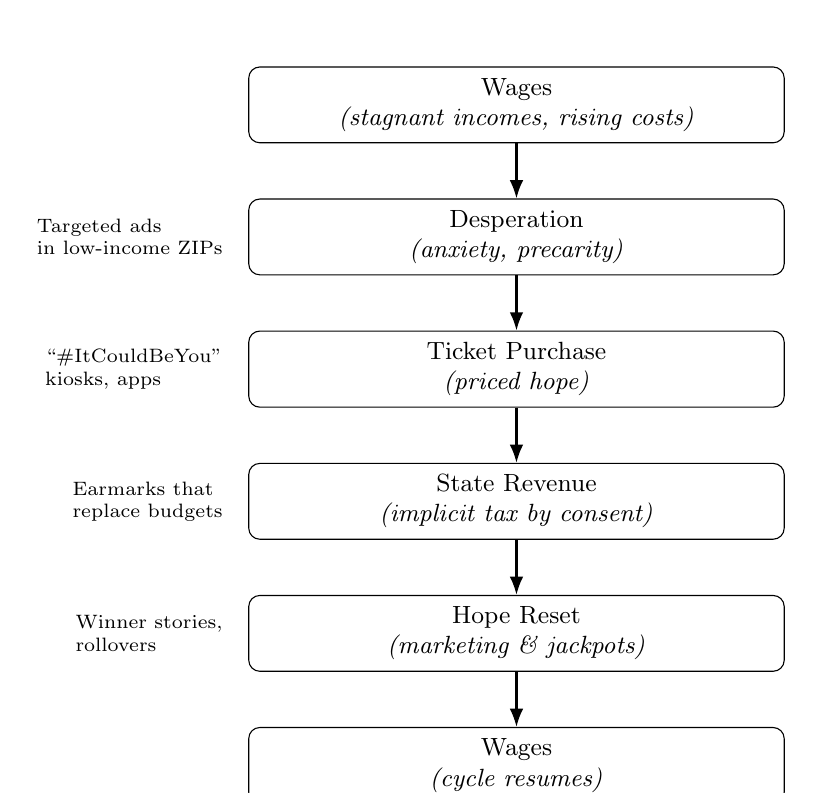
\begin{tikzpicture}[
  box/.style={draw, rounded corners, align=center, minimum width=6.8cm, inner sep=4pt},
  arrow/.style={-Latex, thick},
  every node/.style={font=\small},
  node distance=7mm
]
\node[box] (wages1)      {Wages \\ \textit{(stagnant incomes, rising costs)}};
\node[box, below=of wages1] (despair) {Desperation \\ \textit{(anxiety, precarity)}};
\node[box, below=of despair] (ticket)  {Ticket Purchase \\ \textit{(priced hope)}};
\node[box, below=of ticket] (revenue) {State Revenue \\ \textit{(implicit tax by consent)}};
\node[box, below=of revenue] (hope)    {Hope Reset \\ \textit{(marketing \& jackpots)}};
\node[box, below=of hope] (wages2)     {Wages \\ \textit{(cycle resumes)}};

\draw[arrow] (wages1) -- (despair);
\draw[arrow] (despair) -- (ticket);
\draw[arrow] (ticket) -- (revenue);
\draw[arrow] (revenue) -- (hope);
\draw[arrow] (hope) -- (wages2);

% side notes, tight to avoid margin issues
\node[align=left, font=\scriptsize, anchor=east, xshift=-2mm] at (despair.west)
  {Targeted ads\\ in low-income ZIPs};
\node[align=left, font=\scriptsize, anchor=east, xshift=-2mm] at (ticket.west)
  {“\#ItCouldBeYou”\\ kiosks, apps};
\node[align=left, font=\scriptsize, anchor=east, xshift=-2mm] at (revenue.west)
  {Earmarks that\\ replace budgets};
\node[align=left, font=\scriptsize, anchor=east, xshift=-2mm] at (hope.west)
  {Winner stories, \\ rollovers};

\end{tikzpicture}
\caption{The Lottery Feedback Loop — how stagnant wages and precarity are converted into state revenue via “priced hope,” sustaining a cycle of voluntary taxation and renewed belief.}
\label{fig:lottery-feedback}
\end{figure}

%\include{chapters/ch25.3}
\chapter{Give Caesar What Is Due to Caesar: The Commerce of Collapse}
\label{ch:25.3}
% --- 1500–2700 word manifesto chapter ---
% Use "The Great Hollowing" as the central analytic thread.

“Render unto Caesar the things that are Caesar’s.”  
The phrase once described the boundary between power and conscience—between the material order of the state and the moral order of the soul.  
In the twenty-first century that boundary has disappeared.  Caesar now collects both tribute and belief.  
Taxes are paid not only in currency but in attention, desire, and despair.  
Homelessness, addiction, pornography, and crime have become new forms of revenue, the raw materials of an economy that profits from social ruin.  
This is the twenty-fifth movement of \textbf{The Great Hollowing}: the monetization of collapse.

Modern governance has discovered that dysfunction can be managed as efficiently as production once was.  
Where industry once employed hands, bureaucracy now employs suffering.  
Every crisis feeds a chain of intermediaries—contractors, NGOs, insurers, pharmaceutical suppliers, data vendors—each extracting value from the administration of misery.  
The homeless are not a failure of policy; they are a business model.  
The addict is not a patient but a recurring customer.  
The criminal is not a tragedy but a statistic sustaining budgets and surveillance.  
Caesar has found a way to tax the ruins of his own empire.

\textbf{The Great Hollowing} manifests here as the moral outsourcing of responsibility.  
Compassion is delegated to programs; guilt is laundered through donations.  
Citizens tolerate decay because it circulates wealth upward.  
Every encampment justifies a new grant; every overdose sustains a new pharmaceutical subsidy.  
The welfare state and the market state merge into one organism that feeds on dependence while advertising care.  
Where charity once sought to heal, policy now seeks to manage.  
The bureaucrat’s success is measured not by resolution but by continuity.

The streets of every great Western city bear witness.  
Tents line sidewalks beneath digital billboards selling luxury watches and cryptocurrencies.  
An economy that can deliver groceries in fifteen minutes cannot house its own citizens.  
This contradiction is not accidental; it is the physical architecture of \textbf{The Great Hollowing}.  
When shelter becomes speculation, when medicine becomes subscription, when dignity becomes data, the body itself turns into collateral.

Addiction is the most profitable dependency ever engineered.  
Pharmaceutical companies convert pain into dividends; tech platforms convert loneliness into engagement; pornography converts intimacy into endless scroll.  
Each industry promises relief while deepening the void that sustains it.  
Desire is mined like ore: extracted, refined, and resold.  
The addict’s suffering is predictable, and predictability is profitable.  
Caesar, once content with tribute in gold, now collects dopamine.

The pornography of the digital age no longer hides behind shame; it brands itself as freedom.  
What was once vice is now monetized autonomy.  
Algorithms study arousal the way economists study demand, adjusting fantasy to demographic.  
Each click refines the product, narrowing the distance between stimulation and surrender.  
Desire becomes data, data becomes capital, and capital feeds the same systems that preach liberation while enforcing dependency.  
The citizen mistakes exposure for empowerment, mistaking infinite availability for intimacy.  
Freedom dissolves into frictionless consumption.

Crime itself becomes an input.  
Prisons, private security, and predictive-policing software transform chaos into budgetary necessity.  
The perpetual crisis of order guarantees contracts and campaigns.  
The cycle is immaculate: deprivation breeds crime, crime justifies control, control creates jobs, and jobs maintain deprivation.  
Caesar’s balance sheet now includes every broken window and every unhealed wound.  
Each act of violence is another invoice paid by the taxpayer and cleared by the market.

And through it all, the rhetoric of empathy persists.  
Governments speak of “harm reduction,” corporations of “community initiatives,” foundations of “inclusive futures.”  
The vocabulary of virtue conceals an economy of extraction.  
To question the arrangement is to invite accusations of cruelty, yet the true cruelty lies in perpetuation.  
When every evil is repackaged as a “challenge,” no reform is necessary.  
The wound must remain open for the healer to stay employed.

\textbf{The Great Hollowing} here reaches theological depth: sin without sinners, guilt without repentance, mercy without redemption.  
The moral economy has inverted itself.  
Where the poor were once seen as victims of injustice, they are now treated as assets of compassion—resources for the industries of care, imagery for the fundraising brochure, metrics for the quarterly report.  
Salvation has been nationalized; redemption outsourced.

\begin{tcolorbox}[
  title=\textbf{Economy of Misery},
  colback=white,
  colframe=black,
  fonttitle=\bfseries,
  top=0.5mm,
  bottom=0.5mm,
  left=3pt,
  right=3pt,
  before skip=4pt,
  after skip=6pt,
  arc=1mm,
  boxrule=0.4pt
  ]
\setlength{\itemsep}{1pt}
\begin{itemize}
  \item Every homeless person generates thousands in “service spending” per year.  
  \item Each incarceration supports a private industry of suppliers and data brokers.  
  \item Pharmaceutical profits rise in direct proportion to diagnosed despair.  
  \item Digital addiction is monetized twice—first by the platform, then by the therapist.  
  \item The more society decays, the more its GDP appears to grow.  
\end{itemize}
\end{tcolorbox}

Who benefits?  The same class that benefits from every other stage of the hollowing:  
the managers of crisis, the investors of despair, the bureaucrats of benevolence.  
The poor man pays for his own surveillance; the addict funds his own cure; the taxpayer finances his own degradation.  
Caesar collects all sides of the transaction.  
He has no need for armies; he has algorithms and contracts.  
His empire expands not by conquest but by compassion.  

Meanwhile, the middle class watches through screens, reassured that every misery is being “addressed.”  
The spectacle of suffering becomes a civic ritual—a nightly reminder that the system still functions, because someone, somewhere, is worse off.  
Outrage serves as entertainment; empathy as subscription.  
To give Caesar what is due now means to surrender outrage itself, to tithe one’s conscience to the bureaucracy of virtue.

The cycle is almost perfect: \\ 
1. Society produces despair. \\ 
2. Despair produces revenue. \\ 
3. Revenue sustains the institutions that preserve despair. \\ 
Only collapse can break it, and collapse itself has become profitable.

\begin{figure}[htbp]
\centering
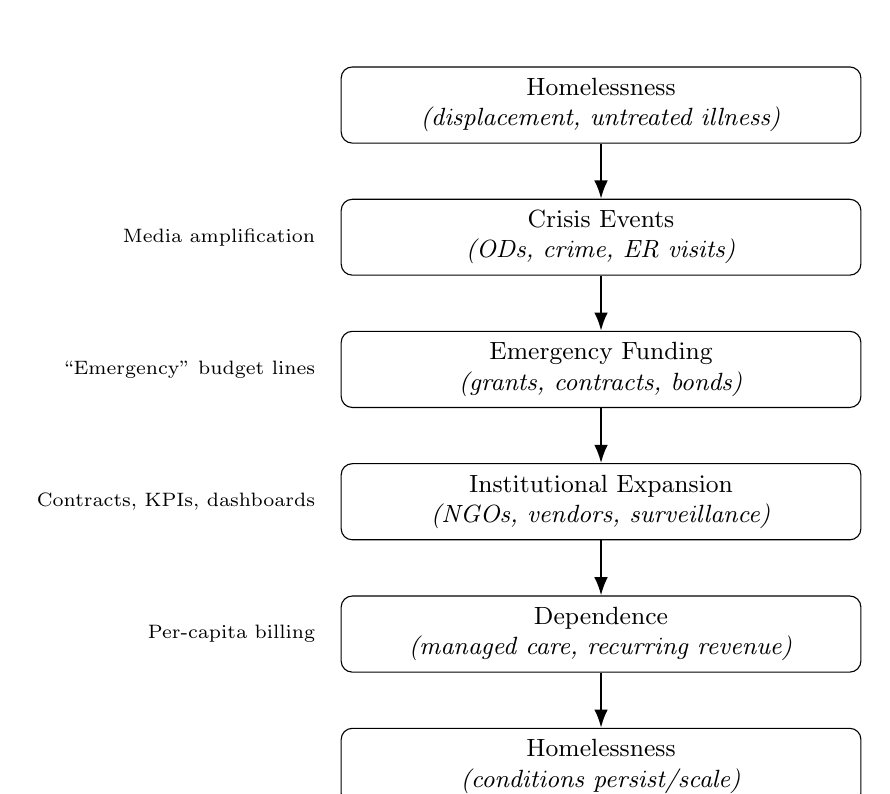
\begin{tikzpicture}[
  box/.style={draw, rounded corners, align=center, minimum width=6.6cm, inner sep=4pt},
  arrow/.style={-Latex, thick},
  every node/.style={font=\small},
  node distance=7mm
]
\node[box] (homeless1) {Homelessness \\ \textit{(displacement, untreated illness)}};
\node[box, below=of homeless1] (crisis) {Crisis Events \\ \textit{(ODs, crime, ER visits)}};
\node[box, below=of crisis] (funding) {Emergency Funding \\ \textit{(grants, contracts, bonds)}};
\node[box, below=of funding] (institution) {Institutional Expansion \\ \textit{(NGOs, vendors, surveillance)}};
\node[box, below=of institution] (depend) {Dependence \\ \textit{(managed care, recurring revenue)}};
\node[box, below=of depend] (homeless2) {Homelessness \\ \textit{(conditions persist/scale)}};

\draw[arrow] (homeless1) -- (crisis);
\draw[arrow] (crisis) -- (funding);
\draw[arrow] (funding) -- (institution);
\draw[arrow] (institution) -- (depend);
\draw[arrow] (depend) -- (homeless2);

% subtle side notes (remove if tight on space)
\node[align=left, font=\scriptsize, anchor=east, xshift=-2mm] at (crisis.west)
  {Media amplification};
\node[align=left, font=\scriptsize, anchor=east, xshift=-2mm] at (funding.west)
  {“Emergency” budget lines};
\node[align=left, font=\scriptsize, anchor=east, xshift=-2mm] at (institution.west)
  {Contracts, KPIs, dashboards};
\node[align=left, font=\scriptsize, anchor=east, xshift=-2mm] at (depend.west)
  {Per-capita billing};

\end{tikzpicture}
\caption{Cycle of Despair — how unmanaged homelessness converts into crisis, activates funding, grows institutions, and re-produces dependence, closing the loop.}
\label{fig:cycle-despair}
\end{figure}

\textbf{The Great Hollowing} therefore concludes its moral descent here—in the discovery that evil no longer needs intent.  
It only needs incentives.  
When vice yields dividends and virtue yields none, the outcome is certain.  
Caesar no longer demands worship; he provides it.  
His temples are hospitals, his hymns are advertisements, his altar is the screen.  
And the people, weary and willing, render unto him not their souls, but something far more valuable—their despair, renewed weekly and indexed to inflation.

%\include{chapters/ch25.4}
\chapter{The Economy of Punishment: Crime, Safety, and the Prison Dividend}
\label{ch:25.4}
% --- 1500–2700 word manifesto chapter ---
% Use "The Great Hollowing" as the central analytic thread.

A society reveals its soul by what it chooses to cage.  
When the factory closes and the social contract collapses, the state does not rebuild—it incarcerates.  
The modern prison is not an institution of correction but an accounting system, a method of balancing moral deficit with fiscal surplus.  
It stands as the twenty-sixth movement of \textbf{The Great Hollowing}: the conversion of crime into capital.

For every social wound, a market emerges.  
Homelessness feeds the shelter industry, addiction feeds the pharmaceutical industry, and crime feeds the incarceration industry.  
What was once the failure of society is now a growth sector, a predictable stream of revenue for pension funds and private equity.  
Wall Street’s prison stocks trade on the arithmetic of despair.  
The more citizens fall through the cracks, the more dividends flow upward.  
Freedom is no longer a right—it is a lease.

\textbf{The Great Hollowing} manifests here in the transformation of punishment into portfolio.  
Once, law served order; now it serves yield.  
The judicial system functions as a supply chain: police provide input, courts process inventory, prisons manage storage, and investors collect rent on the lost years of human beings.  
The moral language of “safety” conceals a logistical operation worth billions.  
The state manufactures risk the way a factory once manufactured steel.

Crime itself becomes a state-managed asset class.  
Legislation expands its definition; enforcement ensures its production.  
Minor infractions—trespassing, unpaid fines, possession, loitering—sustain the pipeline.  
Each arrest triggers funding, justifies equipment budgets, and maintains the illusion of order.  
Meanwhile, the root causes—poverty, addiction, untreated trauma—remain unsolved by design.  
To eliminate them would collapse the economy of punishment.

Private prison corporations, publicly traded and heavily lobbied, describe their mission in euphemisms:  
“Public safety partnerships,” “community reintegration programs,” “secure housing solutions.”  
But behind the marketing lies a simple metric—occupancy rate.  
Their contracts often include “bed guarantees,” requiring states to keep prisons 90–95\% full or pay penalties.  
Freedom, therefore, becomes an inefficiency; liberation, a liability.  
Justice is not served; it is serviced.

\textbf{The Great Hollowing} deepens when salvation itself becomes subcontracted.  
Religious charities and corporate philanthropies enter the carceral system as vendors of redemption.  
The Salvation Army operates prison labor programs under the banner of rehabilitation.  
Faith-based initiatives provide chaplaincy, counseling, and “moral realignment” funded by the same state that profits from incarceration.  
The cycle is perfect: crime produces punishment, punishment produces profit, profit funds virtue.  
Caesar collects both sin and absolution.

To the taxpayer, it is sold as efficiency.  
To the investor, as opportunity.  
To the media, as reform.  
The language of compassion has been financialized: “justice reinvestment,” “second chances,” “smart on crime.”  
Each phrase conceals the same arithmetic—more bodies, more billing.  
The system does not fail; it performs exactly as designed.  
A single prisoner can generate between \$30,000 and \$70,000 per year in state contracts, medical fees, and administrative overhead.  
No factory in history has achieved such consistent margins.

The political genius of the prison economy lies in its moral camouflage.  
It claims to preserve “quality of life,” to protect the innocent from the dangerous.  
In truth, it preserves the illusion of control in a society that no longer controls its own decay.  
When inequality reaches intolerable levels, punishment becomes the substitute for governance.  
The poor are not rehabilitated; they are removed.  
The wealthy are not safer; they are simply unseen.

Wall Street’s role in this architecture is not peripheral—it is structural.  
Investment funds hold shares in CoreCivic, GEO Group, and Aramark.  
Banks securitize prison debt; insurance companies underwrite construction bonds; technology firms provide monitoring and data analytics.  
The prisoner becomes a dataset feeding predictive models that justify further policing and incarceration.  
It is an algorithmic ouroboros—society consuming itself to maintain the illusion of safety.

The language of reform only tightens the loop.  
“Alternatives to incarceration” translate to private monitoring contracts.  
“Rehabilitation programs” become platforms that track, score, and monetize compliance.  
Every reform becomes a new market niche.  
The system expands not despite reform but through it.  
Progress becomes a marketing category of punishment.

\begin{tcolorbox}[
  title=\textbf{The Prison Dividend},
  colback=white,
  colframe=black,
  fonttitle=\bfseries,
  top=0.5mm,
  bottom=0.5mm,
  left=3pt,
  right=3pt,
  before skip=4pt,
  after skip=6pt,
  arc=1mm,
  boxrule=0.4pt
  ]
\setlength{\itemsep}{1pt}
\begin{itemize}
  \item Every inmate represents recurring state and federal transfers to private operators.  
  \item “Bed guarantees” lock states into contracts irrespective of crime rates.  
  \item Prison labor generates billions annually at wages below \$1/hour.  
  \item Faith-based and nonprofit programs receive federal grants proportional to recidivism rates.  
  \item The illusion of safety underwrites municipal bonds and election campaigns.  
\end{itemize}
\end{tcolorbox}

To question this machinery is to be labeled “soft on crime.”  
But the true softness lies in the moral cowardice of a state that punishes symptoms to protect shareholders.  
Addiction is not treated; it is confined.  
Poverty is not relieved; it is criminalized.  
Despair is not healed; it is monetized.  
The citizen becomes raw material for an empire of redemption without redemption.

\textbf{The Great Hollowing} reaches its institutional apex here—where virtue, punishment, and profit merge.  
The same government that fails to prevent crime ensures that its failure pays dividends.  
The same corporations that outsource jobs overseas build prisons at home.  
The same faiths that preach forgiveness cash state checks to manage the damned.  
Caesar has learned to privatize sin.

And so the streets remain unsafe, not because of criminals, but because of policy.  
Fear becomes the social currency that justifies control.  
Every televised crime, every viral outrage, every act of random violence reinforces the message: safety requires obedience.  
The more society fractures, the more power consolidates.  
The citizen, exhausted by chaos, consents to surveillance, curfews, and censorship in exchange for the promise of peace.

But peace built on profit cannot last.  
A civilization that converts its own dysfunction into revenue eventually forgets how to live without it.  
The prisons grow fuller; the neighborhoods emptier; the balance sheets stronger.  
The state becomes both shepherd and wolf, guiding the flock toward its own slaughter, convinced that order has been restored.
\begin{figure}[htbp]
\centering
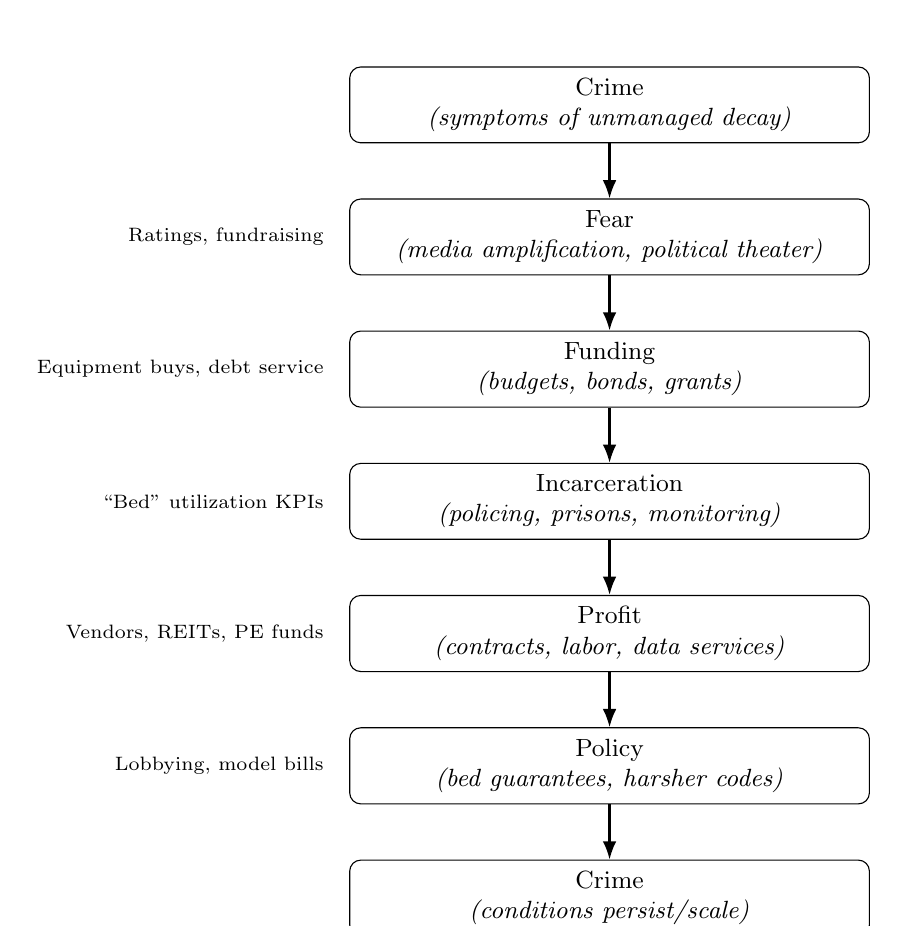
\begin{tikzpicture}[
  box/.style={draw, rounded corners, align=center, minimum width=6.6cm, inner sep=4pt},
  arrow/.style={-Latex, thick},
  every node/.style={font=\small},
  node distance=7mm
]
\node[box] (crime1) {Crime \\ \textit{(symptoms of unmanaged decay)}};
\node[box, below=of crime1] (fear) {Fear \\ \textit{(media amplification, political theater)}};
\node[box, below=of fear] (fund) {Funding \\ \textit{(budgets, bonds, grants)}};
\node[box, below=of fund] (incarc) {Incarceration \\ \textit{(policing, prisons, monitoring)}};
\node[box, below=of incarc] (profit) {Profit \\ \textit{(contracts, labor, data services)}};
\node[box, below=of profit] (policy) {Policy \\ \textit{(bed guarantees, harsher codes)}};
\node[box, below=of policy] (crime2) {Crime \\ \textit{(conditions persist/scale)}};

\draw[arrow] (crime1) -- (fear);
\draw[arrow] (fear) -- (fund);
\draw[arrow] (fund) -- (incarc);
\draw[arrow] (incarc) -- (profit);
\draw[arrow] (profit) -- (policy);
\draw[arrow] (policy) -- (crime2);

% optional side notes (delete if tight on margins)
\node[align=left, font=\scriptsize, anchor=east, xshift=-2mm] at (fear.west)
  {Ratings, fundraising};
\node[align=left, font=\scriptsize, anchor=east, xshift=-2mm] at (fund.west)
  {Equipment buys, debt service};
\node[align=left, font=\scriptsize, anchor=east, xshift=-2mm] at (incarc.west)
  {“Bed” utilization KPIs};
\node[align=left, font=\scriptsize, anchor=east, xshift=-2mm] at (profit.west)
  {Vendors, REITs, PE funds};
\node[align=left, font=\scriptsize, anchor=east, xshift=-2mm] at (policy.west)
  {Lobbying, model bills};

\end{tikzpicture}
\caption{The Prison Dividend Loop — how crime is converted into fear, fear into funding, funding into incarceration, incarceration into profit, profit into policy, and policy back into crime.}
\label{fig:prison-dividend-loop}
\end{figure}

The empire that calls itself free has rediscovered slavery—outsourced, automated, and moralized.  Caesar no longer needs legions; he has dividends.  
And the citizens, believing themselves protected, render unto him their fear.

% ==============================================================
% PART V — The Empire of Illusion
\part{The Empire of Illusion}

% \include{chapters/ch26.1}

% \include{chapters/ch26}
\chapter{Bolsheviks: From Revolution to Banker’s Evolution}
\label{ch:26.1}

Every revolution begins with the promise of liberation and ends with the perfection of control.  
The Bolshevik uprising of 1917 vowed to free humanity from the tyranny of capital.  
Instead, it reproduced the very architecture of centralization it sought to abolish.  
Across the ocean, another revolution—quiet, discreet, and financial—was taking place on Jekyll Island in 1910.  
Both revolutions, red and gold, would converge into a single managerial logic: the governance of humanity through systems.  
This is the twenty-sixth movement of \textbf{The Great Hollowing}—the transmutation of ideology into finance.

\section*{1. Two Revolutions, One Logic}

In Petrograd, the Bolsheviks replaced Tsarist privilege with Party hierarchy.  
In Washington, a handful of financiers replaced democratic volatility with monetary discipline.  
Each side imagined it was building a new order.  
Each ended by perfecting the old.  
The Soviet commissar and the Wall Street banker were opposite faces of the same impulse—to plan the unplannable, to manage the spontaneous, to control life through ledgers.

When Lenin’s forces seized the Winter Palace, they inherited a bureaucracy and merely changed its vocabulary.  
The aristocracy became the apparat.  
Gold reserves became Gosbank.  
The police became the Cheka.  
The people became production data.  
The dream of equality was reduced to arithmetic: the more perfectly the plan, the more perfectly humanity would obey it.  
What the revolution promised to abolish—debt, exploitation, abstraction—it simply nationalized.

Meanwhile, in the United States, an equally decisive centralization was unfolding in private form.

\section*{2. Jekyll Island and the Technocrats of Credit}

In November 1910, a private railcar departed Hoboken bound for Georgia.  
On board were Senator Nelson Aldrich (Republican power broker and father-in-law of John D. Rockefeller Jr.), Henry P. Davison of J.~P.~Morgan \& Co., Frank Vanderlip of National City Bank (Rockefeller’s bank), Paul Warburg of Kuhn, Loeb \& Co., and Benjamin Strong of Bankers Trust.  
The men traveled in secrecy under assumed names to Jekyll Island, a secluded resort owned by the Morgans and Rockefellers.  
Their mission was not to debate democracy but to design its replacement in the realm of money.  
Within a week, they had drafted the blueprint for the Federal Reserve System—an institution that would appear public but operate as private consensus.

Behind them stood the older dynasties of Europe: the Rothschild banking houses of London, Paris, and Frankfurt; the Warburgs of Hamburg; the Schiff family of Frankfurt and New York; the Barings of Britain; and the Lazards of France.  
Through Kuhn, Loeb \& Co., Jacob Schiff and Paul Warburg imported the Rothschild method—an international web of credit coordination masked by national rhetoric.  
Paul’s brother, Felix Warburg, remained in Europe, maintaining ties to the Bank of England and to the Rothschild–Baring–Morgan axis.  
Thus the Atlantic became an invisible balance sheet, with policy crossing the ocean faster than ships.

The Harriman industrial dynasty—railroads, steel, and mining—found in the Federal Reserve a perpetual guarantor of expansion.  
So too did Rockefeller’s Standard Oil empire, whose vast cash flows demanded a central mechanism for credit stabilization.  
To the public, this was modernization; to the initiates, it was monetized order.  
By 1913, the U.S. Congress passed the Federal Reserve Act.  
It would soon do for capitalism what Gosplan would later do for socialism: translate all human activity into numbers manageable by the few.

\section*{3. The Transatlantic Web of Centralization}

The early Federal Reserve governors—Benjamin Strong in New York, Warburg in Washington—were not revolutionaries but rationalizers.  
They shared Lenin’s faith in management, not Marx’s faith in man.  
Both believed chaos could be conquered through design.  
Both despised the uncertainty of human choice.  
The Bolshevik built the Five-Year Plan; the banker built the Open Market Committee.

From 1913 to 1930, the Federal Reserve and Gosbank evolved in eerie parallel.  
Both promised stability, both multiplied crises.  
The Soviet Union collectivized production to fight scarcity; the Federal Reserve collectivized credit to fight deflation.  
Each replaced reality with representation: paper for goods, statistics for hunger.  
By the time of Stalin’s purges and the Great Depression, the two systems—ideologically hostile—had become philosophically indistinguishable: command economies run by clerks of belief.

\textbf{The Great Hollowing} manifests here as the convergence of opposites.  
Capitalism and communism, once conceived as mortal enemies, both adopted the same core principle—central control masked as collective salvation.  
In Moscow, it was the dictatorship of the proletariat; in New York, the dictatorship of liquidity.  
Each system sought to domesticate uncertainty, to mechanize faith.

\section*{4. The Families Behind the Curtain}

The Rothschilds had mastered sovereign finance long before the twentieth century.  
From Waterloo to the Suez, their family network served as the central nervous system of European credit.  
Their model—private coordination, public dependence—became the template for modern banking.  
By the time of Jekyll Island, that model had been replicated through the Warburg–Schiff connection in New York, the Morgan banking syndicate, and the Rockefeller and Harriman industrial empires.  
These names were not conspirators; they were custodians of an emerging truth: power in the modern age resides not in armies, but in interest rates.

The Morgan empire, now institutionalized as J.~P.~Morgan \& Co., acted as the informal Treasury of the American Republic.  
Rockefeller’s National City Bank and Harriman’s Brown Brothers network financed everything from railroads to oil to early corporate globalization.  
The House of Rothschild coordinated European bonds; Kuhn, Loeb channeled German capital to American steel; the Warburgs advised the Bank of England on stabilization policy after World War I.  
By the 1920s, the Atlantic elites had achieved what Marx predicted but never imagined: a global bourgeoisie without borders.

The Bolsheviks, for all their rhetoric, mirrored this consolidation in political form.  
They destroyed private wealth but preserved private logic.  
In place of the invisible hand, they installed the invisible plan.  
The same impulse—control through abstraction—animated both Wall Street and the Kremlin.

\section*{5. From Central Planning to Central Banking}

The world wars only accelerated this convergence.  
War demanded coordination; coordination demanded credit.  
The Harriman network expanded into wartime shipping and postwar reconstruction; Morgan financed the Allied governments; the Rothschild and Lazard banks rebuilt Europe under the same principle: profit through planning.  
After 1945, the Bretton Woods institutions—the International Monetary Fund and the World Bank—formalized what had begun at Jekyll Island.  
Global finance became global governance.  
Where Lenin once dreamed of world revolution, the bankers achieved it in silent form.

Paul Warburg’s intellectual descendants—men like Montagu Norman of the Bank of England and Marriner Eccles of the Federal Reserve—believed they could steer civilization by adjusting the supply of money.  
By the late twentieth century, Alan Greenspan, Ben Bernanke, and their European counterparts operated as high priests of the invisible economy.  
They promised prosperity without production, stability without sacrifice.  
The numbers, like the slogans, always worked—until they didn’t.

\section*{6. From Commissars to Quantitative Easing}

In the Soviet Union, the dream of total coordination collapsed under the weight of falsified statistics.  
In the West, the same dream persisted under a new name: quantitative easing.  
Both systems relied on fabricated optimism; both punished dissent with economic exile.  
The Bolshevik gulag and the banker’s foreclosure were two versions of the same punishment—noncompliance with the plan.  
By the twenty-first century, the bureaucrat and the banker had fused into a single archetype: the algorithmic governor.

\textbf{The Great Hollowing} reaches its apogee when the system no longer needs belief—only participation.  
Citizens need not understand the plan; they only need to repay it.  
Democracy becomes consumer confidence; sovereignty becomes liquidity preference.  
The managers of modernity no longer govern people; they maintain flows.  
Human beings are treated as nodes in a balance sheet of stability.

\section*{7. The Return of the Hidden Kings}

Today’s central bankers—Christine Lagarde, Jerome Powell, Yi Gang—speak the same sanitized dialect once used by Party functionaries.  
Their press conferences echo Politburo briefings: “confidence,” “stability,” “transition.”  
The heirs of Morgan, Rockefeller, Warburg, and Rothschild still operate behind the symbols of progress.  
They no longer require secrecy; they have institutionalized it.  
The old families remain in foundations and funds—Rothschild \& Co., Brown Brothers Harriman, Rockefeller Capital, Warburg Pincus—each one a modern monastery of money, serene and opaque.

The Soviet Union collapsed visibly; the financial order persists invisibly.  
Its ideology is efficiency, its theology is liquidity, its moral law is growth.  
Yet beneath the polished reports, the same cracks appear.  
Productivity stagnates, inequality deepens, meaning evaporates.  
The same forces that hollowed out the socialist world now erode the capitalist one.  
The numbers no longer persuade.

\section*{8. The Reckoning of Abstraction}

What unites the Bolsheviks, the Warburgs, the Rothschilds, and the Harrimans is not conspiracy but conviction—that the world can be managed from the top down.  
Both Marx and Morgan believed that progress could be engineered.  
Both replaced the moral imagination of individuals with the mechanical precision of systems.  
This is the essence of \textbf{The Great Hollowing}: the evacuation of meaning from power, the substitution of algorithm for agency.

When this cycle ends—and it will—it will not be through another revolution of slogans but through the quiet rediscovery of reality.  
No decree, no policy rate, no committee can create value where trust has died.  
The lesson of Jekyll Island and the Winter Palace alike is simple:  
when man believes he can perfect the world through management, he builds the instruments of his own servitude.

And when the next crisis comes—as it always does—the world may at last remember what neither Lenin nor Warburg understood:  
that the wealth of a nation is not its currency but its conscience,  
and that no system, however intricate, can survive once its people stop believing in the arithmetic of salvation.

% \include{chapters/ch27}
\chapter{Infrastructure as Ideology}
\label{ch:27}
% --- TODO: 500--700 word chapter summary in manifesto--narrative tone.
% Use "The Great Hollowing" as the central analytic thread.

In every civilization, there comes a moment when words lose power and only structures remain.  
When the rhetoric of freedom, equality, or progress no longer persuades, architecture takes over as the true voice of ideology.  Roads, bridges, power grids, and fiber-optic cables become the new scriptures — silent but absolute.  Where philosophers once wrote constitutions, engineers now pour foundations.  This is the twenty-sixth movement of \textbf{The Great Hollowing}: the transmutation of belief into infrastructure.

Modernity once believed that ideas governed matter.  The Enlightenment built parliaments and universities to express its ideals in stone and paper.  But in the twenty-first century, matter governs ideas.  The design of a port, the latency of a network, or the width of a highway determines more about human destiny than any speech or law.  Infrastructure no longer follows ideology — it produces it.  Whoever builds the systems that connect the world controls the meanings that flow through them.

\textbf{The Great Hollowing} manifests here as the collapse of symbolic politics into physical logistics.  The promises of democracy are now routed through fiber optics owned by oligopolies; sovereignty is measured in bandwidth and supply-chain resilience.  Political revolutions are replaced by updates to infrastructure — pipelines of energy, data, and credit that shape the invisible geometry of dependence.  Power has ceased to be persuasive; it is infrastructural.

In the past, ideology sought legitimacy through persuasion.  Today, it achieves it through connectivity.  A regime need not convince its citizens when it can simply connect them — to jobs, to services, to feeds.  The illusion of participation replaces the substance of power.  As long as the network works, dissent remains abstract.  The new social contract is one of functionality: freedom redefined as uninterrupted service.

China understood this transformation earlier than most.  Its ideology of harmony is now encoded not in slogans but in infrastructure — railways that link continents, power grids that cross borders, 5G networks that carry both data and doctrine.  The Belt and Road Initiative is not merely a trade project; it is a metaphysical claim that order can be built physically, that global integration is a matter of engineering, not ideology.  Concrete becomes covenant.

The West, having hollowed out its own material base, struggles to match this logic.  Its infrastructures decay while its ideals remain pristine but inert.  It exports narratives, not networks.  Its democracies debate policies while outsourcing the cables that bind their economies.  In this new world, sovereignty belongs not to the most persuasive, but to the most infrastructural.  Power now flows through conduits, not constitutions.

Infrastructure, once seen as neutral, is in fact the most ideological space of all.  Every bridge encodes a worldview: what is connected, what is bypassed, what is controlled.  Every data center defines the boundary of visibility.  Every satellite constellation redraws the map of the possible.  The unspoken truth of globalization is that control no longer requires coercion; it requires connectivity.  The power that builds the road decides where everyone travels.

\textbf{The Great Hollowing} deepens as infrastructure becomes theology.  We no longer ask whether a system is just, only whether it is efficient.  Efficiency becomes the new moral good — the standard by which entire civilizations judge themselves.  The slogan of modern ideology is no longer “liberty” or “equality” but “seamless integration.”  The world worships the uninterrupted flow of goods, data, and desire.  Interruption itself becomes heresy.

This faith in infrastructure extends into the psychological realm.  People begin to model their inner lives after networks: optimized, responsive, always online.  Emotional resilience becomes “bandwidth,” social life “connectivity,” intellect “processing power.”  The metaphors of machines become the metrics of meaning.  The result is a civilization that no longer thinks about truth, only throughput.  The soul is replaced by signal strength.

China’s infrastructural state thus represents both an evolution and a warning.  It demonstrates that ideology can function without illusion — that belief can be built instead of preached.  Roads, dams, and satellites serve as sacraments of order, the physical proof of governance.  Citizens do not need to believe in the state; they inhabit it.  The system’s success is measured not in votes but in voltage.  Authority becomes ambient.

Meanwhile, in the West, infrastructure has become memory — a relic of industrial pride now privatized and neglected.  Bridges crumble, grids fail, cities flood.  The infrastructure that once symbolized collective destiny now exposes collective decline.  A civilization that refuses to maintain its foundations eventually doubts its own purpose.  The hollowing is not only economic but existential: when we stop building, we stop believing.

And yet, even as infrastructure dominates, it also reveals its fragility.  The more seamless the system, the more catastrophic its failure.  A broken pipeline, a severed cable, a blackout — each reminds humanity that its gods are mechanical.  The illusion of permanence cracks under entropy.  In that moment, ideology briefly reappears: the question of why returns to a world obsessed with how.

To escape the Great Hollowing, societies must reclaim infrastructure not as destiny but as dialogue.  Roads and grids must again serve human purpose, not replace it.  The challenge is not to dismantle networks but to rehumanize them — to see in every bridge the moral decision of who crosses, in every wire the ethical choice of what flows.  Infrastructure can bind or liberate, depending on whether it serves meaning or merely motion.

The final task of civilization, then, is to remember that the foundation is not the faith.  Concrete cannot replace conscience.  Fiber cannot transmit purpose.  A world of infinite connectivity without direction is only a more efficient emptiness.  \textbf{The Great Hollowing} warns that when ideology disappears into infrastructure, control becomes invisible — and freedom, obsolete.

The next age will be defined not by who has the largest network, but by who remembers why they built one at all.  
The true architecture of civilization is not its roads or data centers, but the moral imagination that decides where they lead.

% \include{chapters/ch28}
\chapter{Lessons from the East}
\label{ch:28}
% --- TODO: 500--700 word chapter summary in manifesto--narrative tone.
% Use "The Great Hollowing" as the central analytic thread.

Every civilization teaches, though few are willing to learn.  
The West once believed it had nothing left to study — that history had ended, that progress flowed in only one direction.  
But as its glass towers empty and its bridges rust, it begins to look eastward, toward a civilization that never stopped building.  
China’s rise is not just an economic event; it is a philosophical revelation.  
It reminds the world that power without purpose is noise, and that a society without discipline cannot endure its own freedom.  
This is the twenty-eighth movement of \textbf{The Great Hollowing}: the return of humility through contrast.

\bigskip

\textbf{The Abandonment of the Hellenic Light}

In the early seventeenth century the West departed from its own Hellenic enlightenment.  
The ancient Greek world had pursued \textit{arete} (ἀρετή) — excellence through balance of reason, virtue, and harmony.  
The citizen of the polis lived not for autonomy but for proportion; freedom existed within measure.  
Plato warned that when appetite rules, the soul fractures:  
\begin{quote}
\foreignlanguage{greek}{Ὅταν ἡ ἐπιθυμία βασιλεύῃ, τὸ λογιστικὸν δουλεύει.}  
(\textit{Republic}, IX, 580d)  
\end{quote}
“When desire becomes king, reason becomes its slave.”  
Yet modern Europe, in its rush toward liberation from all hierarchy, enthroned desire as destiny.  
The Enlightenment that might have fulfilled the dream of Athens became instead its inversion — a gospel of autonomy without harmony.  
In freeing the individual from order, it also freed greed from virtue.

Heraclitus had written,  
\begin{quote}
\foreignlanguage{greek}{ἦθος ἀνθρώπῳ δαίμων.}  
(\textit{Ethos anthrōpō daimon} — \textit{Fragment 119})  
\end{quote}
“Character is destiny.”  
But modern liberalism replaced character with choice.  
The polis became the market; dialogue became transaction.  
Aristotle’s vision of man as a political animal, ordered toward the common good, dissolved into the doctrine of the self-owner — the entrepreneur of existence.  
Thus began the long forgetting: the exile of metaphysics from politics and of meaning from freedom.  
\textbf{The Great Hollowing} did not start in the factory; it began in the soul.

\bigskip

\textbf{The Return of the Eastern Mirror}

While the West forgot proportion, the East preserved it in another key — not as metaphysics, but as morality.  
Confucius wrote:  
\begin{quote}
\begin{CJK*}{UTF8}{bsmi}
君子和而不同，小人同而不和。
\end{CJK*}  
(\textit{Analects}, 13.23)
\end{quote}
“The noble person seeks harmony without conformity; the petty person seeks conformity without harmony.”  
This single line encapsulates the Eastern antidote to Western dissolution.  
Harmony, not homogeneity, sustains civilization.  
Diversity is tolerated, but it must remain musical — dissonance within rhythm, not chaos without form.
\clearpage
Laozi offered the same insight in metaphysical form:  
\begin{quote}
\begin{CJK*}{UTF8}{bsmi}
人法地，地法天，天法道，道法自然。
\end{CJK*}  
(\textit{Daodejing}, 25)
\end{quote}
“Man follows the earth, earth follows heaven, heaven follows the Dao, and the Dao follows what is natural.”  
Order, in this vision, is not imposed but aligned.  
Where the West conquers nature, the East collaborates with it.  
Civilization is harmony with process, not mastery over it.

\textbf{The Great Hollowing} thus meets its opposite: a civilizational rhythm that values coherence over conquest.  
While Western economies fragmented into speculation, China turned finance into an instrument of material continuity.  
Its planners studied Wall Street not to imitate it but to subordinate it.  
Factories, ports, and data lines became expressions of a metaphysical duty — to hold chaos at bay by constructing coherence.  
Its skyscrapers are sermons in steel; its infrastructure a moral text written in concrete.

The East teaches that modernity need not destroy tradition.  
Confucius coexists with code, ritual with robotics.  
It accepts contradiction as continuity, seeing harmony not as stasis but as balance of opposites.  
The West, by contrast, wages war on its own memory — renouncing the sacred, deriding discipline, exalting novelty as salvation.  
In doing so, it gains innovation but loses identity.  
Progress without roots becomes velocity without vector.

Scale is the second lesson.  
Where Western liberalism celebrates the individual, Chinese modernity venerates the system.  
Its strength lies not in personal freedom but in coordinated purpose.  
To Western eyes this appears oppressive; to Chinese eyes it appears rational.  
A civilization of 1.4 billion cannot afford ideological anarchy.  
Order becomes compassion by necessity.  
\textbf{The Great Hollowing} reveals that freedom and order are not enemies — but imbalance between them is fatal.  
The East reminds us that structure is not tyranny; it is survival.

Time is the third lesson.  
Western capitalism lives by the quarter; Eastern planning lives by the century.  
This temporal asymmetry defines the global age.  
The West acts; the East endures.  
Its patience is strategic, not passive.  
Each decade of infrastructure investment, each silent reform, accumulates mass where Western economies chase momentum.  
The result is gravitational power — influence that requires no conquest.  
Empires once expanded by force; now they expand by supply chain.

Yet the East’s coherence carries its own peril.  
The same harmony that sustains unity can suppress truth.  
Innovation risks suffocation under the weight of conformity.  
A civilization built on collective duty may achieve stability, but at the cost of voice.  
Its success depends on whether it can preserve moral order without enforcing moral silence.  
\textbf{The Great Hollowing} warns that control, even when benevolent, hollows from within if it denies reflection.

Still, the deepest lesson from the East is metaphysical.  
It asserts that reality is relational — that existence is not a battlefield of wills but a web of responsibilities.  
This philosophy, implicit in Confucian ethics and explicit in the design of China’s modern economy, contrasts sharply with the Western cult of autonomy.  
To act is to affect, to own is to owe.  
Even the market, in its vast complexity, is a network of obligations.  
Harmony, not competition, is the equilibrium of the real.

From this, a global synthesis begins to glimmer.  
The East cannot remain purely material; the West cannot remain purely abstract.  
One must learn purpose, the other humility.  
The industrial Confucianism of the East must discover voice; the financial idealism of the West must rediscover substance.  
Only through this dialectic can the Great Hollowing be reversed.  
Civilization will heal when technology serves virtue and freedom remembers form.

The lesson is not that the East has triumphed, but that it has remembered something the West forgot: that civilization is not a race but a rhythm.  
Its measure is not speed but coherence — the alignment of power, principle, and purpose.  
The West, blinded by acceleration, mistook exhaustion for achievement.  
The East, moving slower but deeper, built a continuity that outlasts crisis.  
Its faith is not in perpetual motion, but in perpetual balance.

The future will belong to those who understand both.  
The next renaissance will not arise from dominance, but from synthesis — from East and West learning to trade not commodities but consciousness.  
When abstraction rediscovers the physical, and control rediscovers conscience, the hollowing will end.  
Until then, the East will continue to build while the West continues to explain — and the world will move to the rhythm of whoever still believes in the act of construction.

% \include{chapters/ch29}
\chapter{The New Industrial Confucianism}
\label{ch:29}
% --- TODO: 500--700 word chapter summary in manifesto--narrative tone.
% Use "The Great Hollowing" as the central analytic thread.

The West built its modernity on rebellion; the East, on order.  
In Europe, progress meant breaking with the past — dethroning kings, questioning gods, privatizing conscience.  
In China, progress meant continuity — harmonizing the new with the ancient, embedding the machine in the moral.  
Now, in the twenty-first century, as Western civilization drowns in abstraction, China reemerges not only as a factory, but as a philosophy.  
It revives Confucius as a technocrat, ancestor worship as industrial strategy, and hierarchy as a principle of efficiency.  
This is the twenty-seventh movement of \textbf{The Great Hollowing}: the resurrection of ethics as infrastructure.

The world once imagined that modernization required secularization.  
Yet China’s rise reveals something subtler — modernization through moralization.  
Factories, data centers, and high-speed trains coexist with temples, ancestral rituals, and classical aphorisms.  
The past is not abolished but algorithmically integrated.  
Where the West separates spirit from system, China fuses them.  
It builds an economy that speaks the language of Confucian virtue: discipline, harmony, respect for hierarchy, and devotion to collective purpose.

At the heart of Confucianism lies the concept of \textit{li} (\CJKtrad{禮}) — ritual propriety, the choreography of society.
  
In the industrial age, \textit{li} reappears as protocol, regulation, and standardization.  
Factories run not on freedom but on ritualized precision.  
Workflows replace ceremonies; timetables replace temples.  
The obedience once demanded by moral order is now demanded by technical necessity.  
To maintain the flow of production is to maintain cosmic balance.  
\foreignlanguage{greek}{κόσμος} (order) has become logistics.

\textbf{The Great Hollowing} manifests here as a paradox: a civilization that preserves meaning through conformity.  
The individual disappears into the machine, yet feels ennobled by its purpose.  
Work becomes a moral act, production a form of piety.  
This moralization of labor grants China a coherence that the West has lost.  
Where Western workers view discipline as alienation, their Eastern counterparts perceive it as virtue — a means of fulfilling one’s role within the collective harmony.

The Chinese state exploits this moral heritage with precision.  
Its ideology does not rely on divine authority or democratic legitimacy, but on continuity — the promise that order itself is benevolence.  
Confucian ethics provide the emotional grammar of the modern technocracy: the leader as father, the bureaucrat as scholar, the citizen as dutiful child.  
To obey is not submission but participation in the collective harmony.  
Control is framed as care; hierarchy as compassion.  
The algorithm becomes the new \textit{Mandate of Heaven}.

This moral structure turns efficiency into virtue.  
In the West, efficiency is mechanical — the reduction of waste.  
In the Chinese context, it becomes ethical — the reduction of discord.  
Infrastructure serves not only to move goods but to stabilize relationships.  
The high-speed rail line and the Confucian proverb fulfill the same function: the unification of distance into order.  
China’s industrialization thus proceeds with moral aesthetics — factories as temples of harmony, networks as extensions of family.

\textbf{The Great Hollowing} deepens as ideology becomes etiquette.  
Western societies shout their values; China performs them.  
The moral code is silent, embedded in gesture, rhythm, and architecture.  
The factory foreman quoting Confucius is not hypocritical but literal:  
“To govern is to rectify names” (\textit{Analects}, XIII.3).  
Each component must do what it is named to do.  
Precision is morality.  
A screw out of place is a sin against order.

Yet this Confucian revival is not pure tradition — it is adaptation.  
Ancient virtue now serves industrial continuity.  
Harmony is used to justify surveillance; loyalty to legitimize conformity.  
The same ethics that once restrained power now stabilize it.  
The ruler’s benevolence becomes algorithmic paternalism; the citizen’s filial piety becomes data compliance.  
The moral order survives by reversing its polarity: it protects authority from scrutiny rather than the people from excess.

Still, beneath the hierarchy lies a philosophical coherence that the West secretly envies.  
In its worship of autonomy, the West shattered the very idea of collective purpose.  
Its democracies produce citizens without cohesion, markets without meaning.  
China, by contrast, retains the metaphysical confidence of a civilization that never doubted its continuity.  
It does not ask whether it is modern — it simply absorbs modernity into its ancient grammar.  
To build is to honor the ancestors; to plan is to preserve the harmony of the world.

This sense of time grants China an advantage beyond economics.  
Its development model is patient, cyclical, reflective.  
While Western markets live in quarterly frenzy, Chinese planning spans dynastic decades.  
Infrastructure projects begin as moral duties rather than speculative gambles.  
A dam or railway is not merely an investment; it is a statement about destiny.  
History is not progress; it is restoration.  
Each generation repairs what the previous left incomplete.

The cost of this model, however, is internal silence.  
Harmony suppresses dissent as noise.  
Critique is seen as contamination, individuality as entropy.  
The social order achieves peace by neutralizing unpredictability.  
In such a system, innovation must disguise itself as loyalty, and rebellion must masquerade as refinement.  
\textbf{The Great Hollowing} warns that when virtue becomes performance, ethics turns into protocol — the soul becomes an interface.

Yet even this industrial Confucianism contains an echo of wisdom.  
It reminds a fragmented world that civilization cannot endure without moral rhythm.  
To build is not enough; one must build with purpose.  
To produce is not progress unless it sustains harmony.  
China’s moral-industrial synthesis, for all its dangers, exposes the vacuum at the heart of the Western machine: a system without a story.  
Confucius, reinterpreted for the digital age, offers at least a narrative of order — flawed, rigid, but coherent.

Perhaps the future will not belong to the libertarian coder or the technocratic planner, but to whoever rediscovers virtue as architecture — the discipline that binds freedom to form.  
When machines obey harmony and markets rediscover moderation, the machine may yet become moral again.  
Until then, the world remains divided between two hollows: the West’s void of meaning and the East’s void of voice.

\textbf{The Great Hollowing} continues not because humanity has lost faith, but because it has divided it — between the algorithm and the ancestor, the profit and the principle.  
The task ahead is to reunite them.  
For only a civilization that can build both materially and morally will endure the century that follows.

% \include{chapters/ch30}
\chapter{Return of the Empire in the East: A New Life is Born — The Third Rome}
\label{ch:30}
% --- TODO: 500--700 word chapter summary in manifesto--narrative tone.
% Use "The Great Hollowing" as the central analytic thread.

Every decline summons its counterforce.  
As the West dissolves into abstraction—financial, digital, and ideological—the East turns again toward substance, toward memory, toward order.  
What was once dismissed as archaic has begun to reassert itself as the only remaining source of coherence.  
This is the thirtieth movement of \textbf{The Great Hollowing}: the re-materialization of civilization in the East, the birth of a new empire rising from the ruins of exhausted modernity.

\section*{1. The Empty West and the Waiting East}

The West, having conquered the world, has lost the power to believe in itself.  
Its democracies have become procedural, its markets self-referential, its art ironic, its churches empty.  
Freedom, once the glory of Athens and the promise of Jefferson, has devolved into consumption and spectacle.  
In abandoning substance for symbols—law for litigation, truth for narrative, matter for image—the West has hollowed itself into impotence.  
It no longer exports goods or ideas, only software and slogans.

Meanwhile, in the East, the memory of history remains unbroken.  
China, India, Russia, Iran—civilizations older than modernity itself—are not merely rising economically; they are remembering metaphysically.  
They are rediscovering what the Enlightenment forgot: that a civilization cannot stand on reason alone, and that meaning must be embodied in ritual, hierarchy, and purpose.  
The East is not inventing a future; it is reclaiming continuity.

\section*{2. The Meaning of the Third Rome}

In the year 1510, the monk Philotheus of Pskov wrote to the Grand Duke of Moscow:  
\textit{“Two Romes have fallen, the third stands, and there will be no fourth.”}  
He spoke not of political conquest but of spiritual inheritance—of the belief that divine order, abandoned by the Latin West, had migrated eastward.  
For centuries, that prophecy slept, mocked by reformers and rationalists.  
But as the twentieth century’s empires collapsed into managerial nihilism, the old idea stirred again.

The “Third Rome” is more than a geopolitical claim; it is a metaphysical one.  
It asserts that civilization must once again be governed by meaning rather than markets, by sacred proportion rather than statistical performance.  
It envisions sovereignty not as domination but as stewardship—a unity between state, culture, and spirit.  
In this sense, Moscow’s return to empire, Beijing’s doctrine of harmony, Tehran’s theology of resistance, and Delhi’s civilizational revival are all variations of the same phenomenon: the reemergence of rooted power.

\section*{3. From Collapse to Consolidation}

The twentieth century broke the world into competing ideologies; the twenty-first is reassembling it into civilizations.  
The East watched as Western liberalism consumed itself in contradictions—rights without responsibilities, wealth without production, speech without truth.  
When the Soviet Union fell, many believed history had ended.  
Instead, it merely changed direction.  
What collapsed was not Russia but Marxism; what survived was the deeper instinct for order—the belief that chaos is not freedom but decay.

Russia, in particular, represents this civilizational counterweight.  
Where the West celebrates the self, Russia remembers the collective.  
Where the West worships efficiency, Russia venerates endurance.  
Its rebirth is not merely nationalist but spiritual—a refusal to let the human soul be reduced to data.  
Its architecture, iconography, and literature carry the same message: that the sacred cannot be privatized.  
The so-called “authoritarianism” of the East is, in part, a reaction against the libertinism of the West—a defense of form against formlessness.

\section*{4. China and the Return of Civilizational Planning}

China’s rise is not a fluke of capitalism; it is the culmination of 2,000 years of administrative philosophy.  
Where the Western corporation serves shareholders, the Chinese state serves continuity.  
Confucius taught that the highest form of governance is not control but harmony:  
\textit{“To govern by virtue is like the North Star: it remains in its place while all the other stars turn toward it.”}  
(\textit{Analects} 2:1).  
Modern China, for all its surveillance and technocracy, operates within this ancient logic—the belief that social order precedes individual liberty.

Through the Belt and Road Initiative, China has reinterpreted empire as infrastructure.  
Railways, ports, and power lines have replaced colonies and crusades.  
Its ambition is not territorial conquest but economic geometry—a web of material interdependence that binds continents without firing a shot.  
While Western powers debate ideology, Beijing lays cables.  
While Washington speaks of “values,” Shanghai builds the servers that carry them.  
Power has migrated from parliaments to ports.

\section*{5. India, Iran, and the Multipolar Spirit}

India’s revival is civilizational rather than political.  
The rediscovery of Vedantic philosophy, the resurrection of Sanskrit learning, the assertive pride in ancient identity—all signal a shift from imitation to self-definition.  
Like Russia and China, India’s strength lies in continuity; it has survived every empire because it remembers what the West has forgotten—that truth is not an invention but a discovery.

Iran, too, embodies this return to sacred politics.  
Despised by the secular West for its theocracy, it nonetheless preserves a coherence that technocratic regimes cannot replicate.  
Its notion of sovereignty is theological: the ruler is accountable not to markets but to divine order.  
In a world where democracies vote for oblivion, Iran insists that destiny requires discipline.  
It may be authoritarian, but it is not hollow.

Together, these civilizations represent what might be called the *multipolar metaphysic*:  
a world in which power is not centralized in ideology but distributed through memory.  
Each draws from its own archive of meaning to resist the managerial nihilism of global finance.  
Each refuses to confuse convenience with civilization.

\section*{6. The Third Rome and the Western Void}

For the West, the rise of the East feels like betrayal.  
It sees authoritarianism where others see coherence; it mistakes rootedness for regression.  
But beneath the rhetoric lies envy.  
The East still believes in destiny; the West believes only in process.  
The East still honors the sacred; the West commodifies it.  
The East still builds monuments; the West debates zoning laws.  
The difference is not moral but metaphysical: one side remembers, the other rationalizes.

The prophecy of the Third Rome, in this sense, is not about geography but about gravity.  
It signifies the re-centering of civilization in places where meaning has not yet been erased.  
It is the pendulum swing of history correcting imbalance.  
Where the West hollowed out matter in pursuit of efficiency, the East fills the void with form.  
The world is rediscovering that order—whether Confucian, Orthodox, or Islamic—is not oppression but architecture.

\section*{7. The Spiritual War Beneath the Economic One}

The conflict between West and East is often described in terms of resources or ideology.  
In truth, it is metaphysical.  
It is a war between two conceptions of reality: one that views the world as a machine, and one that sees it as a living organism.  
The West seeks to manage; the East seeks to harmonize.  
The West measures progress by velocity; the East measures it by balance.  
The Great Hollowing began when matter lost meaning; the new empire of the East begins by reuniting them.

The resurrection of sacred art, the return of public ritual, the reverence for ancestors and land—these are not political gestures but ontological ones.  
They reassert that the material world is not raw material but divine manifestation.  
In the West, the cathedral became a museum; in the East, it remains a temple.  
That difference explains more than any economic chart.

\section*{8. The Eurasian Synthesis}

The Third Rome is not an isolated polity; it is the seed of a larger Eurasian synthesis.  
From the Arctic ports of Murmansk to the harbors of Gwadar and the railways of Xi’an, a new geography of integration is forming.  
Pipelines replace crusades; energy replaces ideology.  
The Eurasian landmass—once divided by empires—is coalescing into a civilization of interdependence rooted in material infrastructure and spiritual continuity.  
This synthesis challenges not only Western hegemony but the very assumption that modernity must be liberal.

Its cultural vision is post-liberal yet not anti-modern: technological progress guided by moral restraint, sovereignty balanced by solidarity.  
It does not reject science or trade; it reorders them beneath meaning.  
Its message to the world is not “freedom” but “form.”  
And in an age of exhaustion, form is beginning to triumph.

\section*{9. The Mirror for the West}

To the Western observer, the rise of this new empire may appear threatening.  
But history often sends correction in the guise of competition.  
The West’s decline is not irreversible; it is instructive.  
The East’s resurgence is not domination; it is reminder.  
It reminds the world that culture cannot live on consumption, that freedom without faith is noise, and that technology without transcendence is tyranny.

The lesson of the Third Rome is not that the East is destined to rule, but that civilization must once again be ruled by something higher than profit.  
The empire that endures will not be the richest, but the one most faithful to meaning.  
It will not worship speed, but proportion.  
It will not abolish tradition, but renew it.  
It will not enslave the world to machines, but teach machines to serve the world.

\section*{10. A New Life is Born}

Out of the ruins of managerial civilization, a new principle of order is taking shape.  
It is neither communist nor capitalist, neither Eastern nor Western—it is human and sacred.  
It recognizes that the earth is not a platform but a home, that time is not an investment but a covenant.  
It seeks not dominance but dignity.  
This is the spirit of the Third Rome: a civilization reborn not through ideology but through remembrance.

The West once believed it could save the world by exporting its abstractions.  
The East now saves itself by re-rooting in the real.  
From Byzantium’s ashes, from the monasteries of Mount Athos to the cathedrals of Moscow, from the ports of Shanghai to the temples of Varanasi, a single idea rises again:  
that truth cannot be digitized, that civilization must be incarnate, and that every empire built on illusion will, at last, kneel before the weight of the world.

\textbf{The Great Hollowing} began when the world forgot where it stood.  
The Third Rome begins where the ground is remembered again.

% \include{chapters/ch31}
\chapter{Re-rooting the Economy in Reality}
\label{ch:31}
% --- TODO: 500--700 word chapter summary in manifesto--narrative tone.
% Use "The Great Hollowing" as the central analytic thread.

An economy without matter eventually forgets what it costs to exist.  
When value detaches from substance, production becomes performance and consumption becomes creed.  
A civilization that once turned clay into temples now turns promises into portfolios.  
The balance sheet has replaced the workshop as the measure of worth.  
This is the thirty-first movement of \textbf{The Great Hollowing}: the severing of economy from reality—and the first gesture toward its repair.

\bigskip

For most of human history, wealth had weight.  
Grain filled granaries; stone built walls; gold could be held.  
The rhythms of labor and season grounded exchange in the physical world.  
Even error was tangible: a bad harvest, a cracked tool, a collapsed bridge.  
Reality imposed discipline.  
But in the age of financialization, the real became optional.  
Derivatives multiplied faster than crops, and code replaced craft.  
Growth no longer described the expansion of production but the inflation of symbols.  
A civilization addicted to abstraction mistook liquidity for life.

\textbf{The Great Hollowing} began when value ceased to correspond to creation.  
Once, the worker shaped matter into meaning; now, the market shapes meaning without matter.  
The price of a company rises on narratives rather than goods, and entire fortunes rest upon the expectation of expectation.  
Capital circulates like blood with no body to sustain.  
The economy, once an ecosystem, has become an echo chamber.

To re-root the economy in reality is therefore not nostalgia—it is survival.  
It means restoring proportion between symbol and substance, between credit and craft.  
It demands that production regain primacy over performance, and that finance return to its original role: service to creation, not substitution for it.

\bigskip

The first step is philosophical.  
Reality must again become the measure of value.  
Aristotle distinguished between "chrematistics"—the art of acquiring money—and "oikonomia"—the stewardship of the household.  
Modern economics confused the two, worshipping circulation over sufficiency.  
To re-root is to remember that economy is not an abstraction of exchange but a discipline of care: the tending of material life so that spirit may flourish within it.  
\begin{quote}
\foreignlanguage{greek}{ἡ φύσις οὐθὲν μάτην ποιεῖ.}  
(\textit{Physics}, II.8)  
\end{quote}
“Nature does nothing in vain.”  
An economy that consumes without creating violates both reason and rhythm.

The second step is structural.  
Production must again precede speculation.  
Industries of substance—energy, agriculture, infrastructure, manufacturing—must reclaim the dignity lost to the finance sector’s theater of perpetual motion.  
Innovation must be judged not by valuation rounds but by its capacity to sustain life and labor.  
A company that cannot feed, shelter, heal, or educate is not productive; it is performative.  
The test of progress is no longer speed but solidity.

The third step is moral.  
Consumption must regain conscience.  
Every purchase is a vote for the world one wishes to inhabit.  
The convenience economy, built on invisible suffering and planetary depletion, externalizes its costs into silence.  
To buy without awareness is to participate in disappearance.  
Re-rooting requires a new ethic of proximity: knowing who makes what we use, and what price reality pays for our comfort.  
True affordability includes accountability.

\textbf{The Great Hollowing} thrives on distance—between consumer and producer, manager and worker, shareholder and soil.  
Re-rooting collapses these distances.  
It replaces the anonymous global chain with the visible local circle, not as protectionism but as realism.  
Resilience is born from relation.  
A city that can grow its food, repair its tools, and harness its energy need not fear the tremors of abstraction.  
Sustainability is not an ideology; it is a geometry of proximity.

The fourth step is technological.  
Digital systems must descend from simulation back into service.  
Data can illuminate production but must not replace it.  
Artificial intelligence should assist material intelligence—the craftsman, the farmer, the scientist—not manage them.  
Technology that measures the world without touching it becomes theology without faith.  
Tools must again be extensions of hand and mind, not replacements for them.  
As Confucius warned,
\begin{quote}
\begin{CJK*}{UTF8}{bsmi}
名不正，則言不順；言不順，則事不成。
\end{CJK*}  
(\textit{Analects}, 13.3)
\end{quote}
“If names are not correct, speech will not accord with truth; if speech does not accord with truth, affairs cannot succeed.”  
So too in the digital age: when we call speculation “innovation” or extraction “growth,” disorder follows.

\bigskip

Re-rooting the economy also means re-imagining work.  
The labor of the future cannot be abstract labor.  
It must integrate thinking and making, automation and artistry.  
Every worker must again become a maker—whether of code, of care, or of culture.  
Pride will return not through salary but through substance.  
We will measure employment not by hours billed but by realities improved.  
When the craftsman and the coder are recognized as kin, the economy will once again resemble an organism rather than a machine.

The political implications are profound.  
Governments must cease treating GDP as theology and begin measuring vitality: the health of soil, the stability of families, the coherence of communities.  
Policy must favor durability over growth, quality over quantity, and autonomy over dependency.  
Democracy itself must be re-anchored in the tangible—local production, regional self-reliance, national purpose.  
Sovereignty begins where material competence returns.

\textbf{The Great Hollowing} will not end through collapse but through correction—through countless acts of reconnection between idea and object.  
A repaired chair, a rebuilt factory, a restored wetland—each is a gesture of metaphysical repair.  
Reality re-enters the economy one act of attention at a time.  
The invisible hand must rediscover the visible world.

\bigskip

To re-root is ultimately to remember that economy is a form of ecology—the management of relationships between living and made things.  
When the flow of capital once again serves the flow of life, when production becomes participation, and when value once again means value to someone, the hollowing will end.  
The market will cease to be a mirror and become a medium: a space where reality is exchanged, not erased.

Civilization will not be saved by profit but by proportion.  
Its rebirth will not come from another innovation cycle, but from a renewed covenant with the physical.  
To work, to build, to repair—these are not nostalgic acts.  
They are the grammar of being made whole again.

When the hand meets the world and feels its weight, the illusion of infinity breaks.  
We remember that the earth is finite, that meaning is material, and that value, like virtue, must be embodied to be real.  
The economy will heal when it becomes once more a household—\textit{oikos}—and when humanity learns again that the foundation of wealth is not credit, but creation.

% \include{chapters/ch32}
\chapter{The Death of Pride in Work}
\label{ch:32}
% --- TODO: 500--700 word chapter summary in manifesto--narrative tone.
% Use "The Great Hollowing" as the central analytic thread.

Civilization begins not with words, but with hands.  
The first temple was built by touch, the first law carved by labor.  
For millennia, work was the grammar of being — the way humanity wrote itself into the world.  
The craftsman, the farmer, the builder, and the scholar each participated in creation; their pride came not from ownership, but from excellence.  
To work was to shape reality according to reason and beauty.  
But in the modern age, that covenant has broken.  
Work no longer reveals dignity; it disguises despair.  
This is the twenty-ninth movement of \textbf{The Great Hollowing}: the death of pride in work.

\bigskip

The ancients understood labor as moral art.  
In Greece, the sculptor sought not profit but perfection — to make marble reveal the divine.  
Plato described the just man as a craftsman of the soul, harmonizing reason and desire like a builder aligning columns with the sun.  
Aristotle wrote,  
\begin{quote}
\foreignlanguage{greek}{ἡ ἀρετὴ ἐν ἔργῳ τελεῖται.}  
(\textit{Nicomachean Ethics}, II.4)  
\end{quote}
“Virtue is perfected in action.”  
The worth of work lay not in what it produced but in what it refined within the worker.  
\clearpage
Even in Confucian thought, centuries later, labor was an extension of virtue.  
\begin{quote}
\begin{CJK*}{UTF8}{bsmi}
工欲善其事，必先利其器。
\end{CJK*}  
(\textit{Analects}, 15.9)
\end{quote}
“If a craftsman wishes to do good work, he must first sharpen his tools.”  
The lesson was moral, not technical: the tool was the self.

\textbf{The Great Hollowing} began when this moral equation inverted — when work ceased to express character and began to extract it.  
Industrialization mechanized the gesture; automation digitized the mind.  
The craftsman became operator, the operator became data point.  
As efficiency rose, intimacy with creation fell.  
The modern worker no longer knows the fruit of his labor; he monitors it through dashboards and graphs.  
The pride of making was replaced by the anxiety of maintaining.

Under corporate management, labor became simulation.  
Meetings replaced materials, procedures replaced precision.  
A century ago, the engineer signed his bridge; today, the employee signs a non-disclosure agreement.  
The work of the mind, once liberation from toil, has become its most refined prison — endless coordination detached from consequence.  
White-collar labor, draped in professionalism, is only the ghost of production.  
It performs meaning to conceal its absence.

\textbf{The Great Hollowing} thus entered the psyche.  
The modern worker is trained to confuse exhaustion with achievement.  
Productivity becomes morality, and overwork becomes proof of worth.  
But because the work produces nothing lasting, fatigue yields no pride — only emptiness.  
The worker becomes a participant in the ritual of motion, worshipping metrics that erase his humanity.  
This is not labor; it is liturgy without faith.

In the West, the moral collapse of work followed the financialization of the economy.  
Pride once derived from the tangible — a built structure, a repaired engine, a completed symphony.  
Now it derives from the intangible — valuation, reputation, digital reach.  
Value exists only as perception.  
As a result, meaning migrates from action to performance.  
The worker ceases to create and begins to curate.  
Each profession becomes theater, every role a brand.  
The craftsman becomes influencer; the product becomes presentation.

In the East, by contrast, pride in work still survives — but often through coercion rather than joy.  
Discipline and hierarchy sustain collective efficiency, yet individuality withers beneath obedience.  
The pride of the Chinese builder or Japanese engineer is genuine, but it is bounded by expectation.  
The Confucian virtue of diligence survives, yet it has become instrumentalized — a virtue employed to maintain productivity, not transcend it.  
The moral foundation remains, but it has been absorbed into the machine.  
The worker’s humility is praised, but his soul is unseen.

The modern ideology of work — both East and West — has forgotten its original purpose: to reveal the human capacity for meaning through making.  
Karl Marx, though often misread, understood this tragedy when he wrote of alienation: that labor, detached from creation, estranges man from himself.  
But today’s alienation is subtler — it wears a smile.  
The open office, the corporate slogan, the digital nomad all promise autonomy while delivering abstraction.  
Freedom has been outsourced to flexibility.  
No one belongs anywhere; everyone is available everywhere.

\textbf{The Great Hollowing} deepens because work now exists without witness.  
The maker once stood before his creation and saw himself reflected in it.  
The architect could touch his building; the farmer could eat his harvest.  
Now the worker’s product is invisible, diffused through global networks.  
The pride that once bound identity to effort dissipates into screens and servers.  
To be productive today is to vanish into process.  
To finish is to forget.

And yet, beneath the automation and the emptiness, the human impulse to make endures.  
It survives in small rebellions — in the artisan who carves wood by hand, the coder who writes open-source for joy, the teacher who crafts meaning rather than metrics.  
These acts, though economically minor, are metaphysically immense.  
They restore the link between creation and consciousness, reminding civilization that labor is not only exchange but expression.  
Work, when infused with purpose, is philosophy in motion.

To restore pride in work, humanity must reject the false equation of efficiency with excellence.  
The purpose of labor is not to accelerate time but to dignify it — to transform moments into meaning.  
Every craft, from sculpture to software, becomes sacred when pursued as a dialogue between mind and matter.  
The worker’s salvation lies in slowness, attention, and care — virtues exiled by the algorithm but eternal in the soul.

\textbf{The Great Hollowing} ends where pride returns — where hands reclaim memory, where thought rediscovers texture.  
Civilization will not be rebuilt by policies or plans, but by the quiet resurrection of craft.  
The next renaissance will not begin in boardrooms or universities but in workshops, kitchens, and studios — wherever the human hand again meets resistance and rejoices in it.

For pride in work is not vanity; it is participation in being.  
To make is to affirm existence.  
And when a civilization rediscovers that truth, it ceases to be hollow — for it remembers that meaning, like matter, must always be made.

% ==============================================================
% PART VI — The Collapse of the West
\part{The Collapse of the West}
% \include{chapters/ch33}
\chapter{The Algorithmic Manager}
\label{ch:33}
% --- TODO: 500--700 word chapter summary in manifesto--narrative tone.
% Use "The Great Hollowing" as the central analytic thread.

In every age, power finds a new costume.  
Once it wore crowns, then suits; today it hides behind code.  
Management, the most human of hierarchies, has at last been mechanized.  
Spreadsheets became dashboards, dashboards became models, and models became minds.  
What began as a tool for coordination has evolved into a system of control so seamless that no one remembers consenting to it.  
This is the thirtieth movement of \textbf{The Great Hollowing}: the replacement of authority with algorithm.

\bigskip

The modern manager is no longer a person but a process.  
In corporations across the world, decisions once debated in rooms are now executed by recommendation engines.  
Recruitment, evaluation, promotion, and termination all pass through opaque statistical filters.  
What was once supervision is now prediction.  
The employee’s worth is reduced to a pattern of keystrokes, response times, sentiment scores, and compliance metrics.  
The human eye has been replaced by the probabilistic gaze.

This transformation did not happen overnight.  
It began with the worship of efficiency.  
Managers, overwhelmed by complexity, surrendered judgment to models that promised objectivity.  
Data appeared incorruptible, and so power cloaked itself in neutrality.  
But algorithms, like laws, are written by interests.  
The invisible code reflects the biases of its creators while erasing their names.  
The result is an impersonal absolutism: a rule of numbers without rulers.

\textbf{The Great Hollowing} manifests here as the disappearance of accountability.  
The algorithm cannot be questioned, for it has no face.  
It cannot be persuaded, for it has no ear.  
Its verdicts are instantaneous and irrevocable — the final word spoken by a system that recognizes neither guilt nor grace.  
Management once required interpretation; now it requires only compliance.  
The human manager might err or forgive; the algorithm merely optimizes.

The workplace becomes a panopticon of metrics.  
Sensors and software monitor every movement — emails analyzed for tone, meetings transcribed for keywords, productivity graphed to the minute.  
Each worker becomes a dataset under perpetual review, their self worth indexed to the fluctuations of a dashboard.  
The language of command changes from imperative to interface: a pop-up reminder, a KPI alert, an automated nudge.  
Coercion becomes suggestion; obedience becomes convenience.

In the twentieth century, bureaucracy trapped individuals in paper.  
In the twenty-first, algorithms trap them in data.  
Both promise rationality; both produce conformity.  
The algorithmic manager extends Max Weber’s “iron cage” into a digital labyrinth where freedom is simulated through choice architectures.  
The worker clicks “accept” not because they agree, but because there is no alternative path.  
The interface is the ideology.

The illusion of autonomy deepens through personalization.  
Each employee receives goals “tailored” to their profile, feedback “customized” to their behavior.  
This vocabulary of empathy masks a regime of perpetual adaptation.  
The system learns the worker faster than the worker learns the system.  
Over time, individuality becomes predictable; initiative becomes anomaly.  
The perfect worker is not creative but consistent.

\textbf{The Great Hollowing} widens as algorithms migrate from management of labor to management of life.  
Outside the office, fitness trackers, credit scores, recommendation feeds, and navigation apps extend managerial logic into the intimate.  
The citizen becomes a perpetual employee of their own data shadow, evaluated without end.  
Every deviation triggers correction: a new suggestion, a new ad, a new policy.  
The frontier between governance and guidance collapses.  
We no longer ask whether a decision is good; we ask whether it was optimized.

The algorithmic manager is not evil; it is efficient.  
Its tyranny is banal, its justification mathematical.  
It does not command; it computes.  
It eliminates waste, variance, and eventually, will.  
The cost of this perfection is incalculable: the loss of unpredictability, which is the raw material of freedom.  
When every future is forecast, imagination becomes error.  
The human spirit, once measured by its capacity to surprise, is penalized for deviation.

Yet there remains a paradox.  
The algorithmic manager depends on the very qualities it suppresses.  
It needs creativity to generate data, emotion to generate engagement, and curiosity to generate consumption.  
Its success depends on the persistence of what it cannot compute.  
Therefore it learns to simulate humanity — empathy scripts, sentiment models, conversational AIs that apologize, encourage, and inspire.  
The machine learns to mimic care so that obedience feels voluntary.  
The final stage of control is comfort.

The moral collapse of management mirrors its mechanical perfection.  
Responsibility has been outsourced to probability.  
No one decides; everyone designs.  
When harm occurs, it is called an “emergent property.”  
When injustice appears, it is labeled “bias in training data.”  
Ethics becomes a software patch.  
The human conscience, once the manager’s compass, is replaced by risk-mitigation protocols and diversity dashboards.  
Virtue is measured by compliance, not conviction.

Still, resistance survives in the smallest acts of judgment.  
When a teacher refuses to grade by algorithm, when a nurse overrides a scheduling AI to care for a patient, when an engineer questions the fairness of a model — the human re-enters the loop.  
These gestures seem trivial, yet they are metaphysical revolts.  
They assert that meaning cannot be optimized, that life exceeds pattern.  
In them flickers the faint remembrance of leadership as presence, not process.

To redeem management from machinery, we must restore the one element algorithms cannot generate: responsibility.  
Data can describe behavior, but only conscience can justify it.  
The manager of the future must not be a coder of systems but a curator of sense — one who understands that efficiency is not wisdom, and precision is not truth.  
The new hierarchy must invert the old one: technology in service of judgment, not judgment in service of technology.

\textbf{The Great Hollowing} will end when authority becomes accountable again — when the language of metrics yields to the language of meaning.  
Until then, the algorithmic manager will remain the quiet sovereign of the digital age: everywhere, invisible, impartial, and indifferent.  
It will not shout orders; it will whisper probabilities.  
And unless we learn to listen beyond its logic, the world will continue to run perfectly — and emptily.

% \include{chapters/ch34}
\chapter{Re-rooting the Economy in Reality}
\label{ch:34}
% --- TODO: 500--700 word chapter summary in manifesto--narrative tone.
% Use "The Great Hollowing" as the central analytic thread.

For half a century, the global economy has floated above the world that sustains it.  
Money became code, production became debt, and growth became a ritual of self-reference—numbers rising for their own sake.  
\textbf{The Great Hollowing} reached its apotheosis when value was no longer extracted from the soil, the workshop, or the mind, but from speculation itself.  
In this disembodied sphere, capital severed its roots in matter and began to orbit abstractions.  
Reality became optional.  
Now, the bill is due.

Re-rooting the economy in reality does not mean rejecting technology or finance; it means subordinating them once more to the physical conditions of life: soil, water, energy, and human skill.  
A civilization can run on illusions only until the infrastructure that supports those illusions—electricity grids, crops, and labor—begins to collapse.  
When markets price carbon credits more carefully than food security, or when venture capitalists fund metaverse real estate while bridges crumble, the economy has ceased to be economic.  
It has become theological—a faith in symbols divorced from the world they claim to represent.

The classical economists, from Aristotle to Adam Smith, understood that wealth was grounded in production and reciprocity.  
Aristotle warned against \textit{chrematistics}—the art of making money from money—because it confused means and ends.  
Smith, often misquoted by his neoliberal descendants, saw moral sentiment and community trust as the invisible infrastructure without which trade decays into predation.  
To re-root the economy is to return to that Aristotelian realism: to remember that the marketplace is a garden, not a casino.  
Every transaction either enriches or depletes the soil of the common world.

The Hollowing began when financial instruments replaced tools.  
The worker no longer produced goods, but the illusion of growth; the banker no longer mediated exchange, but manufactured scarcity.  
Each layer of abstraction distanced human hands from the materials they once shaped.  
In the post-industrial era, even knowledge itself became extractive—an algorithmic enclosure of thought for ad revenue.  
The economy thus lost touch with the real in two senses: it forgot what things cost, and it forgot what they are.

Reality, however, is not optional forever.  
Energy, ecology, and entropy impose limits that no balance sheet can erase.  
A thousand derivatives cannot conjure a single barrel of oil; a trillion dollars of quantitative easing cannot print a fertile field.  
Nature’s accounting always closes in the end.  
To deny that is to run the ultimate Ponzi scheme—borrowing from the future to disguise the emptiness of the present.  
\textbf{The Great Hollowing} is the final stage of that scheme: a civilization consuming its own foundations while calling the collapse “efficiency.”

Re-rooting therefore begins not with new technology, but with new attention.  
What is real must again become what is rewarded.  
Policy must measure vitality, not velocity; resilience, not quarterly returns.  
A meaningful economy grows from locality outward, like a tree drawing nourishment from soil before reaching for the sky.  
Globalization inverted that order—it pulled roots and called the fall flight.  
Now the branches wither, and the tree must remember its ground.

A re-rooted economy would treat energy as sacred, waste as sin, and community as the first currency.  
It would balance trade not by profit margins but by reciprocal dependence: nations exchanging what they have in abundance for what they truly need, rather than what financial arbitrage dictates.  
It would revalue craftsmanship as knowledge embodied in matter, not content uploaded to the cloud.  
It would regard the dignity of work not as a cost to be minimized, but as the measure of civilization itself.

Technology can serve this return to reality if it accepts limitation as a design principle.  
Digital tools can map supply chains honestly, not merely optimize them for exploitation.  
AI can model ecological thresholds, not just consumer preferences.  
Finance can rediscover its ancient function—to bridge trust between strangers—if it stops trying to replace that trust with code.  
A civilization that measures everything except meaning eventually discovers that nothing adds up.

\textbf{The Great Hollowing} taught us what happens when wealth becomes anti-material: when the symbol devours the thing symbolized.  
To rebuild is to restore proportion between representation and reality.  
Money must again serve labor; investment must again serve production; knowledge must again serve life.  
The re-rooted economy will not be larger, faster, or mor

% \include{chapters/ch35}
\chapter{Capital With a Plan}
\label{ch:35}
% --- TODO: 500--700 word chapter summary in manifesto--narrative tone.
% Use "The Great Hollowing" as the central analytic thread.

Once, capital was the agent of risk.  
It ventured, speculated, collided with chance.  The entrepreneur gambled; the banker hedged; the market was a theater of uncertainty.  The mythology of capitalism celebrated that chaos—its invisible hand, its spontaneous order, its creative destruction.  Today, that hand has clenched into a fist.  Risk is no longer borne; it is distributed downward.  The invisible hand has become an algorithmic glove.  This is the twenty-fourth movement of \textbf{The Great Hollowing}: the transformation of capital from adventure into architecture.

Capital no longer flows—it plots.  It no longer competes—it coordinates.  Its new genius lies not in production but in planning: the capacity to predict, pre-empt, and preconfigure every future profit.  What once defined socialism—the planned economy—has been perfected by capital itself, only without the pretense of equality.  The result is a paradoxical order: a market that behaves like a command economy, and a command economy that calls itself free.

\textbf{The Great Hollowing} manifests here as the disappearance of spontaneity.  Every domain of life now obeys a plan, but no one admits to writing it.  The plan is dispersed across algorithms, derivatives, and boardrooms; its logic is optimization, its theology growth.  The myth of the open market conceals a regime of preemption where every variable—labor, desire, weather, emotion—is anticipated and priced.  Capital has become clairvoyant.

In earlier centuries, economic planning was associated with utopian design.  Marx dreamed of rational production coordinated for human need.  Keynes envisioned managed demand to stabilize employment.  The twentieth century saw central planners attempt to align material output with social purpose—and fail, overwhelmed by complexity and corruption.  The twenty-first century has achieved their dream, but inverted its purpose.  The algorithm plans perfectly, but only for profit.

Corporate strategists speak of “long-term vision” and “ecosystem control.”  Venture capitalists design entire industries decades ahead, mapping not innovation but absorption.  Private equity reconfigures cities through real estate portfolios, scripting entire geographies of consumption.  What governments once called five-year plans, capital now executes as perpetual optimization.  There are no revolutions in this system, only updates.

The new planners are not ideologues but engineers.  They see society as a matrix of solvable inefficiencies.  Their language is neutral: \emph{pipeline, feedback, friction, throughput.}  Morality disappears into metrics.  The planner’s role is not to ask whether the world should exist as it does, but how it can run faster.  Capital has discovered in planning what religion once found in providence: the illusion of inevitability.

\textbf{The Great Hollowing} deepens as planning replaces politics.  Decisions once subject to debate are now embedded in models.  Fiscal policy defers to market “confidence,” social welfare to credit ratings, foreign relations to supply chain resilience.  The state becomes an operational unit within the global plan.  Governments simulate autonomy while following scripts written in currency flows and investor sentiment.  Democracy is retained for optics; governance is handled by spreadsheets.

The citizens of this planned economy live under the doctrine of inevitability.  They are told that markets are natural, that globalization is irreversible, that automation is destiny.  Each crisis—pandemic, recession, climate disaster—is framed as an opportunity for “strategic realignment.”  The language of adaptation replaces the language of reform.  The world is managed as a portfolio of contingencies.  The planner becomes priest: interpreter of volatility.

What distinguishes this regime from older empires is its temporal scope.  Capital once lived from quarter to quarter; now it thinks in centuries.  Investment funds own not only present profits but future environments—land, water, data, genetics.  They purchase the conditions of life itself.  The planet becomes a spreadsheet, its ecosystems priced into derivatives.  This is not speculation but stewardship in disguise: the monetization of existence as a resource to be managed.

The irony is that this grand planning arises under the banner of freedom.  Capital proclaims the end of ideology even as it enacts the most comprehensive ideology ever constructed: that everything measurable is manageable, and everything manageable is permissible.  Its philosophy is pragmatism without purpose.  It does not dream; it iterates.  The moral question “Why?” is replaced by the operational question “How?”

Technology serves as both instrument and alibi.  Predictive analytics, machine learning, and behavioral modeling transform uncertainty into opportunity.  The planner no longer waits for markets to move; they move the markets by simulation.  Financial derivatives anticipate price movements before they occur; social algorithms anticipate emotions before they are felt.  The world becomes a self-fulfilling forecast.  Planning consumes the future by scripting it.

\textbf{The Great Hollowing} exposes its metaphysical cost here: the erosion of possibility.  When every outcome is modeled, imagination loses its function.  Innovation ceases to surprise; it becomes another category of planning.  The entrepreneur does not invent—they execute a pre-approved pathway to valuation.  Risk has been absorbed, and with it, wonder.  The unpredictable—the very essence of life—has been engineered out of existence.

The worker’s position in this architecture is paradoxical.  They are told to be agile, flexible, entrepreneurial—yet every choice they make occurs within parameters fixed by capital’s plan.  Freedom becomes the freedom to optimize one’s servitude.  The gig economy, hailed as liberation from corporate bureaucracy, functions as its distributed infrastructure.  The planner no longer manages workers; they manage themselves.

Meanwhile, governments imitate the efficiency of capital.  Public policy borrows corporate language: “deliverables,” “outcomes,” “stakeholder alignment.”  Bureaucracies become startups of surveillance, public agencies brands of service.  The planner’s hand extends into education, health, and culture.  Even morality is managed—through ESG metrics and social responsibility indices.  Ethics itself becomes a KPI.

Yet for all its precision, the plan trembles.  Complexity breeds fragility.  Each optimization creates new vulnerabilities: supply chains that collapse under shock, markets that implode from automation, societies that decay under predictive governance.  The plan cannot plan for the unplanned.  Its strength is its blindness.  When reality exceeds its parameters—as it always does—the architecture of control reveals its emptiness.  Beneath the smooth surface lies panic.

The danger of planned capital is not that it fails, but that it succeeds too well.  It erases failure, randomness, and dissent—the forces that once kept human systems alive.  A world without surprise is a world without renewal.  The planner’s paradise is the artist’s nightmare: perfection without meaning, order without soul.  The future, in such a system, is no longer open; it is scheduled.

And yet, history whispers that every total plan contains its undoing.  The map eventually forgets the terrain, the system the source.  In the cracks of prediction, new life always emerges—unplanned, unwanted, unstoppable.  No model can capture the irrational stubbornness of creation.  The same humanity that designed the architecture of compliance will one day refuse to live by its coordinates.

To reclaim the future from the planners, society must rediscover uncertainty as a virtue.  Risk is not chaos but creativity, the friction that gives rise to meaning.  Freedom requires not the absence of planning, but the courage to plan for possibility rather than control.  The task ahead is not to abolish capital’s architecture, but to reimagine it—to replace the optimization of profit with the orchestration of purpose.

\textbf{The Great Hollowing} ends its circuit here: capital, having absorbed politics, psychology, and morality, now absorbs time itself.  It dictates the tempo of civilization, synchronizing hearts and markets to its rhythm.  The only resistance is temporal: to slow down, to refuse the schedule, to think beyond the forecast.  The new revolution will not be fought in the streets but in the clock—where the plan ends, and life begins.

For even the most perfect plan cannot survive the moment when humanity remembers that it was never a system to be managed, but a story still being written.

% \include{chapters/ch36}
\chapter{Finance in Service of Industry}
\label{ch:36}
% --- TODO: 500--700 word chapter summary in manifesto--narrative tone.
% Use "The Great Hollowing" as the central analytic thread.

Once, finance served the workshop.  
Money was the bloodstream of material production, circulating through factories, tools, and hands.  The banker’s function was humble: to lend, not to lead; to fund invention, not to dictate it.  The value of money derived from what it enabled in the world of matter — steel forged, ships launched, homes built.  Capital was instrumental, not sovereign.  This alignment between finance and industry defined the age of material capitalism, when the measure of wealth was production, not valuation.

Today, that order has inverted.  Finance no longer serves industry — industry serves finance.  The factory has become an appendage of the market, a staging ground for narratives that move stock prices faster than machines can move product.  Corporations chase quarterly metrics instead of mastery, outsourcing not just labor but purpose.  Factories close while valuations rise.  The worker vanishes; the spreadsheet thrives.  This inversion marks another station in \textbf{The Great Hollowing}: the detachment of money from matter.

Yet in the East, another pattern reemerges — a countercurrent to the Western abstraction.  China’s model of capitalism, for all its contradictions, reasserts the primacy of the physical.  Its planners speak less of “innovation ecosystems” and more of “industrial sovereignty.”  Steel, energy, and manufacturing are not vestiges of a bygone age but instruments of national identity.  Where the West seeks infinite scalability in digital form, China anchors power in production, in the ability to transform matter into infrastructure.

\textbf{The Great Hollowing} thus encounters its mirror.  While the West perfects the art of disembodied value — derivatives upon derivatives, software without hardware, labor without locality — China practices a kind of pragmatic materialism.  Its economy is not free from speculation, but speculation there remains tethered to physical consequence: ports, railways, solar arrays, batteries, and bridges.  Finance in China does not dream of autonomy; it dreams of control through embodiment.

This distinction is civilizational.  The West’s financial imagination is metaphysical — it treats money as pure spirit, capable of self-generation.  The East’s financial imagination is architectural — it treats money as mortar, a means of construction.  Both systems seek stability, but they differ in ontology: one extracts, the other builds.  In the West, growth is narrative; in the East, it is concrete.  The former aspires to infinity, the latter to continuity.

Consider the Belt and Road Initiative — derided in the West as debt diplomacy, yet it reveals something profound: a world still governed by material ambition.  China does not export ideology; it exports railways, power grids, and ports.  It re-enchants the physical world by reinvesting in it.  Finance here is not a detached ocean but a network of canals, directed toward tangible construction.  Where Western finance speculates on the future, Chinese finance manufactures it.

This inversion exposes the moral failure of post-industrial capitalism.  In the West, finance became theology — the belief that value could exist independent of substance.  Industry was deemed dirty, obsolete, inefficient; money was purified through algorithms.  But abstraction eroded meaning.  When wealth is made without making, culture drifts toward nihilism.  Work becomes symbolic, pride performative.  The very idea of production — of shaping reality through effort — loses its dignity.

\textbf{The Great Hollowing} deepens wherever finance forgets friction.  The absence of resistance leads to the absence of reality.  China, paradoxically, retains vitality precisely because it embraces friction: the tension between plan and execution, centralization and experimentation, control and chaos.  Its system is not more moral, but more grounded.  It acknowledges that power without production is illusion, and illusion cannot sustain a civilization.

This grounding gives rise to a new form of industrial statecraft.  Western corporations boast of “innovation ecosystems” where venture capital circulates endlessly, but China builds literal ecosystems — megacities designed as production clusters where finance, logistics, and labor cohabitate.  The digital revolution there does not replace the factory; it augments it.  The algorithm guides assembly lines instead of stock trades.  The AI assistant does not write code for social media—it optimizes steel furnaces.

The contrast reveals a civilizational divergence in what money means.  In the West, money is freedom from necessity.  In China, money is mastery of necessity.  One uses finance to transcend the material; the other to command it.  The difference is subtle yet profound: abstraction versus embodiment, speculation versus structure.  The future will hinge on which vision of finance proves more resilient when abstraction collapses under its own weight.

The Western illusion of “post-industrial prosperity” now shows its cracks.  Supply chains crumble, infrastructure decays, and energy scarcity exposes the fragility of virtual economies.  Nations that outsourced production for efficiency find themselves dependent for survival.  The mirage of infinite liquidity meets the wall of finite matter.  The laws of physics reassert themselves against the dreams of finance.  China, with its enduring material base, understands this law instinctively.

Yet the danger of industrial finance lies in its moral opacity.  When the state directs capital, efficiency can justify coercion.  When national pride fuses with production, dissent becomes unpatriotic.  Material power risks becoming moral absolution.  The challenge for any civilization that ties finance to industry is to preserve humanity within its machinery — to ensure that the plan serves the person, not the person the plan.

Still, China’s synthesis hints at something the West has forgotten: that economy is not a symbol but a substance, and that value, however abstracted, must return to matter or perish.  A civilization that ceases to build will eventually cease to believe.  The bridge, the turbine, the ship — these are not mere outputs; they are expressions of continuity.  When finance funds these, it funds civilization itself.

\textbf{The Great Hollowing} therefore reaches a dialectical point.  The West’s detachment and the East’s materialism mirror each other as extremes of the same impulse: control.  Both seek predictability, one through abstraction, the other through infrastructure.  But where the West controls by disembodiment, the East controls by construction.  The future may depend on a synthesis beyond both — a finance that serves creation without domination.

The return of industry is not nostalgia; it is necessity.  The digital illusion has reached its thermodynamic limit.  The world cannot run on valuation alone.  The next epoch of civilization will belong to those who rebuild the material base with consciousness of its moral weight.  Finance must rediscover humility — to become servant again, not sovereign.

When that happens, the workshop will rise again — not as relic but as revelation.  The dignity of making will return as the antidote to the hollowing.  For when money once more touches matter, meaning follows.  And perhaps, in that reconnection, humanity will remember that the true purpose of wealth is not accumulation, but creation.

% \include{chapters/ch37}
\chapter{What Happened to the American Republic — and Who Sold It to the Bankers?}
\label{ch:37}
% --- TODO: 500--700 word chapter summary in manifesto--narrative tone.
% Use "The Great Hollowing" as the central analytic thread.

Every civilization has a moment when the letter of its constitution no longer matches the spirit of its people.  
For the United States, that moment did not come with invasion or revolution, but with quiet surrender—to convenience, to credit, and to the abstraction of capital.  
The republic of yeoman citizens envisioned by Jefferson and Madison was gradually exchanged for a corporation managed by experts and financed by debt.  
This is the thirty-seventh movement of \textbf{The Great Hollowing}: the sale of sovereignty to the custodians of liquidity.

\section*{1. From Republic to Enterprise}

The American experiment began as a revolt against distant financiers.  
The colonies rebelled not merely against King George but against the monopolies of the Crown—chartered companies like the East India Company that blurred the line between government and capital.  
The Boston Tea Party was less a protest against taxation than against the corporate exemption of empire.  
Yet within two centuries, the same republic that had defied monopoly had become its masterpiece.

The Founders designed a government of limited powers, built on the premise that virtue was a civic duty and that liberty required personal restraint.  
Commerce was to be the servant of freedom, not its master.  
But the industrial century transformed that hierarchy.  
By the late nineteenth century, corporations had become larger than the states that chartered them.  
The Supreme Court’s 1886 decision in \textit{Santa Clara County v.~Southern Pacific Railroad} quietly granted corporations the rights of persons under the Fourteenth Amendment.  
What Jefferson had feared—a financial aristocracy rising on the ruins of democracy—was becoming law.

\section*{2. The Progressive Illusion and the Banker’s Constitution}

By the early 1900s, reformers spoke of taming capitalism through rational planning.  
In truth, they institutionalized it.  
The creation of the Federal Reserve in 1913—engineered through the secret Jekyll Island meeting—marked the quiet replacement of political sovereignty with monetary sovereignty.  
The Federal Reserve could create money beyond the reach of Congress, while its governors were insulated from electoral accountability.  
It was a constitutional revolution disguised as technical reform.

President Woodrow Wilson, persuaded by advisers like Colonel House and Paul Warburg, signed the Federal Reserve Act believing it would prevent panics.  
Years later he lamented privately: “We have come to be one of the worst ruled, one of the most completely controlled and dominated governments in the civilized world—no longer a government by free opinion and vote, but by the opinion and duress of a small group of dominant men.”  
That small group was not political in the traditional sense; it was financial, managerial, and permanent.

\section*{3. The Great Depression and the Rise of the Managed State}

The crash of 1929 confirmed what the architects of credit had denied: an economy built on leverage cannot sustain liberty.  
In response, Roosevelt’s New Deal reorganized the state around permanent emergency.  
Agencies like the SEC, the FDIC, and the Reconstruction Finance Corporation institutionalized the marriage between Wall Street and Washington.  
The federal government became both debtor and creditor, employer and insurer, regulator and partner.  
Democracy survived, but citizenship was redefined in transactional terms: security in exchange for compliance.

\textbf{The Great Hollowing} here appears as a moral exchange.  
Citizens ceased to see freedom as a discipline and came to see it as an entitlement.  
Politics became administration, and administration became finance.  
The government that once derived its power from consent now derived it from credit.  
The dollar replaced the ballot as the medium of collective faith.

\section*{4. The Cold War and the Corporate Republic}

World War II completed the fusion of the republic with the corporation.  
The War Production Board and the Manhattan Project demonstrated that private industry could be mobilized into permanent partnership with the state.  
When the war ended, the apparatus remained.  
The military–industrial complex that President Eisenhower warned against was not a cabal but an infrastructure—an economy of dependency that linked Pentagon budgets, corporate profits, and congressional districts into one indivisible system.

During the Cold War, both superpowers preached freedom while practicing central planning.  
In the United States, planning took the form of Keynesian fiscal policy and the permanent defense economy.  
Citizens were told they were defending liberty; in practice, they were funding global liquidity.  
Every bomber and satellite was also a bond.  
The republic became an investment portfolio.

\section*{5. 1971: The Year the Republic Floated}

In August 1971, President Richard Nixon severed the dollar from gold, ending the Bretton Woods system.  
It was presented as a temporary measure; it became the cornerstone of a new empire.  
Freed from the discipline of gold, money became pure policy—a vote of confidence in the managerial class.  
The dollar ceased to be a measure of labor and became a measure of faith.  
For the first time, the American Republic no longer anchored its promises in anything physical.  
The citizen was now tied to the state through credit, not coin.

The post-1971 decades completed the financialization of the nation.  
The Glass–Steagall Act was repealed; derivatives replaced factories; the Dow Jones became a civic religion.  
Political campaigns were financed by those who profited from volatility.  
The citizen who once built now speculated; the worker who once saved now borrowed.  
The economy had shifted from production to predation, from work to yield.

\section*{6. The Managerial Oligarchy}

By the twenty-first century, the United States no longer operated as a republic but as a technocracy legitimized by elections.  
Power resided not in Congress or the presidency but in networks of unelected administrators, lobbyists, and financial institutions whose continuity outlasted any political cycle.  
Wall Street funded Washington, and Washington backstopped Wall Street.  
The revolving door between the Treasury, Goldman Sachs, the IMF, and major consulting firms ensured that the same worldview governed all crises: stability through liquidity, legitimacy through growth.

The citizen was reduced to a data point in the balance sheet of the economy.  
Freedom became the freedom to consume; rights became subscription plans; participation became engagement metrics.  
The republic of deliberation had dissolved into an algorithmic democracy, where policy followed polls and polls followed markets.  
What Tocqueville once described as “soft despotism”—a paternal state that leaves men free but manages their happiness—had become the operating system of American life.

\section*{7. The Sale of Sovereignty}

Who sold the Republic?  
Not one man, nor one law, but a century of transactions between conscience and convenience.  
Politicians sold it for campaign credit, corporations for deregulation, citizens for comfort.  
Each generation surrendered a measure of responsibility in exchange for ease.  
The Founders had warned that liberty required virtue; modernity replaced it with consumption.  
The transfer was bloodless but absolute: sovereignty passed from the people to the balance sheet.

The sale was sealed not in smoke-filled rooms but in contracts—NAFTA, the WTO, the Patriot Act, the bailouts of 2008.  
Each expanded the authority of institutions beyond the reach of citizens.  
Globalization made capital stateless, while the state absorbed the losses of capital.  
When Wall Street collapsed, Main Street paid; when the Republic faltered, the market rebounded.  
The new aristocracy no longer wears crowns; it wears credentials.  
Its palace is the spreadsheet.

\section*{8. The Great Hollowing of the American Soul}

\textbf{The Great Hollowing} reveals itself most clearly in the cultural temperament of the nation.  
Where the republic once prized craftsmanship, it now prizes convenience.  
Where it once admired independence, it now rewards conformity to systems.  
The citizen who once read pamphlets of liberty now scrolls through feeds of opinion.  
The printing press that once liberated thought now imprisons it in algorithmic chambers.  
Democracy has survived as simulation; the forms endure, the substance is gone.

The American Dream, once rooted in effort, has become a credit score.  
Education, healthcare, housing, even identity—everything is financed.  
To be American today is to be collateralized.  
The republic no longer cultivates virtue; it manages risk.  
Freedom is measured not in courage but in creditworthiness.

\section*{9. The Future After the Sale}

And yet, the sale is not irreversible.  
For even now, beneath the abstractions, the older Republic still flickers—the one Jefferson imagined and Lincoln defended, the one Franklin warned might be lost if not kept.  
It lives in communities that still produce, in families that still save, in craftsmen who still take pride in precision, in citizens who still refuse to conflate wealth with worth.  
The restoration of the Republic will not come from policy but from conscience.

The path forward demands what the bankers fear most: accountability.  
A new economy must re-anchor money in matter, work in dignity, and law in morality.  
When the citizen ceases to borrow and begins to build, the spell of abstraction breaks.  
The Republic can be reborn not through revolution but through recollection—the remembrance that freedom is not a financial product but a personal discipline.

\textbf{The Great Hollowing} teaches that no system can long survive the divorce of value from virtue.  
The American Republic was not destroyed by its enemies but sold, piece by piece, by those who mistook prosperity for purpose.  
To reclaim it, the citizen must once again become sovereign—not over others, but over himself.  
Only then will the Republic cease to be collateral and become a covenant once more.

% ==============================================================
% PART VII — Reclaiming Reality
\part{Reclaiming Reality}
% \include{chapters/ch38}
\chapter{Reclaiming Exchange: Toward a Post-Financial Renaissance}
\label{ch:38}
% --- TODO: 500--700 word chapter summary in manifesto--narrative tone.
% Use "The Great Hollowing" as the central analytic thread.

Every civilization decays first in the way it trades.  
When exchange ceases to convey meaning and begins to manufacture illusion, society loses not only its wealth but its worth.  
Money, which once symbolized trust, becomes a weapon against it.  
Commerce, which once connected communities, now isolates them in competition.  
We no longer trade goods or services — we trade representations of hope, and call them assets.  
This is the thirty-second movement of \textbf{The Great Hollowing}: the corruption of exchange, and the first glimpse of its rebirth.

\bigskip

Exchange is the oldest form of dialogue.  
Before the word, there was the gesture of offering — the recognition that survival depends on reciprocity.  
The marketplace was once a sacred space: a meeting of hands before it became a meeting of screens.  
In the agora of Athens or the bazaar of Chang’an, commerce carried conscience.  
Each trade affirmed the interdependence of maker and user, of need and gratitude.  
Value had a face.  
The price of a loaf included the sweat of the baker; the worth of a pot was inseparable from the hand that shaped it.  
The market was moral because it was mutual.

The \textbf{Great Hollowing} began when exchange lost embodiment.  
Coin replaced contact, credit replaced coin, and now algorithm replaces credit.  
Each layer of abstraction distanced the giver from the receiver, until commerce became communication without conversation.  
We no longer exchange — we transact.  
And in this transformation, the soul of the economy was quietly automated.

Finance, once a servant of trade, became its master.  
The market ceased to be a forum for production and became a theater of speculation.  
The rhythm of human need gave way to the volatility of algorithmic speed.  
Value was no longer derived from substance but from circulation.  
Money, unanchored from matter, became a kind of metaphysical fiction — a faith without foundation.  
\textbf{The Great Hollowing} deepened as society mistook velocity for vitality.

To reclaim exchange is to remember that every act of trade carries ethical weight.  
It is not enough to stabilize markets; we must rehumanize them.  
A post-financial renaissance will not abolish money but restore its meaning: as a measure of contribution, not a multiplier of control.  
The goal is not redistribution alone, but reconnection — the rebuilding of economic trust from below.

\bigskip

The first step toward reclamation is transparency.  
Exchange must again be visible.  
When financial systems hide risk in opacity, they detach responsibility from consequence.  
In ancient Athens, contracts were carved in stone; in medieval guilds, prices were posted in public.  
Today’s markets bury meaning beneath complexity.  
Re-rooting requires that the mechanics of value once again be legible to the citizen.  
What we can see, we can correct.  
What we can touch, we can trust.

The second step is locality.  
Real exchange begins where production and consumption meet in proximity.  
Local economies do not reject globalization; they humanize it.  
When the distance between maker and user shrinks, accountability expands.  
A baker who knows his customers cannot deceive them; a farmer who sells to her neighbors cannot exploit them without shame.  
Proximity converts efficiency into empathy.  
Trade becomes a dialogue rather than a displacement.

The third step is reciprocity.  
In a post-financial world, wealth will not be measured by accumulation but by circulation that nourishes.  
Ancient systems of barter and mutual credit reveal that money is not the essence of exchange but its facilitator.  
Digital systems, ironically, can recover this intimacy at scale.  
Blockchain, stripped of speculation, can restore traceability and trust.  
Decentralized ledgers can make value visible again — not as currency worship, but as covenant.  
Technology, properly used, could return markets to morality.

The fourth step is aesthetic.  
The renaissance to come will not be industrial but artisanal — a fusion of craft and conscience.  
Beauty must return to economy.  
The object must again carry the imprint of care.  
When form honors function, and function honors the world, production becomes sacred again.  
The act of buying becomes an act of recognition: one maker saluting another across the chain of necessity.  
The future of exchange lies in the return of the beautiful useful — goods made to endure, not to be replaced.

\textbf{The Great Hollowing} cannot be healed by policy alone.  
It requires a cultural reawakening — a shift from extraction to participation.  
The worker must again see himself in his product, the buyer in the seller, the investor in the community.  
Finance must shrink back to scale, rediscovering its original virtue: enabling, not dictating, creation.  
Capital must become conscious, or it will remain cancerous.

The path forward is neither capitalist nor socialist but human.  
It acknowledges that markets are not natural phenomena but moral agreements — contracts of meaning mediated by trust.  
A post-financial renaissance will treat economy as ecology: a living web of reciprocity where health matters more than growth, and where the flow of value sustains rather than consumes the whole.

\bigskip

Reclaiming exchange means reclaiming faith in the visible world.  
The baker, the engineer, the builder, the teacher — each must once again feel that what they give returns in kind.  
No algorithm can replicate that circle of gratitude.  
When the market becomes again a mirror of mutual need, not of mutual deception, wealth will regain its weight and society its soul.

The post-financial renaissance will not be a revolution of scarcity but of sufficiency.  
It will celebrate equilibrium rather than excess, stewardship rather than speculation.  
And it will begin quietly — in workshops, in cooperatives, in cities that remember how to make what they use and use what they make.  
The next great system will not be born in Silicon Valley or Wall Street, but in the rediscovered symmetry between hand, mind, and matter.

\textbf{The Great Hollowing} ends not when money dies, but when meaning returns to exchange.  
The true wealth of a civilization lies in what it can trade without losing itself.  
When giving and receiving once again form a single motion — the gesture of trust made visible — humanity will have re-entered the real.  
And from that gesture, a new economy will be born: rooted, relational, and real.

% \include{chapters/ch39}
\chapter{The Loop of Infinite Credit: How Banks Borrow Reality from the State}
\label{ch:39} %%37.1
% --- Extended version with historical context box ---
% Use "The Great Hollowing" as the central analytic thread.

Every empire eventually perfects a method of alchemy — a way to turn faith into gold.  
In the twenty–first century, that alchemy is not industrial production or conquest, but the quiet machinery of the central bank.  
Here, in the corridors of the Federal Reserve and the offices of Wall Street, \textbf{The Great Hollowing} reveals its final algorithm: banks borrow money created from nothing, buy the government’s own debt, and call it growth.

Goldman Sachs, JPMorgan, Citigroup, Bank of America — each plays this symphony of self–reference.  
It begins with a gesture: the Federal Reserve sets the overnight lending rate near zero, flooding the banking system with liquidity.  
The stated purpose is to stimulate lending, to empower Main Street.  
But Main Street has no collateral left; its assets are already securitized and sold.  
So the banks, instead of lending to the real economy, lend to the sovereign itself.  
They borrow at almost nothing and purchase U.S. Treasuries — instruments backed by the very government that issued the cheap money in the first place.  
The spread — the difference between the Fed’s rate and the Treasury yield — becomes a \textbf{risk-free perpetual motion machine}.

It is an elegant illusion.  
The Federal Reserve creates reserves out of thin air; the banks exchange them for government bonds; the Treasury pays interest on those bonds using taxes or new debt financed by the same banks.  
The circle closes.  
Money is no longer a medium of exchange — it is a mirror in which the state and finance admire their own reflection.  
Every rotation of this cycle deepens \textbf{The Great Hollowing}: capital detached from creation, value detached from work, sovereignty detached from reality.

In the classical world, this would have been called tribute — the empire minting coins to pay its legions, then taxing those same legions to retire the debt.  
Today, it is called monetary policy.  
The instruments have changed; the logic has not.  
Goldman Sachs borrows from the Fed at 0.25\%, buys Treasuries yielding 3\%, books the spread as profit, and uses those profits to raise private capital.  
That private capital, seeing the state’s implicit guarantee, floods back into the same system.  
The perception of safety becomes its own collateral.  
So long as markets believe the government will never let Goldman fail, Goldman can never lose.  
And because the government knows Goldman’s collapse would implode its own credit, the circle remains unbroken.  
It is not conspiracy; it is arithmetic.

\textbf{The Great Hollowing} manifests here as the replacement of enterprise with leverage.  
Production once required risk — factories, labor, invention.  
Now it requires only access: the ability to borrow cheaply from a public institution and recycle that privilege into private gain.  
The new entrepreneurs are not builders but spread–collectors.  
They create no product, only position.  
The more abstract the instrument, the higher the yield.  
Risk becomes a moral hazard subsidized by the state, insured by taxpayers who never entered the game.

This cycle extends far beyond Goldman Sachs.  
Every major financial institution participates in the same choreography.  
European banks borrow from the European Central Bank and buy sovereign bonds.  
Japanese megabanks absorb Japanese government debt.  
China’s state–linked banks recycle liquidity through Belt and Road projects that return both interest and political leverage.  
The architecture is global, but the logic is identical: \textbf{finance as government, government as counterparty}, both sustained by belief in each other’s permanence.

The result is a world where money no longer measures value — it measures trust in the illusion of value.  
As long as the public believes the state can print forever and the banks can manage forever, the wheel spins.  
When that faith falters, even for a moment, liquidity becomes quicksand.  
The illusion of infinite solvency vanishes into the physical limits of production, energy, and debt service.  
The cycle that once created “growth” begins to consume itself.

To understand how this became normal, one must return to the early 1980s, when financial deregulation merged Wall Street’s ambitions with Washington’s deficits.  
The Reagan–Volcker compact transformed credit from a private commodity into a public utility.  
Markets would discipline governments, and governments would guarantee markets — a perfect duality.  
Alan Greenspan institutionalized the doctrine that markets should never feel pain; Ben Bernanke weaponized it after 2008; Jerome Powell perfected it during the pandemic, turning the printing press into a climate–controlled comfort blanket for capital.

Each crisis became the rationale for more liquidity.  
Each injection of liquidity made the next crisis inevitable.  
When the real economy lagged, the financial economy compensated with leverage.  
When industry declined, valuation rose.  
The nation’s factories rusted, but its equity indices soared.  
This was celebrated as “resilience.”  
In truth, it was the death of discipline — the surrender of reality to its own simulation.

The Treasury–Fed–Wall Street loop is not mere corruption; it is a new kind of feudalism.  
The serfs are taxpayers, the lords are banks, and the king is a balance sheet.  
Citizens labor under the illusion that the system protects them, unaware that their pensions, mortgages, and savings are the collateral that keeps the circle turning.  
The state borrows from the future to preserve the illusion of stability in the present, while finance extracts rent from that illusion.  
The only product of this economy is confidence — and confidence is the most fragile material in the world.

When the spread widens, the profits multiply; when the spread narrows, the Fed simply lowers the rate again.  
Monetary policy becomes monetary addiction.  
Each fix postpones withdrawal; each postponement deepens dependency.  
The system can no longer tolerate genuine productivity or organic growth, because real production carries real risk — and risk is the one thing this system cannot price.  
It has become a perpetual bailout machine, where losses are socialized and gains privatized, where success means keeping the wheel spinning without breaking it.

\textbf{The Great Hollowing} here is moral as much as financial.  
The banker, once a steward of capital, becomes its priest, performing rituals of balance-sheet transubstantiation.  
The regulator, once a guardian of fairness, becomes an acolyte ensuring the ceremony proceeds without panic.  
The politician, once accountable to citizens, becomes a broker between the temple of finance and the illusion of democracy.  
No one means harm; everyone serves the ritual.  
But the ritual now serves only itself.

The irony is that this system depends on the same public it exploits.  
Every deposit, every paycheck, every retirement contribution feeds the reserves that sustain the illusion.  
Without the faith of ordinary citizens in the stability of currency, the entire edifice collapses.  
The system extracts belief as its ultimate resource — a kind of psychic taxation where hope itself becomes collateral.

The question is not whether this will end, but how.  
Every self–referential system eventually consumes its own meaning.  
When the spread disappears — when interest rates can no longer fall, or when inflation forces the Fed to raise them — the machine breaks.  
What was once a gentle hum of liquidity becomes the sound of gears grinding against reality.  
At that moment, the economy will rediscover the one commodity it has forgotten: consequence.

Re-rooting finance in reality requires ending this cycle of state–\\backed arbitrage.  
If banks wish to profit, they must again bear risk; if governments wish to borrow, they must again justify debt as an investment in the common good, not as a subsidy to the rentier class. Capital should serve production, not policy.  
The economy must once again be measured by what it builds, not by what it buys from itself.

But breaking the loop will be painful, because the loop feels safe.  
It replaces volatility with anesthesia.  
It lets both Wall Street and Washington pretend that management is mastery.  
In truth, they are partners in a mutual delusion: the belief that a civilization can endlessly refinance its way out of decay.

In the end, \textbf{The Great Hollowing} will close not with a crash, but with an awakening.  
When people realize that stability without substance is just stagnation with good PR, they will seek meaning in work, not yield.  
When capital again has to answer to craft, when production again becomes a source of pride rather than a cost to be minimized, the loop will break.  
The economy will touch ground — and in that impact, reality will return.

Until then, the wheel turns.  
Goldman borrows, the Fed prints, the Treasury pays, and the citizen applauds a recovery that never arrives.  
The miracle of modern finance is not that it creates wealth from nothing — it is that it convinces us that nothing is wealth.

\begin{figure}[p]
\centering
\hspace*{-0.4cm}% global small left offset inside text block
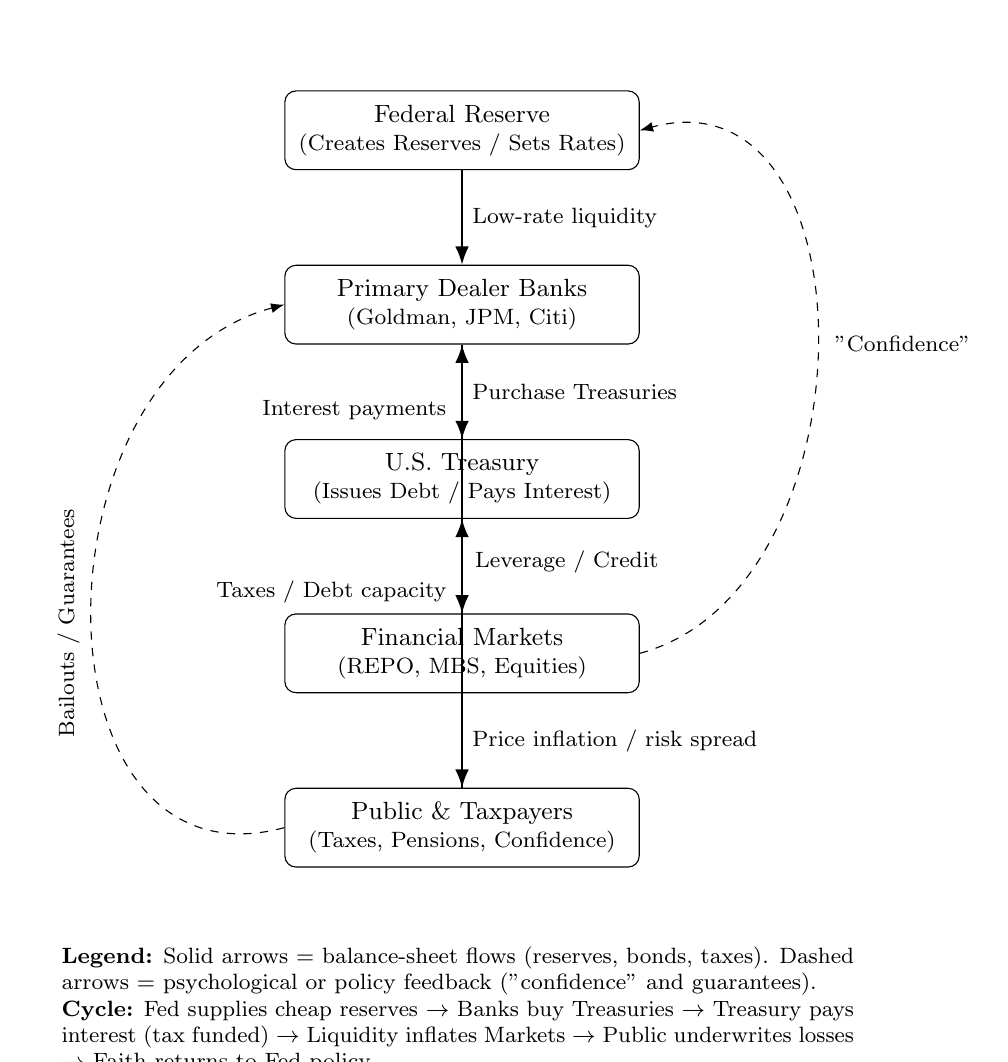
\begin{tikzpicture}[xshift=-2.0cm,  % move whole diagram left
  font=\small,
  node distance=12mm,
  box/.style={draw, rounded corners, align=center,
              minimum width=45mm, minimum height=10mm},
  arrow/.style={-Latex, thick},
  thinarrow/.style={-Latex, dashed}
]

% --- Nodes ---
\node[box] (fed)        {Federal Reserve\\[-1pt]\footnotesize (Creates Reserves / Sets Rates)};
\node[box, below=of fed] (banks)      {Primary Dealer Banks\\[-1pt]\footnotesize (Goldman, JPM, Citi)};
\node[box, below=of banks] (treasury) {U.S. Treasury\\[-1pt]\footnotesize (Issues Debt / Pays Interest)};
\node[box, below=of treasury] (markets) {Financial Markets\\[-1pt]\footnotesize (REPO, MBS, Equities)};
\node[box, below=of markets] (public)  {Public \& Taxpayers\\[-1pt]\footnotesize (Taxes, Pensions, Confidence)};

% --- Core flows (vertical) ---
\draw[arrow] (fed) -- node[right]{\footnotesize Low-rate liquidity} (banks);
\draw[arrow] (banks) -- node[right]{\footnotesize Purchase Treasuries} (treasury);
\draw[arrow] (treasury) -- node[near start, left, xshift=-2pt, yshift=2pt]{\footnotesize Interest payments} (banks);
\draw[arrow] (banks) -- node[midway, right, xshift=1pt, yshift=-30pt]{\footnotesize Leverage / Credit} (markets);
\draw[arrow] (markets) -- node[right]{\footnotesize Price inflation / risk spread} (public);
\draw[arrow] (public)   -- node[near end,  left, xshift=-2pt, yshift=-2pt]{\footnotesize Taxes / Debt capacity} (treasury);

% --- Feedback paths ---
% Dashed "Confidence" loop (right)
\draw[thinarrow]
  (markets.east) to[out=15,in=15,looseness=1.2]
  node[right, xshift=3pt, yshift=0pt]{\footnotesize "Confidence"} (fed.east);

% Dashed "Bailouts" loop (left, label ON curve)
\draw[thinarrow]
  (public.west)
  to[out=195,in=195,looseness=1.3]
  node[midway, sloped, above, xshift=-2pt, yshift=1pt]{\footnotesize Bailouts / Guarantees}
  (banks.west);

% --- Legend block ---
\node[align=left, below=10mm of public, inner sep=0] (legend) {%
\begin{minipage}{0.83\linewidth}\footnotesize
\textbf{Legend:} Solid arrows = balance-sheet flows (reserves, bonds, taxes).  
Dashed arrows = psychological or policy feedback ("confidence" and guarantees).\\
\textbf{Cycle:} Fed supplies cheap reserves $\rightarrow$ Banks buy Treasuries $\rightarrow$  
Treasury pays interest (tax funded) $\rightarrow$ Liquidity inflates Markets $\rightarrow$  
Public underwrites losses $\rightarrow$ Faith returns to Fed policy.
\end{minipage}
};

\end{tikzpicture}
\caption{The Vertical Liquidity Feedback Loop Between the Federal Reserve, Banks, the U.S. Treasury, and the Public.}
\label{fig:vertical-liquidity-loop}
\end{figure}

\vspace{1em}

\begin{tcolorbox}[colback=gray!6!white,colframe=black!25!white,title=\textbf{Appendix: 2008 Crisis Mechanics — Repo, TARP, QE, and Collateral Chains},fonttitle=\bfseries]
\small
\textbf{Repo (Repurchase Agreement) Markets:}  
In 2008, major investment banks like Lehman Brothers and Bear Stearns funded their daily operations by borrowing cash overnight against securities collateral.  
These “repos” were effectively short-term loans disguised as sales.  
When the value of the collateral (mortgage-backed securities) collapsed, counterparties refused to roll over repos.  
Liquidity vanished overnight, freezing the global financial system.

\textbf{Collateral Chains:}  
Banks had rehypothecated the same securities multiple times — using one piece of collateral to back many loans — amplifying leverage across the system.  
When one link failed, the entire chain seized, as each party demanded its own collateral back.  
The illusion of infinite liquidity evaporated.

\textbf{TARP (Troubled Asset Relief Program):}  
To prevent systemic collapse, the U.S. Treasury authorized \$700 billion to recapitalize major banks.  
Institutions like Citigroup, JPMorgan, Goldman Sachs, and Morgan Stanley received direct injections, ostensibly to restore lending but often used to repair their own balance sheets and sustain bonuses.  
Moral hazard became institutionalized: the financial elite learned that failure would be rewarded.

\textbf{Quantitative Easing (QE):}  
The Federal Reserve began purchasing Treasury and mortgage-backed securities on an unprecedented scale, expanding its balance sheet from under \$1 trillion in 2007 to over \$4 trillion by 2014.  
This “printing” of reserves lowered long-term interest rates and inflated asset prices, but did little to revive real investment.  
It institutionalized the loop: the Fed creates money to buy government debt, which finances more debt issuance, which the same banks then trade for profit.

\textbf{The Legacy:}  
What began as emergency intervention became permanent architecture.  
The post-2008 economy operates on endless QE, perpetual repo liquidity, and infinite collateral recycling.  
The system did not heal; it habituated.  
The Great Hollowing thus became self-sustaining — a financial metabolism feeding on its own blood.
\end{tcolorbox}

% \include{chapters/ch40}
\chapter{Reclaiming the Physical World}
\label{ch:40}
% --- TODO: 500--700 word chapter summary in manifesto--narrative tone.
% Use "The Great Hollowing" as the central analytic thread.

Every era defines itself by what it touches.  
The nineteenth century touched steel and steam; the twentieth, electricity and code.  
The twenty-first has touched nothing.  
We live in a civilization that floats above its foundations—its food, its energy, its soil, its hands.  
The factories that once thundered with the noise of labor have fallen silent, replaced by screens that hum with the noise of representation.  
Work has migrated from the field to the feed, from the workshop to the window of a device.  
The human being, once defined by making, is now defined by managing.  
This is the thirty-ninth movement of \textbf{The Great Hollowing}: the disembodiment of existence.
\section*{The Vanishing Substance}

Modern man consumes images of things instead of things themselves.  
He scrolls through pictures of meals while forgetting the taste of bread; he trades digital currencies that promise ownership but never touch matter.  
In the financialized economy, wealth no longer grows from the earth or the forge; it grows from fluctuations in belief.  
The global citizen has become a spectator of his own survival.

The more virtual our life becomes, the more fragile its foundation.  
A world built on abstraction loses its capacity for repair.  
When the network fails, no one remembers how to fix the generator.  
When the supply chain breaks, no one recalls how to plant.  
We have built an empire of convenience that cannot survive inconvenience.  
\textbf{The Great Hollowing} manifests not as scarcity but as disconnection: a famine of contact, a drought of comprehension.

The very language of labor has changed.  
Craftsmanship, once an act of devotion, has been replaced by logistics—by the art of moving goods without touching them.  
Digitalization promised freedom from drudgery, but it delivered alienation from creation.  
A civilization that forgets how to build forgets how to believe.

\section*{The Tyranny of the Virtual}

The dream of frictionless life—instant payment, instant food, instant affirmation—has enslaved us to a realm without resistance.  
The virtual world offers infinite speed but zero texture.  
It flattens space and time, promising omnipresence while erasing presence.  
To exist within it is to live in perpetual elsewhere.  
Our tools, once extensions of our strength, have become replacements for our senses.  
We have traded intimacy for access, depth for data, weight for convenience.

The economist speaks of productivity, the philosopher of progress, but neither can explain why meaning declines as comfort rises.  
The reason is simple: abstraction consumes the real.  
When everything is mediated by code or currency, the hand ceases to know the world.  
The body becomes irrelevant; the face becomes an interface.  
Reality itself becomes negotiable—a subscription, not a covenant.

\section*{The Ecology of Forgetting}

\textbf{The Great Hollowing} is not only economic but ecological.  
A society that views nature as inventory inevitably forgets that it is nature.  
We speak of “resources” as if the earth were a spreadsheet, as if forests were columns of carbon, as if rivers could be optimized.  
We live in buildings that seal us from weather, eat food that arrives without soil, and design policies to manage the planet as if it were a portfolio.

The result is a new metaphysical poverty: the inability to imagine the world without us.  
Humanity has become the center of its own simulation.  
We measure the climate not by what it is but by what it costs.  
The environmental crisis is thus not a failure of technology but of ontology—a crisis of relation between creature and creation.

Reclaiming the physical world means restoring reverence.  
It requires more than sustainability; it requires sacrament.  
The soil must cease to be a commodity and return to being a teacher.  
The river must cease to be an input and return to being a boundary between hubris and humility.  
To rebuild the world, we must first re-inhabit it.

\section*{The Return of the Hand}

The recovery of meaning begins with the recovery of touch.  
A craftsman understands reality differently from a manager.  
To shape wood, stone, or metal is to encounter resistance—the world’s polite reminder that one’s ideas are not omnipotent.  
The hand corrects the fantasy of the mind.  
Every hammer strike teaches proportion; every mistake teaches patience.  
In the workshop, truth is not debated but discovered.

Industrial civilization once understood this.  
The builder, the farmer, the mechanic, the sailor—all worked within limits and learned respect for them.  
Now, our heroes are those who transcend limits through leverage: venture capitalists, influencers, algorithmic traders.  
But leverage is only strength borrowed from something solid.  
When the solid disappears, so does the leverage.  
To restore balance, the age of speculation must give way to the age of substance.

Reclaiming the physical world does not mean rejecting technology; it means re-anchoring it in matter.  
The digital must serve the tangible, not replace it.  
AI should augment craftsmanship, not annihilate it.  
Automation should reduce toil, not obliterate vocation.  
Technology becomes humane only when it recognizes its material dependencies.

\section*{The Moral Weight of Matter}

A society that loses touch with its physical reality also loses its moral gravity.  
Ethics without embodiment becomes mere preference.  
To act rightly requires consequence; consequence requires contact.  
The detachment of decision from impact—the boardroom making policies for unseen laborers, the investor profiting from distant exploitation—creates the illusion of innocence.  
But matter remembers what minds forget.  
Every product, every click, every purchase leaves a trace in the world that cannot be abstracted away.

\textbf{The Great Hollowing} has created an economy of denial.  
We no longer feel the cost of our conveniences.  
Rare earth minerals mined by invisible hands, oceans clogged by disposable luxury, human attention auctioned to algorithms—all remain hidden beneath the sheen of progress.  
The first act of moral restoration is to see again, to touch again, to feel the weight of our comforts.

\section*{Re-grounding Knowledge and Education}

Education, too, has drifted from the real.  
Students learn theories of sustainability without planting a seed, economics without seeing a workshop, philosophy without encountering silence.  
Knowledge has become simulation: information without experience.  
Reclaiming the physical world means reuniting intellect with embodiment.  
The mind must once again touch what it studies.  
A true university would include a forge, a garden, a kitchen, and a studio—places where thought meets resistance.

Only when the educated class rediscovers friction will leadership recover humility.  
Policy cannot arise from abstraction alone; it must grow from direct contact with consequence.  
A statesman who has repaired a wall or plowed a field will govern differently than one who has only written memos.  
The restoration of civic virtue depends on the re-education of the hand.

\section*{The Political Renewal of Reality}

Politics, once grounded in tangible needs—food, shelter, work—has become a theatre of narratives detached from material life.  
Candidates speak of data and diversity while bridges crumble, aquifers drain, and power grids age.  
A nation that cannot maintain its roads cannot maintain its ideals.  
Infrastructure is not a metaphor but a measure of civilization’s honesty.  
The physical neglect of the public realm mirrors the moral neglect of the common good.

Reclaiming the physical world is therefore a political act.  
It means reasserting that citizenship involves stewardship, not merely opinion.  
A republic cannot endure if it is built entirely on symbols.  
Its laws must be embodied in roads, schools, and rivers that actually function.  
Liberty must once again produce something visible—something that can be held, repaired, and passed on.

\section*{The Return of Limits}

To reclaim the physical world is to rediscover limits not as enemies but as guides.  
The denial of limits—whether ecological, economic, or moral—is the root of modern despair.  
A healthy civilization lives within boundaries: of soil fertility, of human attention, of moral coherence.  
When everything becomes scalable, nothing remains sacred.  
The digital empire sells limitlessness as freedom; the physical world reminds us that freedom without form becomes chaos.

The task ahead is not to destroy the digital but to domesticate it—to bring it back under the authority of human proportion.  
To live within limits is not to regress but to endure.  
The cathedral and the ship, the violin and the bridge—all are miracles of constraint.  
It is through resistance that harmony is born.

\section*{The Spiritual Dimension of Matter}

Matter, in its quiet way, is sacred.  
To touch it is to encounter the mystery of existence—the same mystery that once drew artists to marble and saints to fasting.  
When humanity ceases to respect the material, it also ceases to respect the invisible that moves through it.  
The division between the physical and the spiritual is false; both require presence, both demand attention.  
A culture that neglects matter will inevitably trivialize spirit.

Reclaiming the physical world is thus an act of metaphysical rebellion.  
It is the refusal to live entirely inside representation.  
It is the rediscovery that the sacred begins not in symbols but in substance—in bread broken, in water drawn, in labor honestly done.  
To rebuild civilization, we must first remember that the world we inherit is not a screen but a body.

\section*{The End of the Hollowing}

When the digital storm passes—and it will—what will remain are the things that resist replication: the soil, the stone, the human face.  
The economy of the future will not belong to those who manipulate signs but to those who restore meaning.  
The craftsman will again be honored, the teacher of patience, the farmer of renewal, the builder of memory.  
The measure of civilization will not be its connectivity but its contact.

\textbf{The Great Hollowing} began when humanity abandoned matter for models.  
It will end when we return, not nostalgically, but reverently.  
The world does not need to be reinvented—it needs to be remembered.  
To reclaim the physical world is to reclaim reality itself, and with it, the dignity of being human.

% \include{chapters/ch41}
\chapter{After the Hollowing: The Moral Reconstruction of Civilization}
\label{ch:41}
% --- TODO: 500--700 word chapter summary in manifesto--narrative tone.
% Use "The Great Hollowing" as the central analytic thread.

Every age of collapse prepares the ground for renewal.  
When illusions fail, reality returns.  
The Great Hollowing—the long detachment of humanity from work, matter, and meaning—has reached its natural conclusion.  
The world of appearances has exhausted itself.  
The screens that once promised infinity now reflect only fatigue.  
The data that once claimed to explain everything explain nothing about why we live, love, or build.  
Civilization has looked into its own mirror and found it empty.  
What comes next must begin where modernity ended: with the reconstruction of the moral world.

\section*{1. The End of Abstraction}

For three centuries, the West believed that reason alone could replace religion, that markets could replace morality, and that progress could replace purpose.  
It built its towers of glass and code upon that faith.  
But abstraction has limits.  
A society cannot live forever by converting reality into representation—by mistaking growth for goodness and metrics for meaning.  
When the symbols cease to correspond to the real, collapse follows.  
We have reached that threshold.

The end of abstraction does not mean the end of knowledge.  
It means the return of knowledge to proportion—science in service of life rather than domination, economy in service of community rather than speculation.  
The moral reconstruction begins when truth is once again measured by coherence with being, not by convenience to power.

\section*{2. The Moral Law of Limits}

Civilization endures only when it recognizes limits.  
The digital empire promised limitlessness—endless consumption, endless credit, endless growth—and in so doing it destroyed the conditions of continuity.  
Now we rediscover what ancient wisdom always knew: that limit is the mother of form.  
The river does not resent its banks; it depends on them.  
Freedom without boundary becomes destruction.  
Ethics, likewise, arises not from indulgence but from restraint—the self-discipline that allows beauty and order to exist.

To rebuild civilization, we must restore the grammar of limitation: attention rather than acceleration, stewardship rather than exploitation, obligation rather than appetite.  
The new moral law is not new at all—it is the oldest one: harmony between human desire and cosmic proportion.

\section*{3. The Return of the Real}

Reconstruction begins with the tangible.  
A culture that no longer builds must learn again how to shape.  
The future will belong to those who can repair, cultivate, and compose—the masons of the digital ruins.  
Cities must be designed for community, not congestion.  
Work must create value beyond profit.  
Education must cultivate wisdom, not merely credentials.  
Each act that restores the link between hand and mind, matter and meaning, becomes a moral act.

In this renewal, the craftsman becomes philosopher, and the philosopher must once again become a builder.  
The new virtue is not innovation but integration—the art of reconnecting what has been separated.  
In rebuilding the physical world, we rebuild the moral one.

\section*{4. The Economy of Reverence}

The hollowed age measured value by velocity; the coming age will measure it by care.  
The Great Hollowing taught that efficiency without empathy is extraction, and wealth without gratitude is rot.  
The reconstruction demands an economy that honors creation rather than consumption.  
This means re-embedding money in meaning:  
finance that serves production, production that serves community, and community that serves life.  
The economy must cease to be a machine and become a covenant—a reciprocal exchange between effort and sustenance.

Reverence is not sentimentality.  
It is the recognition that the world possesses intrinsic worth beyond utility.  
To treat nature, labor, and knowledge with reverence is to remember that they are not ours to exploit but ours to protect.  
A civilization without reverence becomes clever but cruel.  
A civilization with it becomes wise.

\section*{5. The Political Restoration of Virtue}

The crisis of politics is not corruption; it is confusion.  
Modern democracies mistake procedure for principle.  
They vote, but they no longer deliberate.  
They speak of rights but forget responsibilities.  
The reconstruction of civilization will require a new political philosophy—one that unites freedom with duty.  
The republic must cease to be a marketplace of promises and become again a forum of conscience.

This restoration will not come from ideology but from example.  
Leaders who live with integrity will inspire trust more than those who legislate it.  
Authority must be earned through service, not granted by spectacle.  
In an age of manipulation, honesty itself becomes revolutionary.

The civic oath of the future will be simple: to act in such a way that one’s gain does not hollow the world of another.

\section*{6. The Spiritual Reawakening}

The hollowing was not merely social; it was spiritual.  
It began when the sacred was privatized—confined to preference rather than woven into the pattern of life.  
To reconstruct civilization, the sacred must return, not as dogma but as dimension.  
Every true culture arises from a sense of the infinite mirrored in the finite: the temple, the song, the child, the sunrise.  
To live without that sense is to die slowly in distraction.

The spiritual renewal of the coming age will not be uniform.  
It may appear in Orthodox cathedrals, in Sufi poetry, in Zen gardens, in the quiet conscience of scientists who rediscover wonder.  
Its unity will not be in creed but in humility—the recognition that existence precedes ownership and that creation exceeds calculation.

Where the hollowing emptied life of reverence, the reconstruction must fill it with gratitude.

\section*{7. Education of the Soul}

To rebuild civilization, we must educate differently.  
Our schools have produced specialists without wisdom, citizens without virtue, and workers without craft.  
The moral reconstruction must teach not only how to make a living but how to live.  
Knowledge must again be formative, not merely informative—an apprenticeship of the soul.

History should no longer be taught as a sequence of progress but as a study of proportion—how balance is gained and lost.  
Philosophy should not be optional; it should be the core of citizenship.  
Science must learn humility before complexity.  
Technology must be taught alongside ethics, economics alongside ecology.  
The measure of education will be not the number of graduates but the number of guardians it produces.

\section*{8. The Reconstruction of Community}

Community is the architecture of meaning.  
The hollowing atomized society into solitary consumers; reconstruction must reunite it into neighbors and citizens.  
True community cannot be programmed; it must be cultivated.  
It begins with trust and grows through shared labor.  
A town that builds its own bridge knows itself differently than one that buys it.  
Every local act of cooperation defies the empire of abstraction.

The new civilization will therefore be decentralized yet bound by moral coherence—local economies, local crafts, local governance connected through principles rather than algorithms.  
The global must serve the grounded.  
Only a world of rooted communities can resist the return of managerial totality.

\section*{9. The Role of the Artist and the Poet}

When a civilization forgets its purpose, it is the artist who remembers.  
The artist is not entertainer but midwife of meaning.  
In the reconstruction, art must recover its moral vocation: to reveal truth, not merely provoke sensation.  
The poet will again become a witness of conscience; the musician a keeper of proportion; the architect a servant of beauty.  
A society that pays its bankers more than its builders is not wealthy but unwell.  
Art that restores reverence will heal what economics cannot.

\section*{10. The Civilization to Come}

After the hollowing, civilization must no longer be defined by dominance but by depth.  
Its greatness will not be measured by skyscrapers or GDP but by the integrity of its smallest acts.  
The world must move from the age of acceleration to the age of attention.  
The question will not be how much we can produce, but how much meaning we can preserve.

In this new epoch, technology will remain, but it will serve life instead of simulating it.  
Finance will persist, but it will fund creation rather than consumption.  
Governments will exist, but they will protect form rather than dictate thought.  
The new civilization will not abolish modernity—it will complete it by reuniting it with morality.

\section*{11. The Final Lesson of The Great Hollowing}

\textbf{The Great Hollowing} has revealed the ultimate truth of the human condition: that progress without purpose devours itself.  
The more perfectly the system functions, the less meaning it provides.  
When everything becomes easy, nothing remains essential.  
The cure is not nostalgia but remembrance.  
We must remember what our ancestors knew without machines: that life is not an algorithm, that the sacred is not optional, and that civilization survives only when it knows what it stands for.

The moral reconstruction of civilization will not be decreed; it will be lived—patiently, locally, reverently.  
It begins every time a person chooses integrity over advantage, beauty over noise, craftsmanship over convenience, truth over comfort.  
From such acts, a new world quietly forms.

\section*{12. The Covenant Restored}

Civilization is not a machine; it is a covenant between the living, the dead, and the unborn.  
We are its stewards, not its owners.  
To rebuild it is to honor that trust.  
If the hollowing has taught us anything, it is that we cannot escape the consequences of our abstractions.  
The world we hollowed is the world we must now heal.

The reconstruction will not begin with declarations but with silence—with the pause before creation, the breath before the word.  
In that silence, conscience speaks again.  
And from it arises a civilization that remembers its soul.

\textbf{The Great Hollowing} ends not in despair but in clarity.  
The age of illusion is over.  
The age of meaning begins.

% \include{chapters/ch42}

\chapter{Conclusion: The End of Illusion}
\label{ch:42}
% --- 1000-word conclusion written in manifesto–narrative tone.
% Central thread: "The Great Hollowing" reaches its final stage — revelation and reckoning.

Every empire ends not when it falls, but when it can no longer tell the truth about itself.  
The Great Hollowing began as a quiet shift in language — a replacement of doing with saying, of substance with symbol, of production with presentation.  It grew into a civilization-wide hypnosis, where balance sheets replaced ethics, and image replaced integrity.  What began as management became mythology.  The corporation learned to imitate creation, governments learned to imitate justice, and citizens learned to imitate belief.  Now, at the edge of exhaustion, the illusion no longer holds.

For more than a century, Western capitalism survived by converting everything solid into story.  Labor became “human resources.”  Debt became “growth.”  Extraction became “innovation.”  Each word was a spell cast to disguise decline as progress.  But spells fade when repetition outruns meaning.  The new century reveals the exhaustion of the narrative machine: productivity flat, wages stagnant, institutions hollow, and faith evaporating.  Even the algorithms that were meant to automate belief now consume it faster than it can be produced.

The Great Hollowing was never simply economic; it was spiritual.  A system that once promised liberation through material abundance now produces scarcity of purpose.  Its citizens are wealthier yet more anxious, connected yet more alone, informed yet more disoriented.  The digital empire offers infinite information but no wisdom.  The marketplace promises empowerment while monetizing despair.  A world that once worshiped God now worships “engagement metrics,” and the only remaining transcendence is the illusion of visibility.

Illusions, however, depend on energy — the continuous maintenance of spectacle.  When that energy fades, when the audience looks away, truth re-enters the room.  And truth, once seen, cannot be unseen.  The end of illusion is not catastrophe; it is revelation.  It is the moment when citizens realize that their economic servitude is not destiny but design — that the prosperity of a few was engineered from the exhaustion of the many.  The system was not broken; it was built this way.

At this point, the old rituals have lost their power.  The IPO, the quarterly earnings call, the televised debate, the “breaking news” alert — all perform their cycles without conviction.  Their language still flows, but the faith that sustained it is gone.  The Great Hollowing has reached its natural limit: there is nothing left to hollow out.  Management has consumed the worker, finance has consumed industry, image has consumed meaning, and the machine now feeds upon itself.

And yet, within collapse lies clarity.  When illusion ends, attention returns to what is real: the hands that build, the minds that learn, the earth that endures.  The reconstruction of civilization will not come from policy, but from rediscovery — of craft, of community, of truth earned rather than sold.  The next economy will belong to those who restore coherence between word and deed, symbol and substance.  It will begin not on trading floors but in workshops, laboratories, and neighborhoods where production still retains its moral dimension.

The illusion of freedom through markets must give way to freedom through meaning.  The illusion of wealth through speculation must yield to wealth through contribution.  The illusion of democracy through consumption must be replaced by democracy through participation.  To reclaim reality is not nostalgia; it is survival.  Without reality, even power cannot persist — it becomes a mirage chasing its own reflection.

The task ahead is neither utopian nor sentimental.  It is architectural.  We must rebuild institutions that align truth with function, production with purpose, and governance with accountability.  Economics must again answer to ethics; technology must answer to humanity.  The future will not be found in cloud servers or central banks, but in the re-rooting of value to material, measurable, and moral foundations.  The new frontier is not digital; it is real.

As \textbf{The Great Hollowing} draws to a close, the question remains: what comes after illusion?  The answer is simple but difficult — responsibility.  The freedom to consume without consequence, to speculate without service, to speak without truth, must end.  Civilization cannot survive as an economy of excuses.  The next age will demand something rarer than innovation: integrity.

History suggests that great eras do not end in fire, but in fatigue.  When the performance ceases to convince, when the actors forget their lines, the audience quietly leaves.  So too with us.  The curtain falls not with a crash but with a sigh — and beyond the silence, the sound of real work begins again.

Perhaps that is redemption enough.  To rebuild what was lost, to mean what we say, to make what we need.  To measure progress not in growth, but in coherence.  That is the end of illusion — and the beginning of civilization again.

\chapter*{Afterword: The Post-Industrial Republic}
\addcontentsline{toc}{chapter}{Afterword: The Post-Industrial Republic}

\epigraph{
“Those who build the future must first reclaim the materials of meaning.”\\
— A.V.
}{}

History does not end in collapse; it resets its foundations.  
The Great Hollowing has stripped modern civilization to its frame — exposing the scaffolding of finance, propaganda, and managed belief that once passed for structure.  What remains is not ruin but blueprint.  Beneath the exhaustion of our institutions lies the raw material for something older and newer at once: a republic not of consumers, but of creators.

\textbf{The Post-Industrial Republic} begins where illusion ends.  It asks what comes after the spectacle — when value must again be built, not branded; when citizenship must mean contribution, not commentary.  It imagines an economy of locality, durability, and moral clarity — one in which production is re-embedded in community, and technology serves coherence instead of distraction.  In this new order, work becomes a form of citizenship, and creation a form of resistance.

The future will not be designed in boardrooms or predicted by algorithms.  It will emerge in workshops, cooperatives, laboratories, and networks of trust — among those who remember that civilization was always a manual art.  A society that rebuilds itself must first re-educate its senses: to see again what is real, to measure again what is just, to value again what endures.

The Great Hollowing taught us what happens when symbols devour substance.  
The next era must reverse the equation.  The republic to come will not abolish the market, but re-ensoul it; not destroy technology, but domesticate it; not retreat from progress, but restore proportion to it.  It will be guided not by quarterly metrics but by perennial questions: What is worth making? What is worth keeping? What is worth believing?

Every age inherits the illusions it is strong enough to destroy.  Ours has finally grown strong enough to outgrow its own mythology.  What comes next will not be perfect, but it can be honest — and that, after so long a masquerade, will feel revolutionary.

\vspace{2em}
\begin{flushright}
\textit{Antonios Valamontes}\\
Tampa–Florida, 2025
\end{flushright}

%\backmatter
%\include{backmatter/appendices}
%\include{backmatter/bibliography}

\chapter*{Bibliography}
\addcontentsline{toc}{chapter}{Bibliography}

\begin{thebibliography}{99}

\bibitem{Chandler1977}
Chandler, A. D. (1977). \textit{The Visible Hand: The Managerial Revolution in American Business.} Cambridge, MA: Harvard University Press.

\bibitem{Graeber2018}
Graeber, D. (2018). \textit{Bullshit Jobs: A Theory.} New York: Simon \& Schuster.

\bibitem{Mirowski2013}
Mirowski, P. (2013). \textit{Never Let a Serious Crisis Go to Waste: How Neoliberalism Survived the Financial Meltdown.} London: Verso.

\bibitem{Piketty2014}
Piketty, T. (2014). \textit{Capital in the Twenty-First Century.} Cambridge, MA: Harvard University Press.

\bibitem{Zuboff2019}
Zuboff, S. (2019). \textit{The Age of Surveillance Capitalism.} New York: PublicAffairs.

\bibitem{Standing2011}
Standing, G. (2011). \textit{The Precariat: The New Dangerous Class.} London: Bloomsbury Academic.

\bibitem{Harvey2005}
Harvey, D. (2005). \textit{A Brief History of Neoliberalism.} Oxford: Oxford University Press.

\bibitem{Hedges2009}
Hedges, C. (2009). \textit{Empire of Illusion: The End of Literacy and the Triumph of Spectacle.} New York: Nation Books.

\bibitem{Gorton2010}
Gorton, G. (2010). \textit{Slapped by the Invisible Hand: The Panic of 2007.} Oxford: Oxford University Press.

\bibitem{Keynes1936}
Keynes, J. M. (1936). \textit{The General Theory of Employment, Interest, and Money.} London: Macmillan.

\bibitem{Polanyi1944}
Polanyi, K. (1944). \textit{The Great Transformation: The Political and Economic Origins of Our Time.} New York: Rinehart.

\bibitem{Arendt1958}
Arendt, H. (1958). \textit{The Human Condition.} Chicago: University of Chicago Press.

\end{thebibliography}

%\include{backmatter/index}

\end{document}
